\documentclass[compress]{beamer}
\usepackage{ifthen,verbatim}

\newcommand{\isnote}{}
\xdefinecolor{lightyellow}{rgb}{1.,1.,0.25}
\xdefinecolor{darkblue}{rgb}{0.1,0.1,0.7}

%% Uncomment this to get annotations
%% \def\notes{\addtocounter{page}{-1}
%%            \renewcommand{\isnote}{*}
%% 	   \beamertemplateshadingbackground{lightyellow}{white}
%%            \begin{frame}
%%            \frametitle{Notes for the previous page (page \insertpagenumber)}
%%            \itemize}
%% \def\endnotes{\enditemize
%% 	      \end{frame}
%%               \beamertemplateshadingbackground{white}{white}
%%               \renewcommand{\isnote}{}}

%% Uncomment this to not get annotations
\def\notes{\comment}
\def\endnotes{\endcomment}

\setbeamertemplate{navigation symbols}{}
\setbeamertemplate{headline}{\mbox{ } \hfill
\begin{minipage}{5.5 cm}
\vspace{-0.75 cm} \small
\end{minipage} \hfill
\begin{minipage}{4.5 cm}
\vspace{-0.75 cm} \small
\begin{flushright}
\ifthenelse{\equal{\insertpagenumber}{1}}{}{Jim Pivarski \hspace{0.2 cm} \insertpagenumber\isnote/\pageref{numpages}}
\end{flushright}
\end{minipage}\mbox{\hspace{0.2 cm}}\includegraphics[height=1 cm]{../cmslogo} \hspace{0.1 cm} \includegraphics[height=1 cm]{../tamulogo} \hspace{0.01 cm} \vspace{-1.05 cm}}

\newcommand{\s}[1]{{\mbox{\scriptsize #1}}}

\begin{document}
%% \begin{notes}
%% \item This is the annotated version of my talk.
%% \item If you want the version that I am presenting, download the one
%% labeled ``slides'' on Indico (or just ignore these yellow pages).
%% \item The annotated version is provided for extra detail and a written
%% record of comments that I intend to make orally.
%% \item Yellow notes refer to the content on the {\it previous} page.
%% \item All other slides are identical for the two versions.
%% \end{notes}

\small

%% \begin{frame}
%% \frametitle{Outline}
%% \begin{itemize}\setlength{\itemsep}{0.75 cm}
%% \item 
%% \end{itemize}
%% %% \hspace{-0.83 cm} \textcolor{darkblue}{\Large Outline2}
%% \end{frame}

\begin{frame}
\frametitle{Dimuon + orphaned muon}
\begin{itemize}
\item Selection: exactly one dimuon (mu-jet containing two muons) and one ``orphan'' (clean muon not belonging to any mu-jets) with $p_T > 12$~GeV$/c$, $|\eta| < 1$
\item Purpose: the orphan satisfies the trigger, and we get an unbiased view of the dimuon spectrum without having to satisfy the trigger.  This is important for the dimuon-dimuon signal channel, where only one of the two dimuons must satisfy the trigger; the other is generic
\end{itemize}

\begin{columns}
\column{0.5\linewidth}
\centering mass $<$ 3~GeV/$c^2$

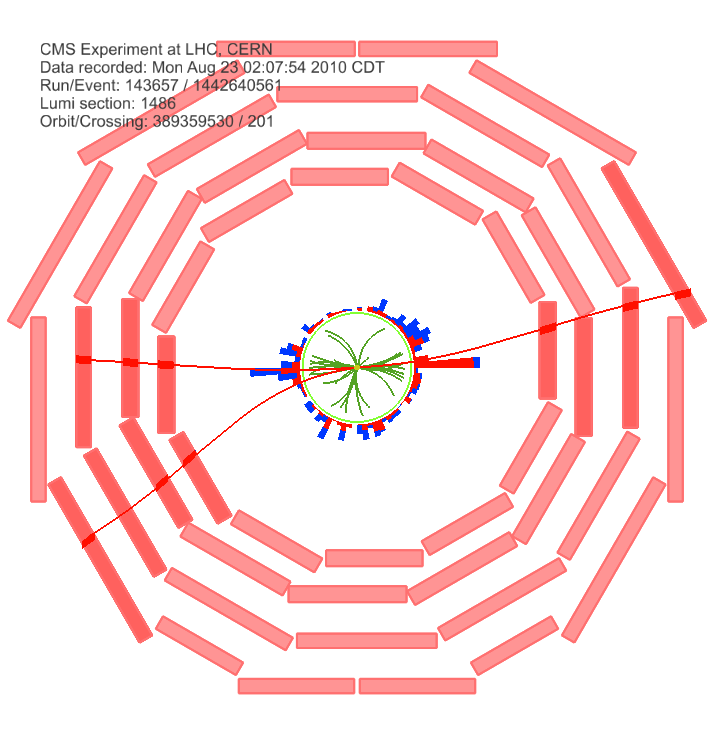
\includegraphics[width=0.8\linewidth]{dimuorphan_eventdisplay_balanced.png}

\column{0.5\linewidth}
\centering mass in $J/\psi$ window

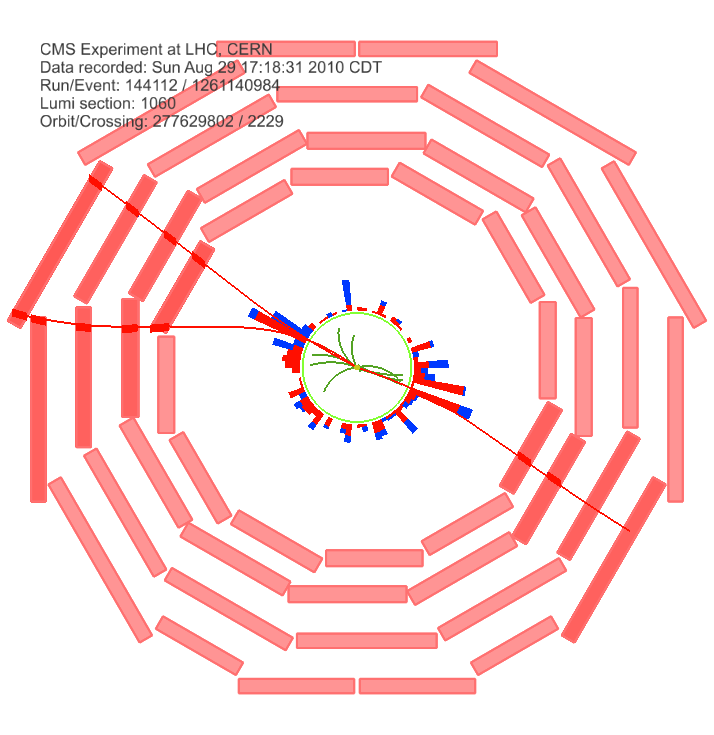
\includegraphics[width=0.8\linewidth]{dimuorphan_eventdisplay_jpsi.png}
\end{columns}
\end{frame}

\begin{frame}
\frametitle{Dimuon spectrum w/o trigger bias}

\begin{itemize}

\item Parameterized background shape:

{\tt \tiny 41.22*exp(-(x-3.096916)**2 / 2. / 0.025**2) + 0.10 + -0.51*(x-5) + -0.97*(x-5)**2 + -0.76*(x-5)**3 + -0.12*(x-5)**4}

\begin{center}
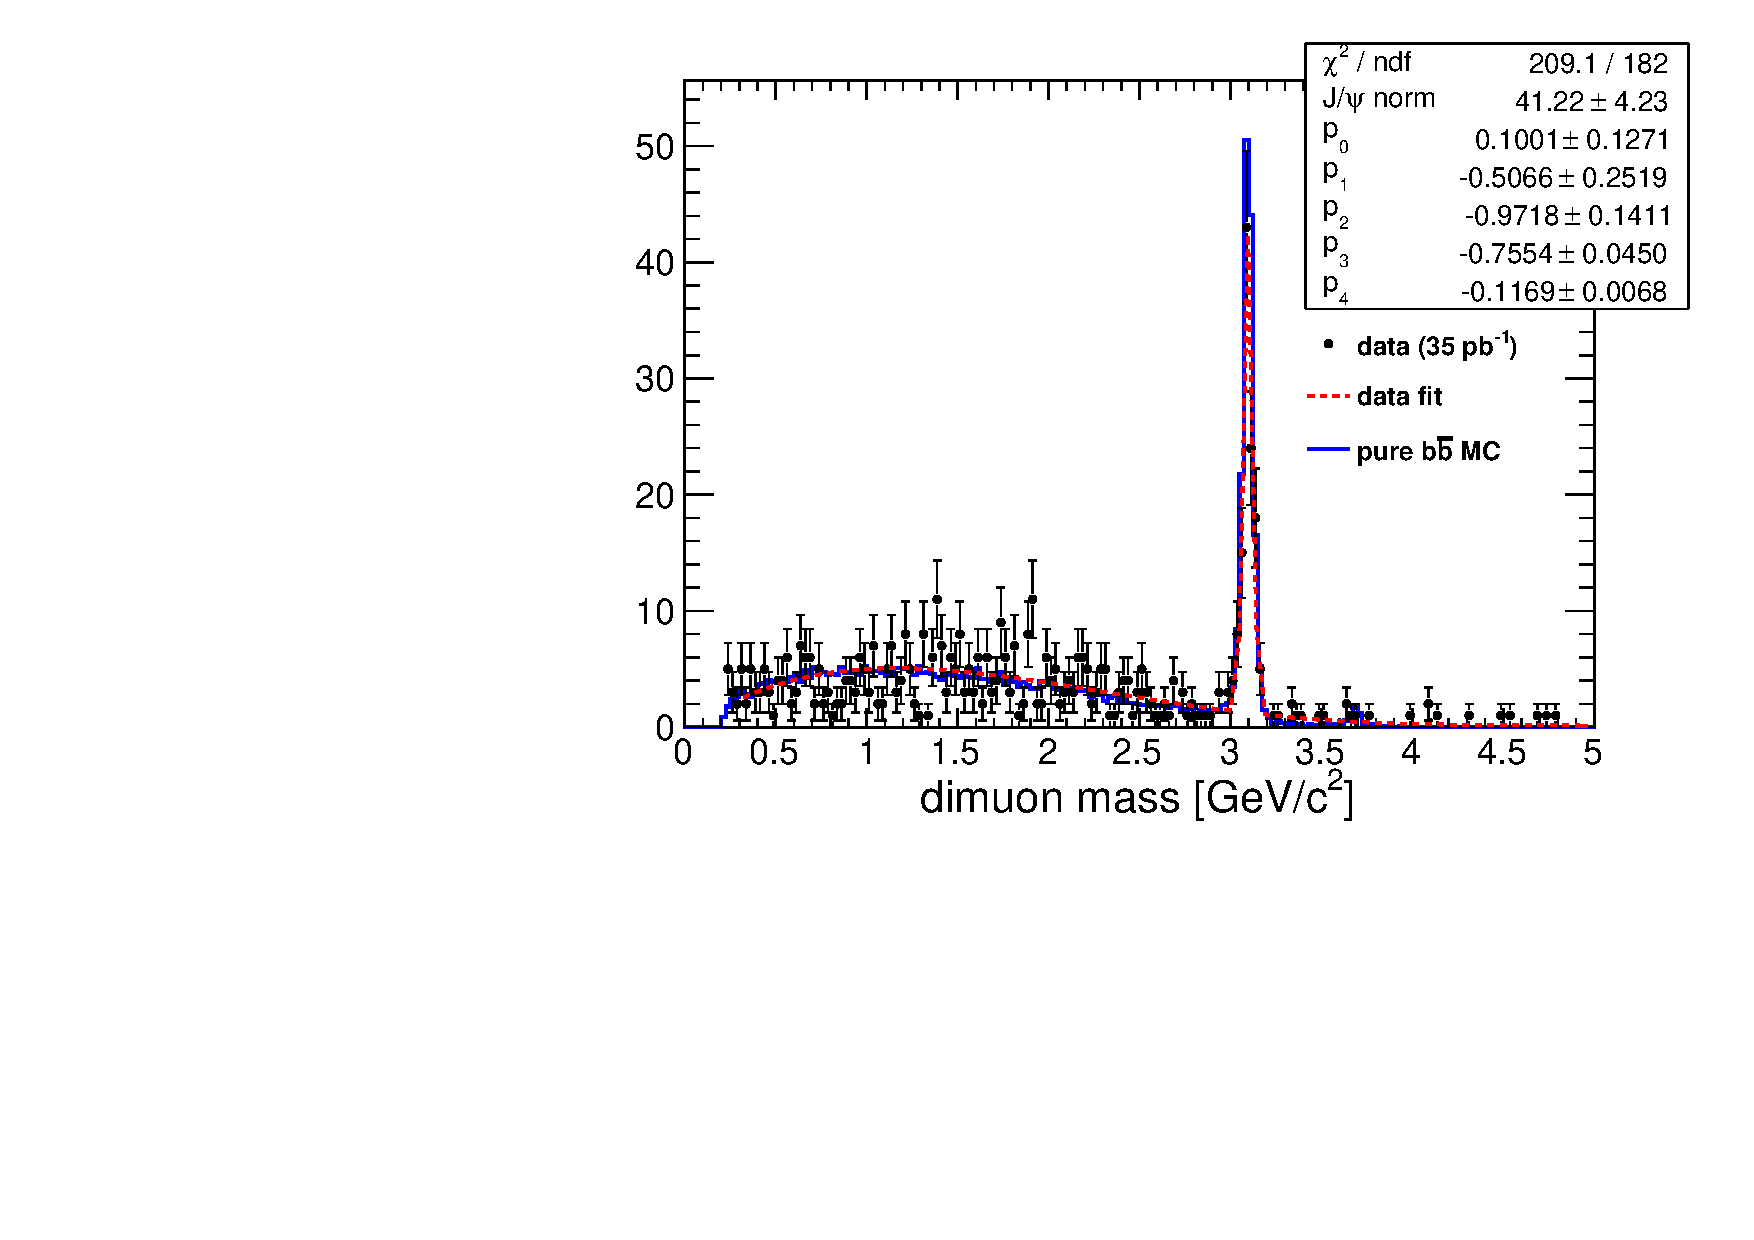
\includegraphics[width=0.6\linewidth]{dimuorphan_mass_fit.pdf}
\end{center}

\item Not enough statistics to see any resonances other than $J/\psi$, but they could be there\ldots perhaps their normalizations need to be nuisance parameters?  {\scriptsize (We ought to have poor sensitivity to new resonances whose mass is exactly equal to a Standard Model resonance, especially when we don't know how many events with that Standard Model resonance to expect.)}
\end{itemize}
\end{frame}

\begin{frame}
\frametitle{Data/MC comparisons}

\begin{itemize}
\item A (very large int.\ lumi.) pure $b\bar{b}$ sample describes the
  observed mass distribution well, but there are discrepancies in some
  of the other variables

\item Azimuthal angle between the dimuon axis and the orphan muon:

\begin{center}
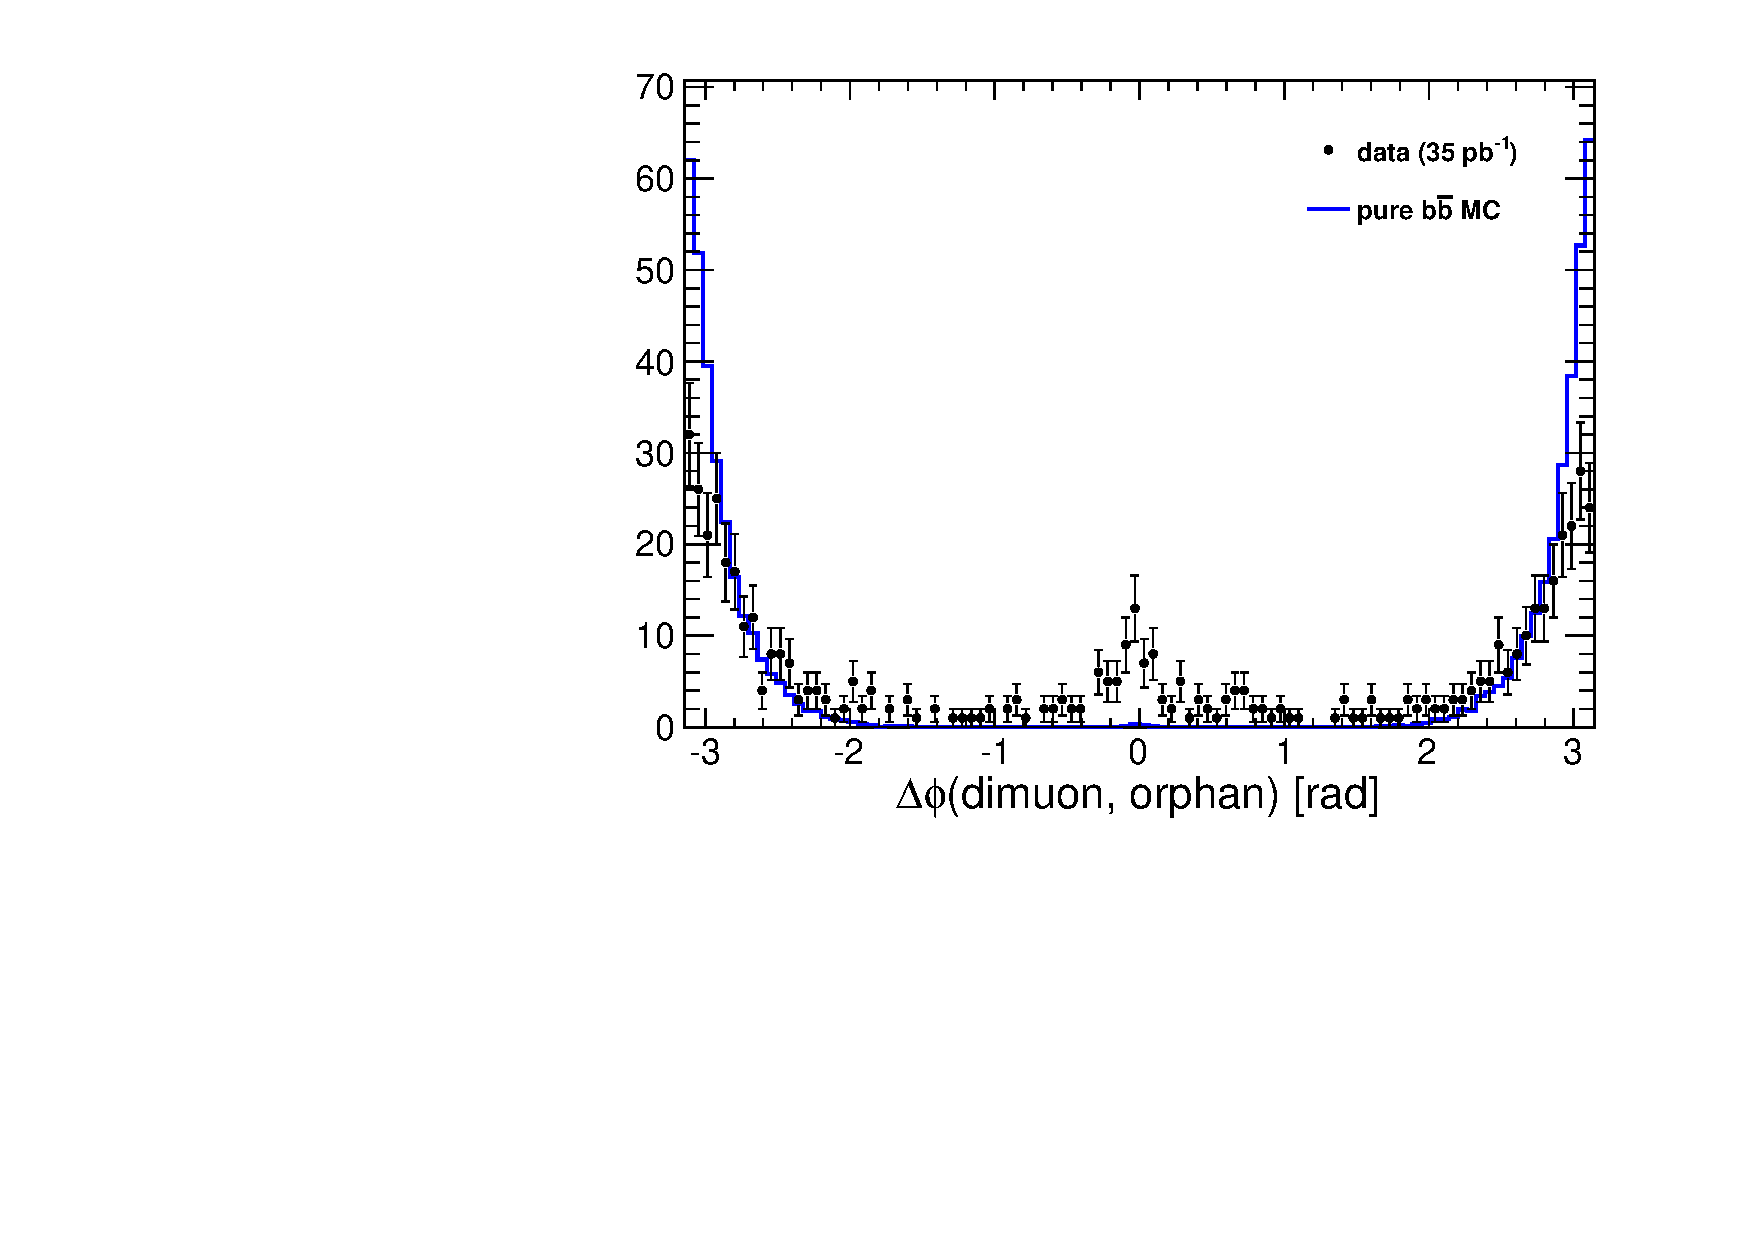
\includegraphics[width=0.7\linewidth]{dimuorphan_deltaphi.pdf}
\end{center}

\item MC is almost perfectly back-to-back, but data isn't
\end{itemize}
\end{frame}

\begin{frame}
\frametitle{Examples of acolinearity in data}
\begin{columns}
\column{0.5\linewidth}
\centering Example in data of a third jet unbalancing the $b\bar{b}$ {\scriptsize (with punch-through!)}

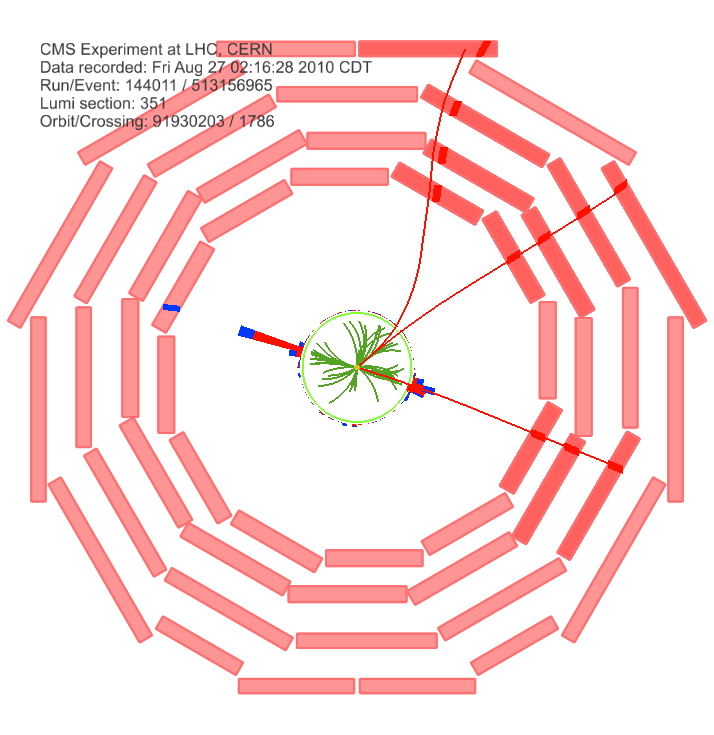
\includegraphics[width=\linewidth]{dimuorphan_eventdisplay_thirdjet.png}

\column{0.5\linewidth}
\centering Example in data of dimuon offset from the center of its jet

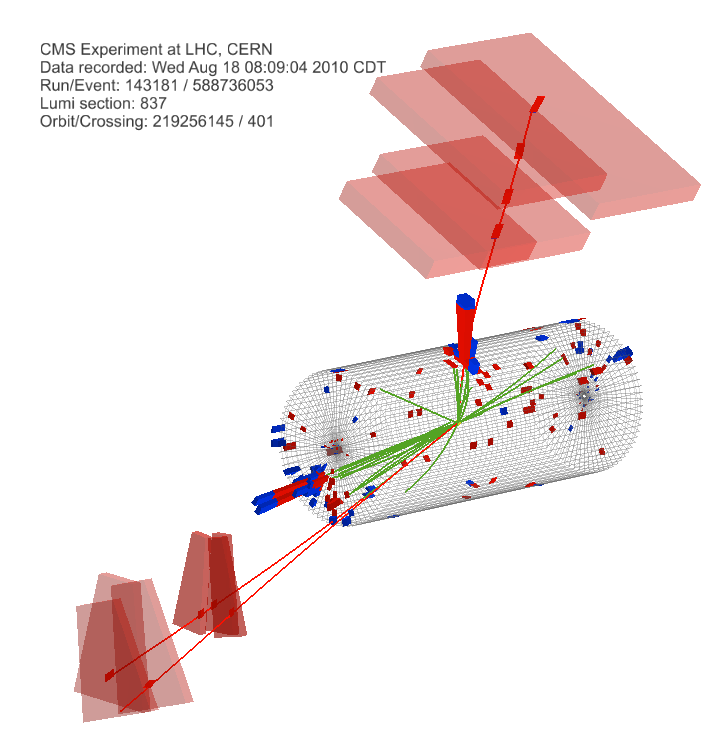
\includegraphics[width=\linewidth]{dimuorphan_eventdisplay_outofjet.png}
\end{columns}

These effects boost the $b$-quark systems, but invariant mass (our
quantity of interest) is insensitive to external boosts
\end{frame}

\begin{frame}
\frametitle{More data/MC comparisons}

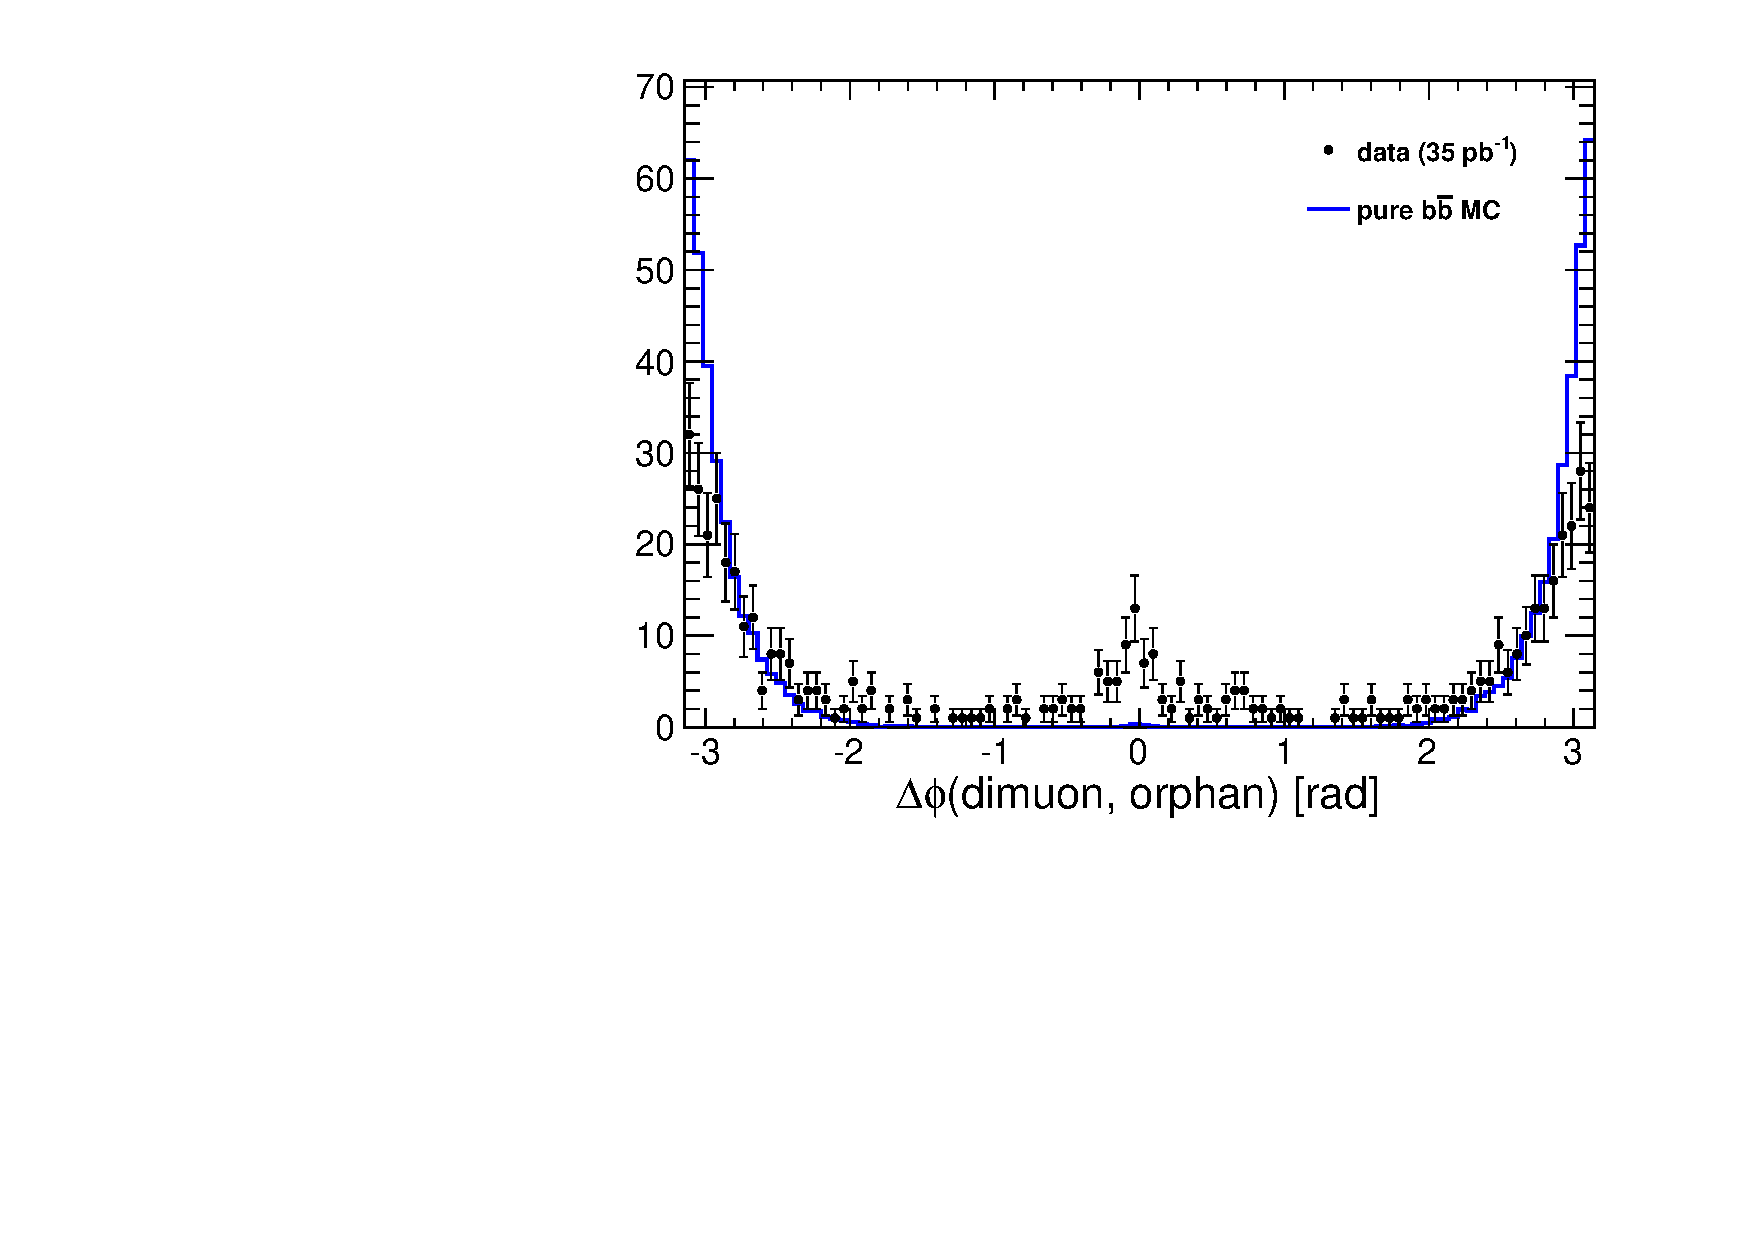
\includegraphics[width=0.5\linewidth]{dimuorphan_deltaphi.pdf}
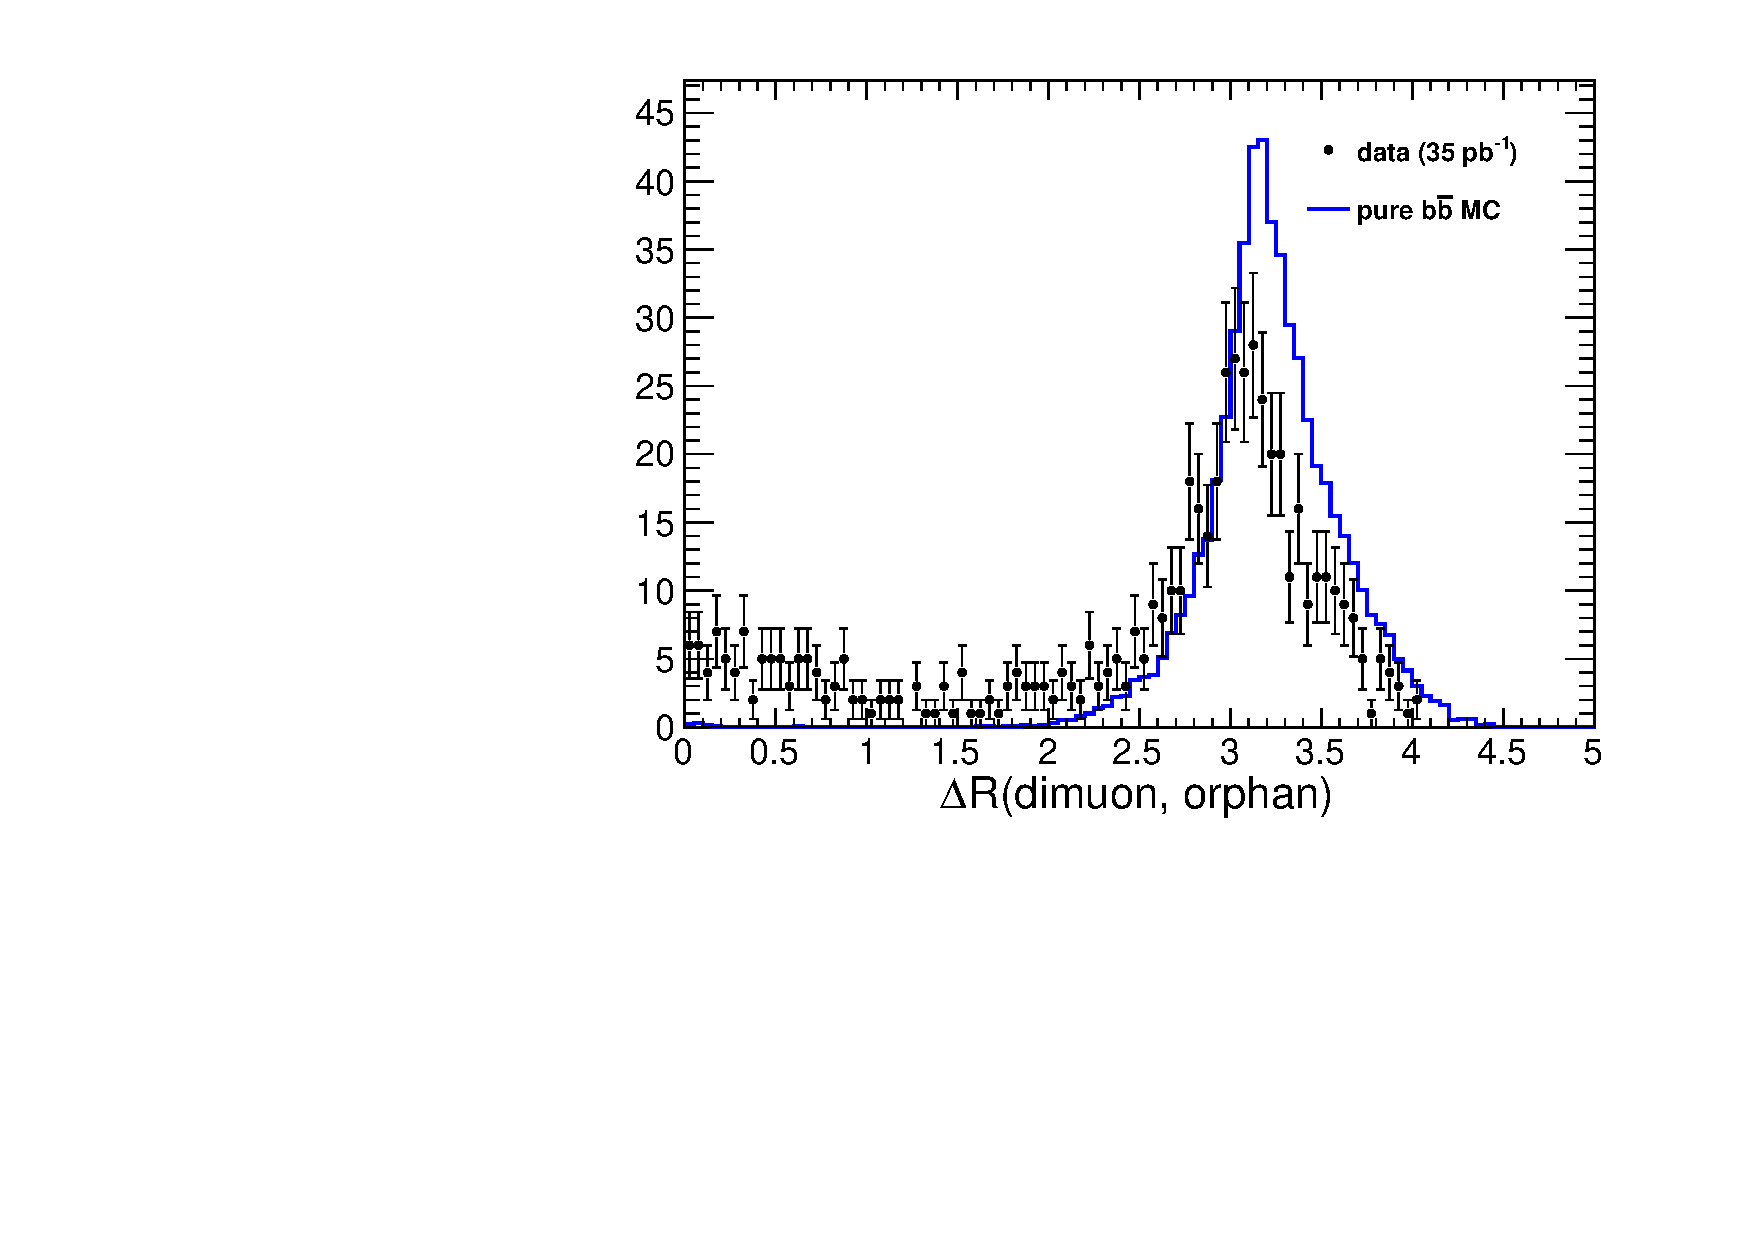
\includegraphics[width=0.5\linewidth]{dimuorphan_deltar.pdf}

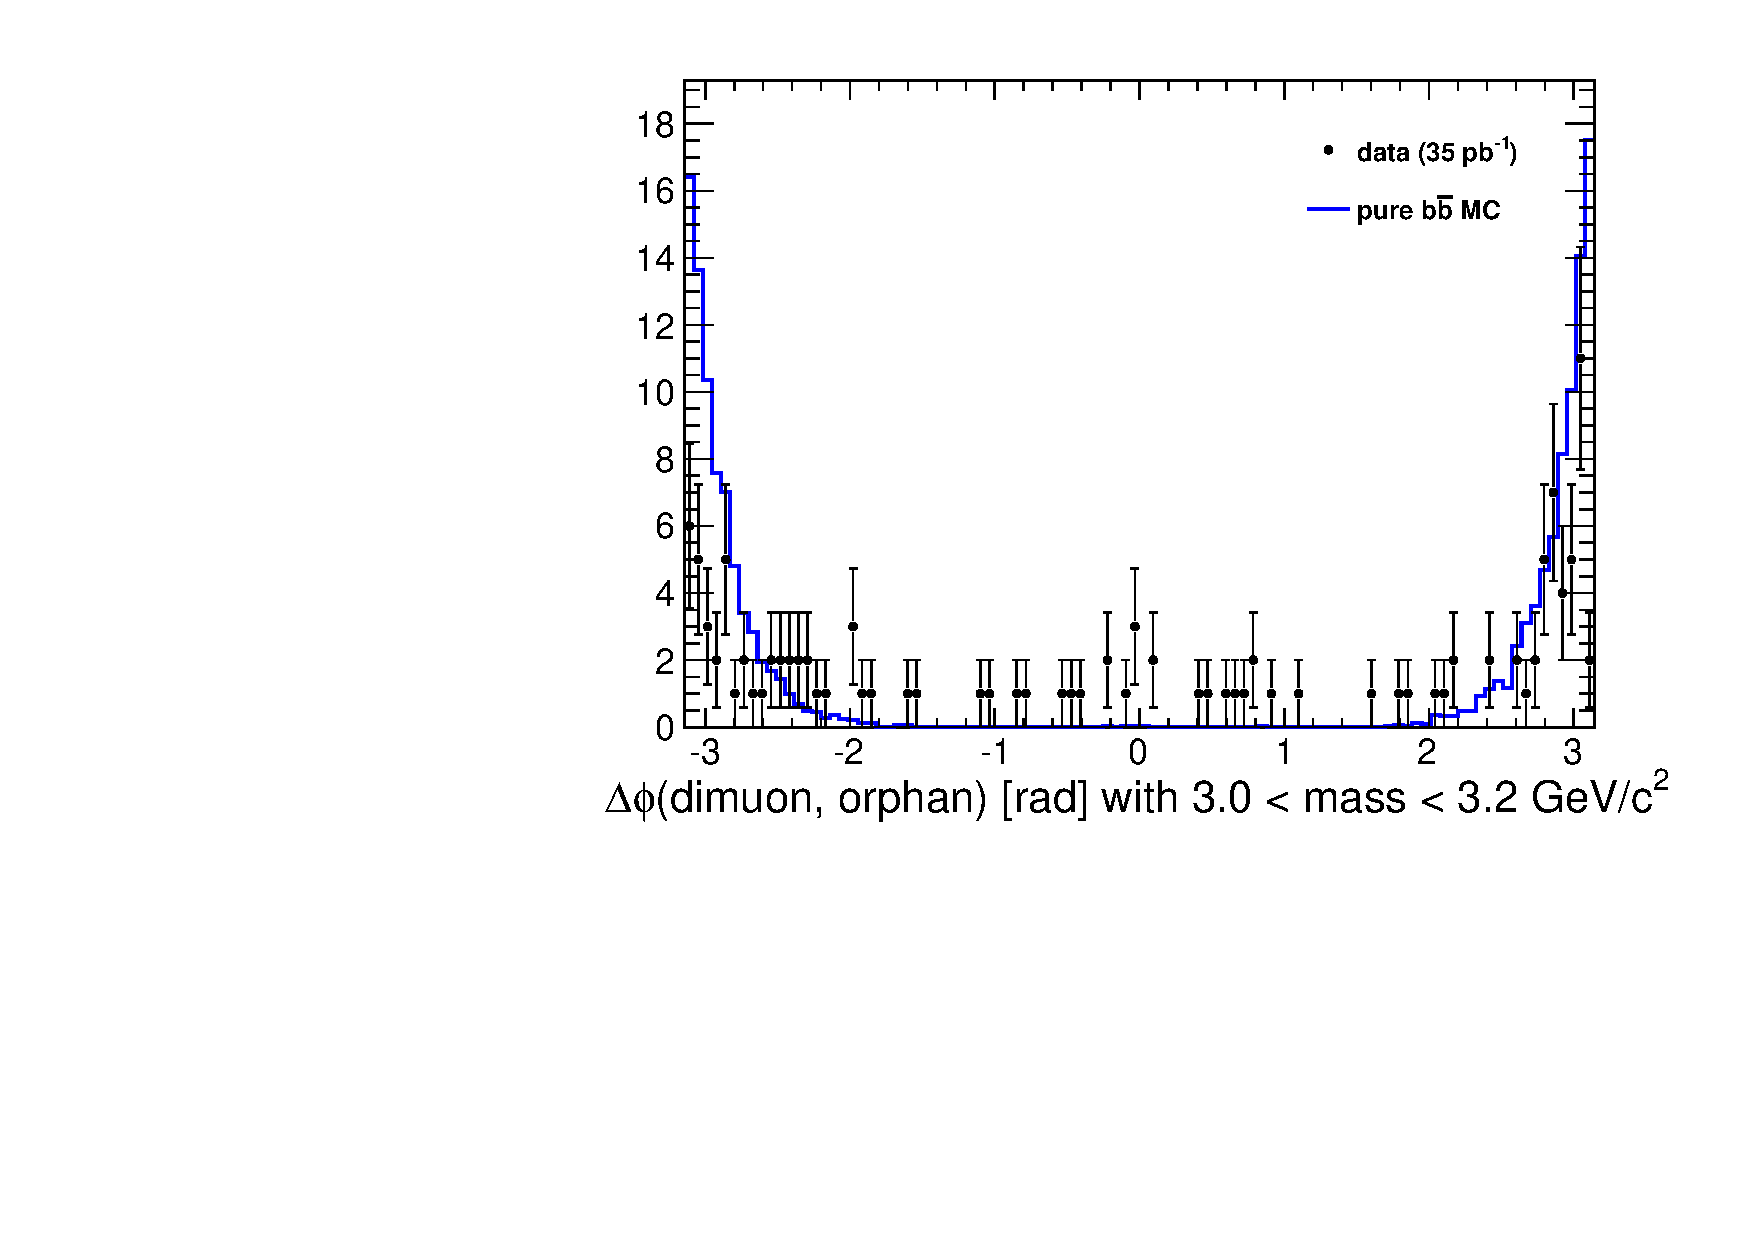
\includegraphics[width=0.5\linewidth]{dimuorphan_deltaphi_jpsi.pdf}
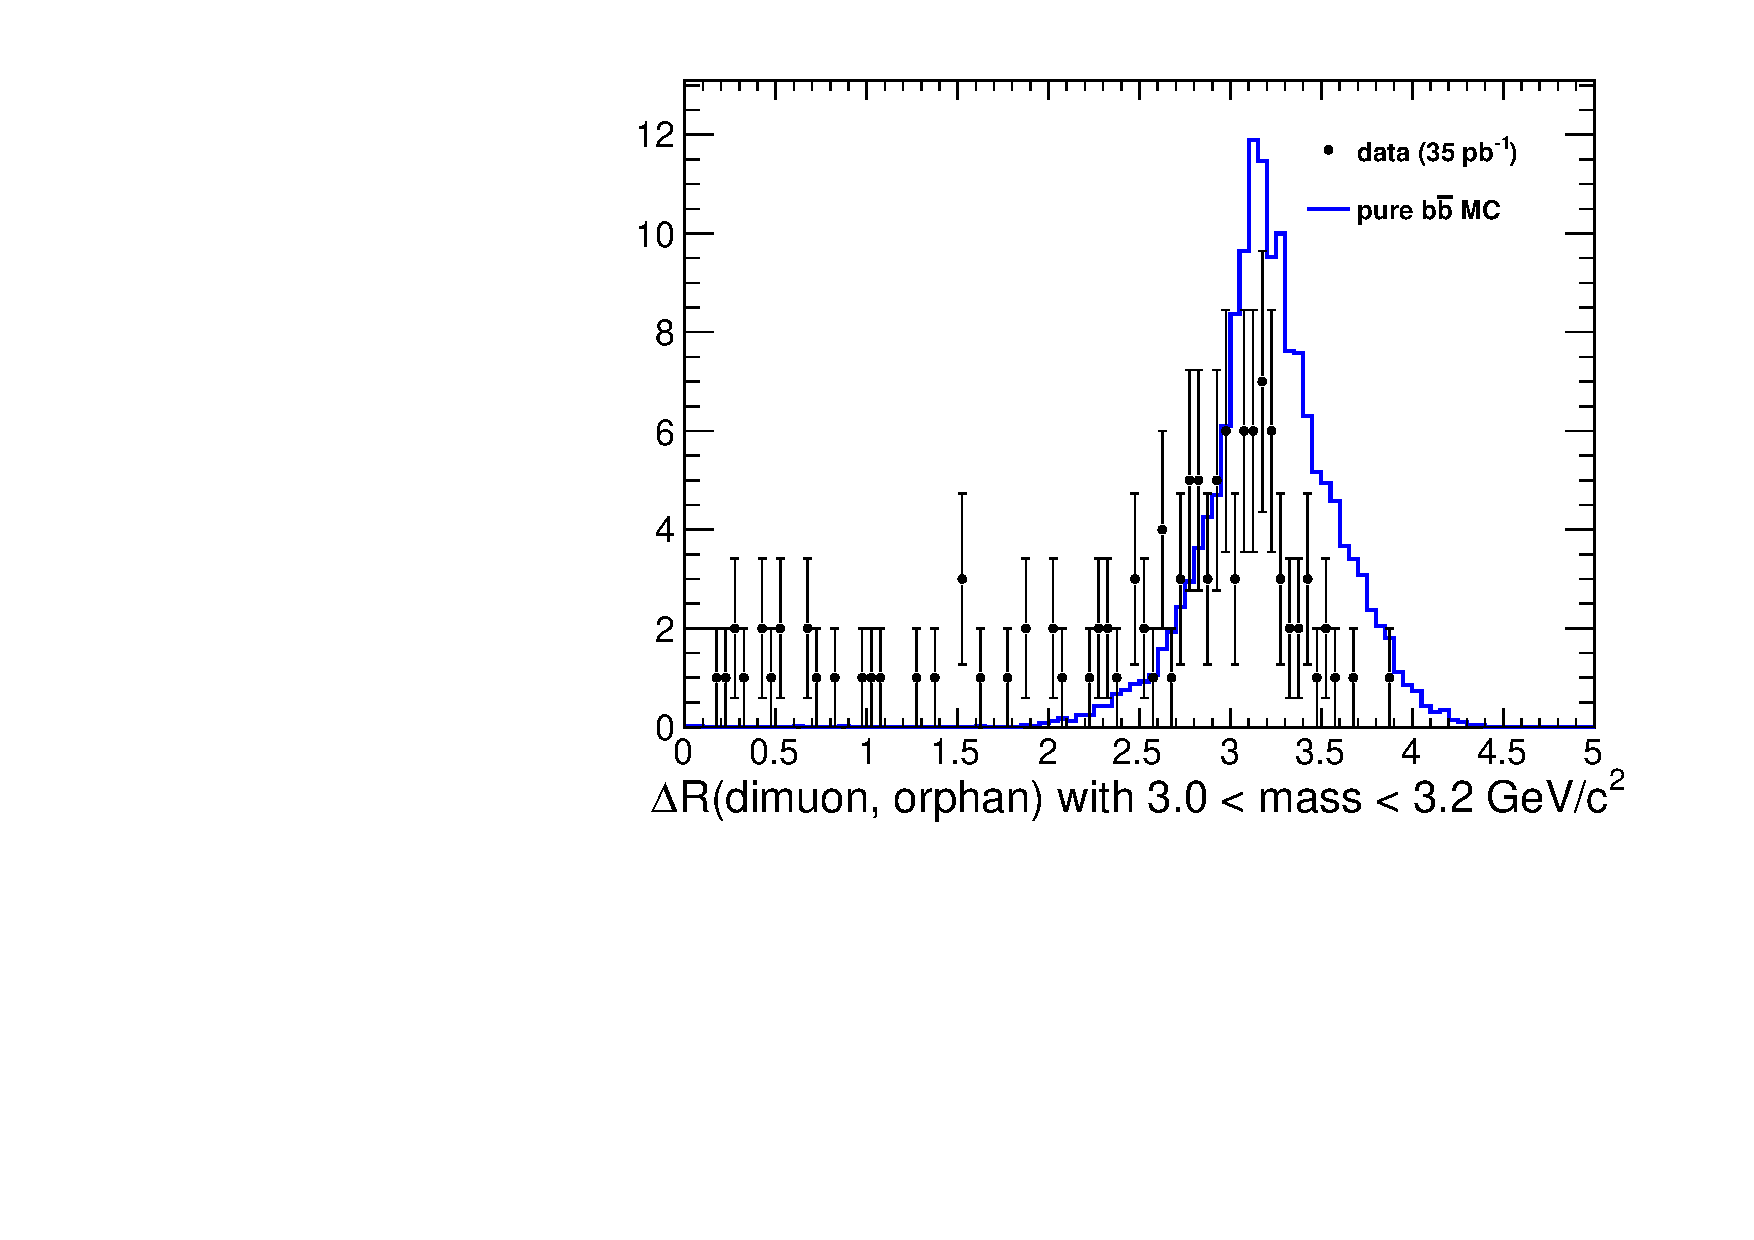
\includegraphics[width=0.5\linewidth]{dimuorphan_deltar_jpsi.pdf}
\end{frame}

\begin{frame}
\frametitle{More data/MC comparisons}

\begin{itemize}
\item $p_T$ and $\eta$ of the dimuon, the orphan, and both
\item Only problem is the vector-sum $p_T$ of both, since the whole
  system is boosted differently in data than it is in MC
\end{itemize}

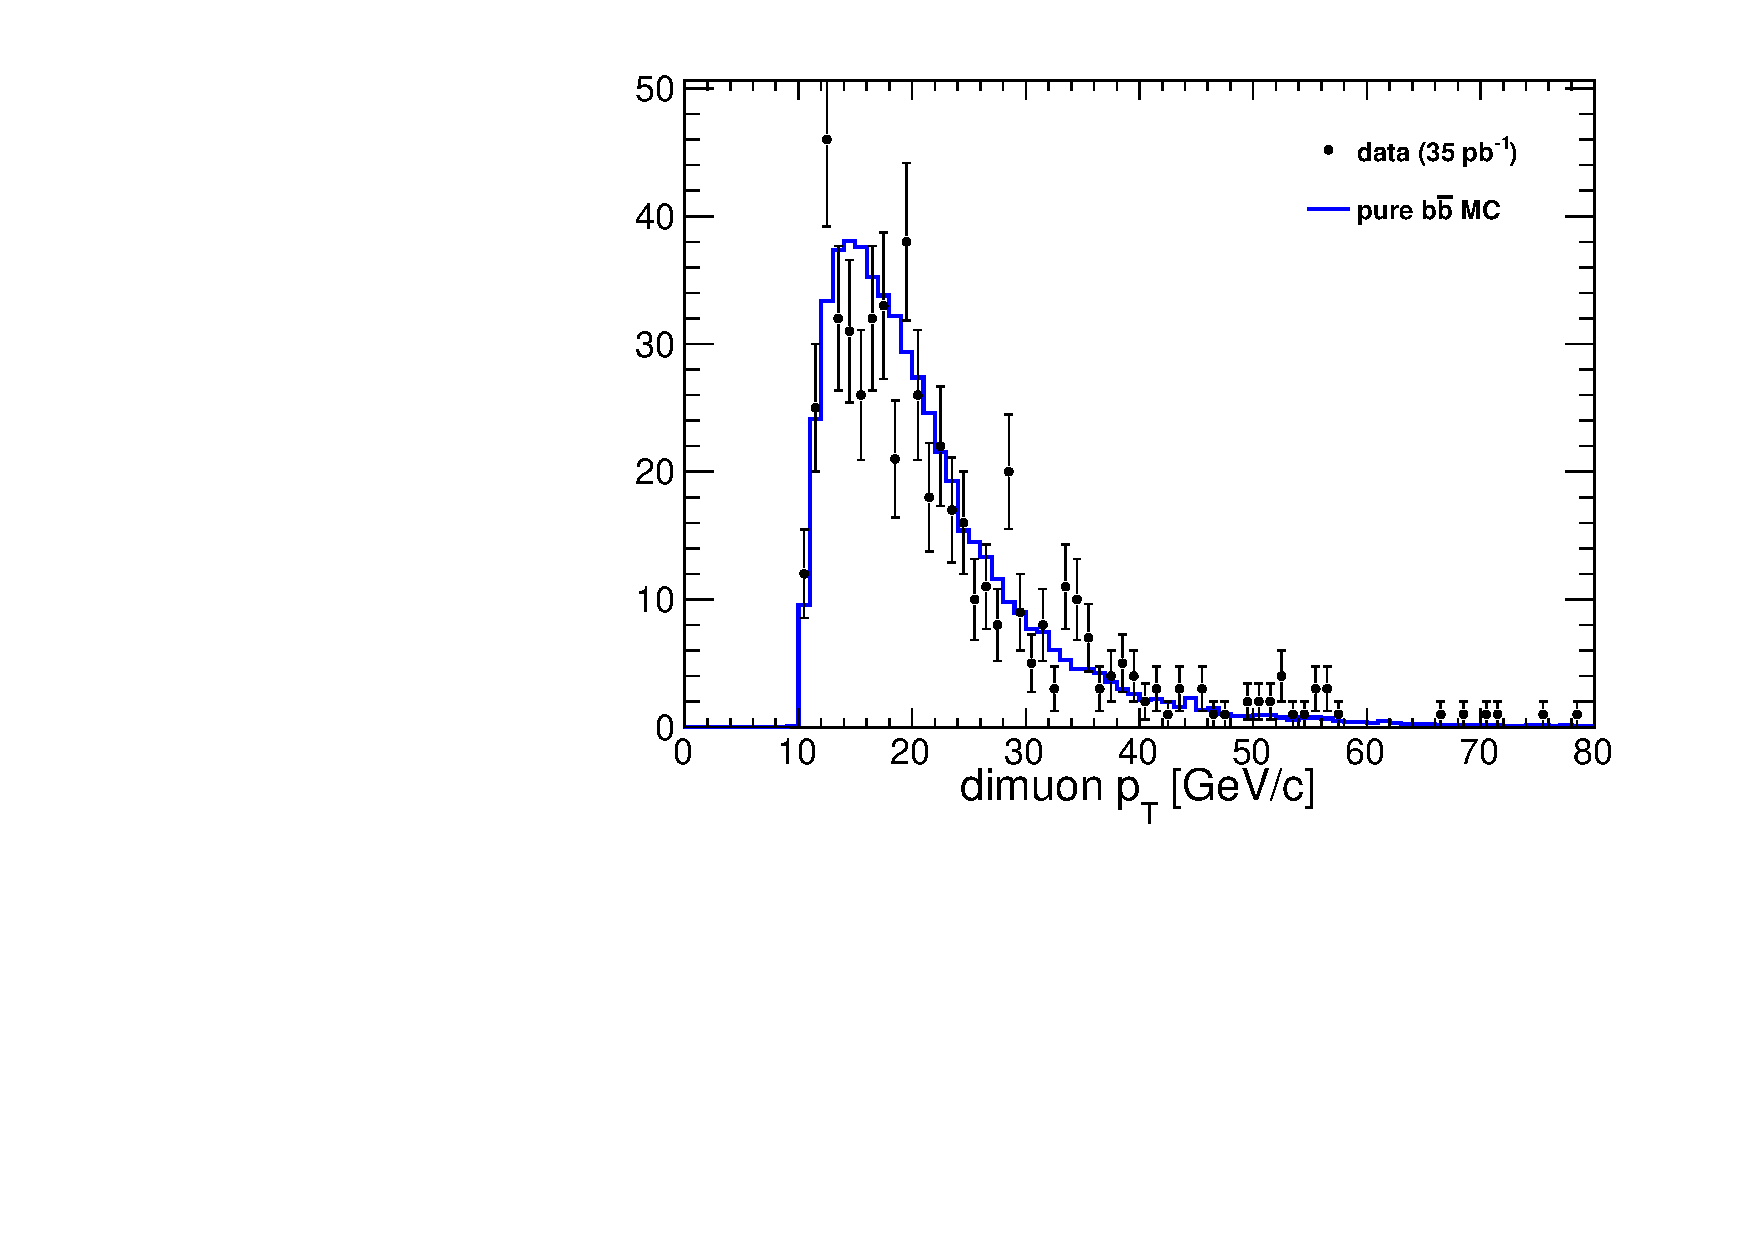
\includegraphics[width=0.33\linewidth]{dimuorphan_pt.pdf}
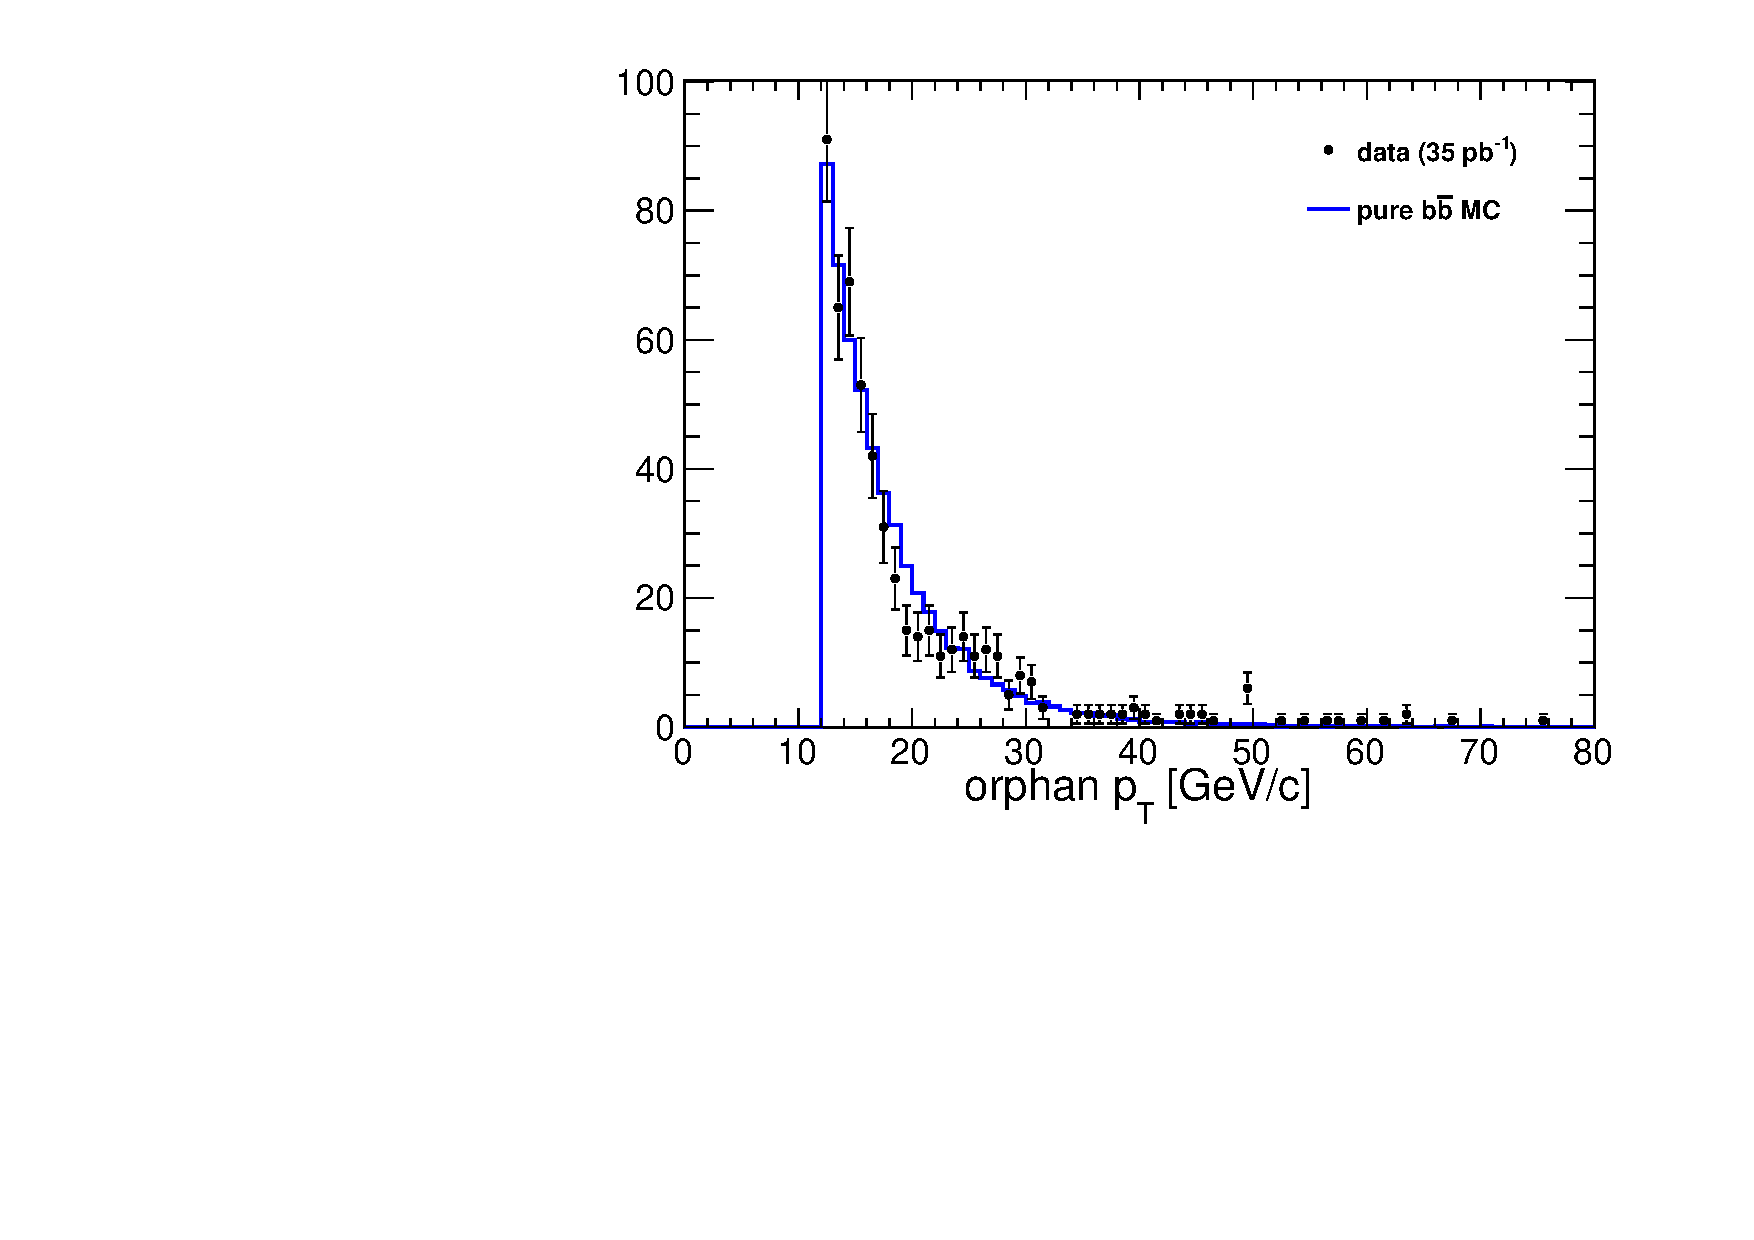
\includegraphics[width=0.33\linewidth]{dimuorphan_orphanpt.pdf} \hfill
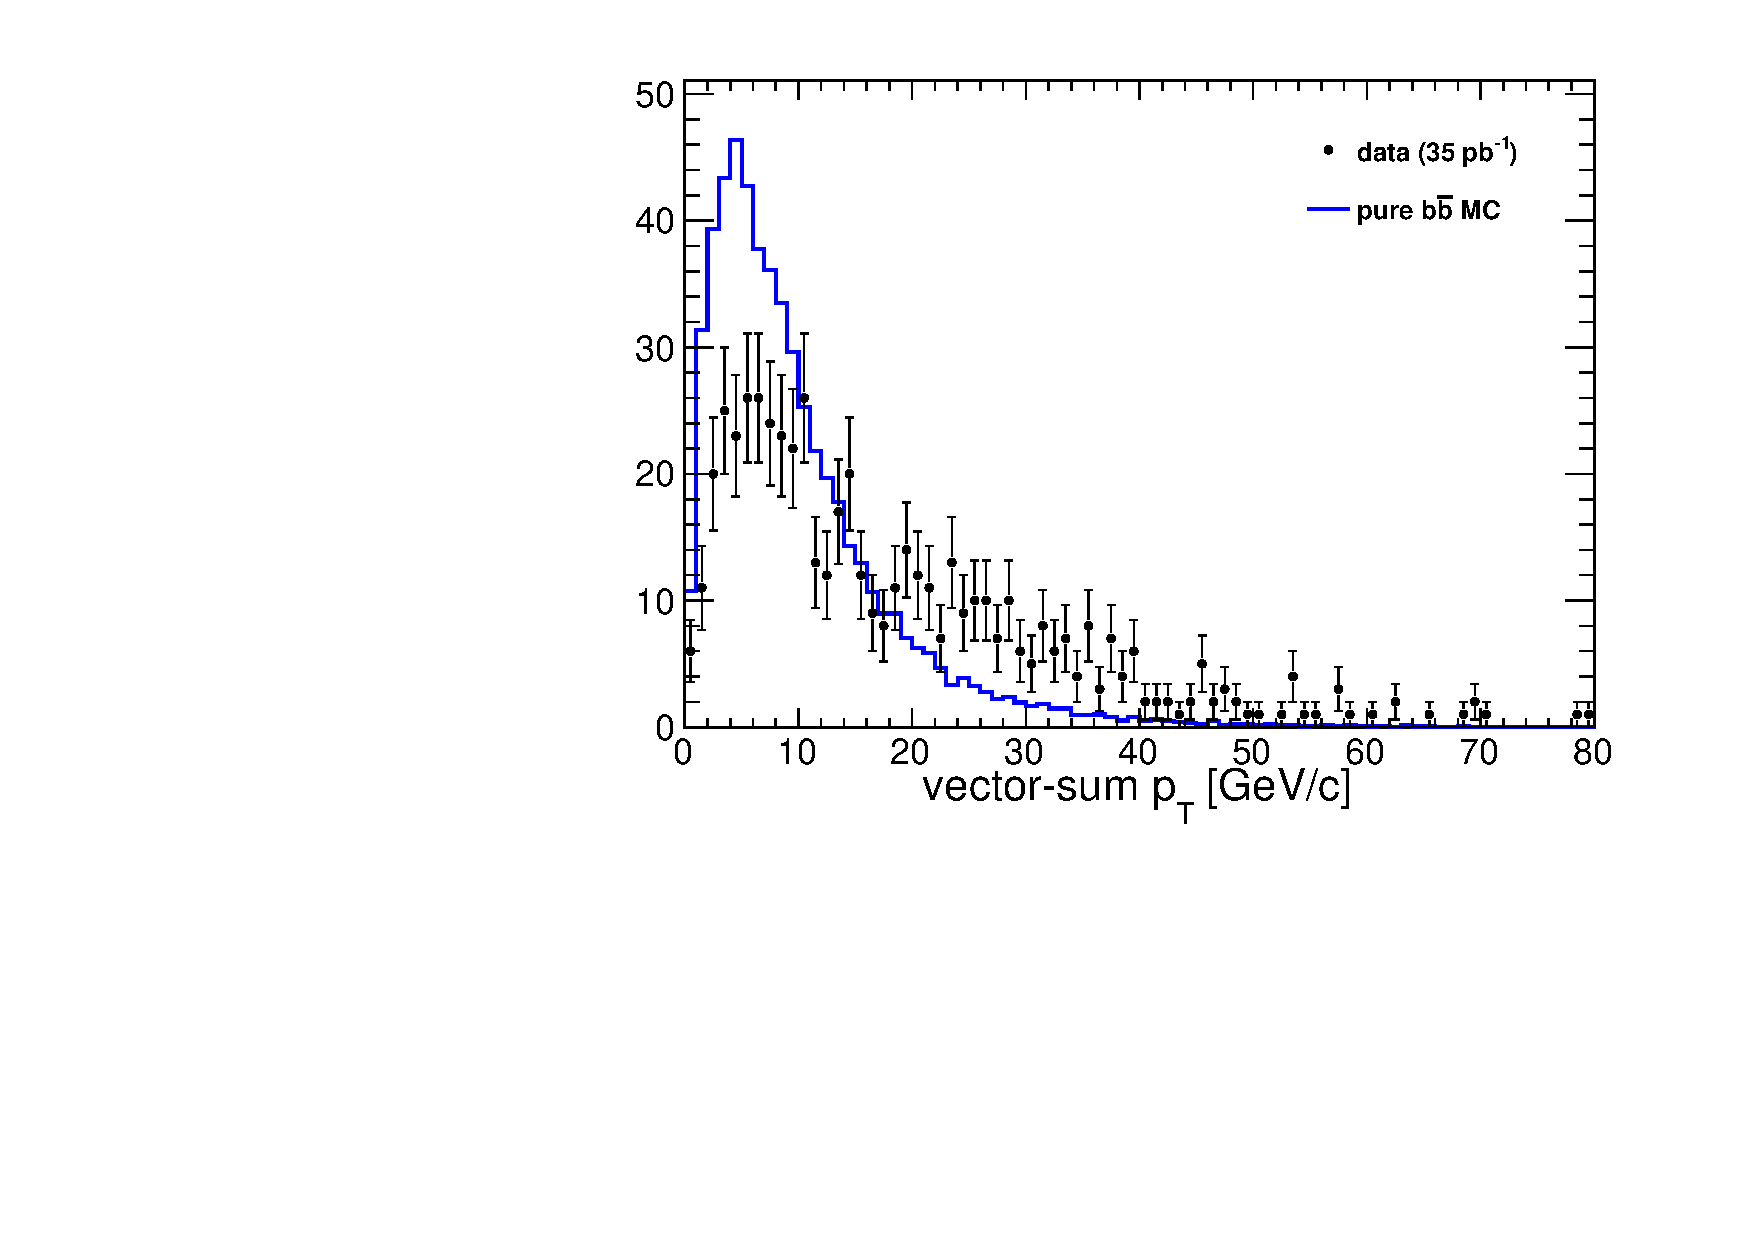
\includegraphics[width=0.33\linewidth]{dimuorphan_vectorsumpt.pdf}

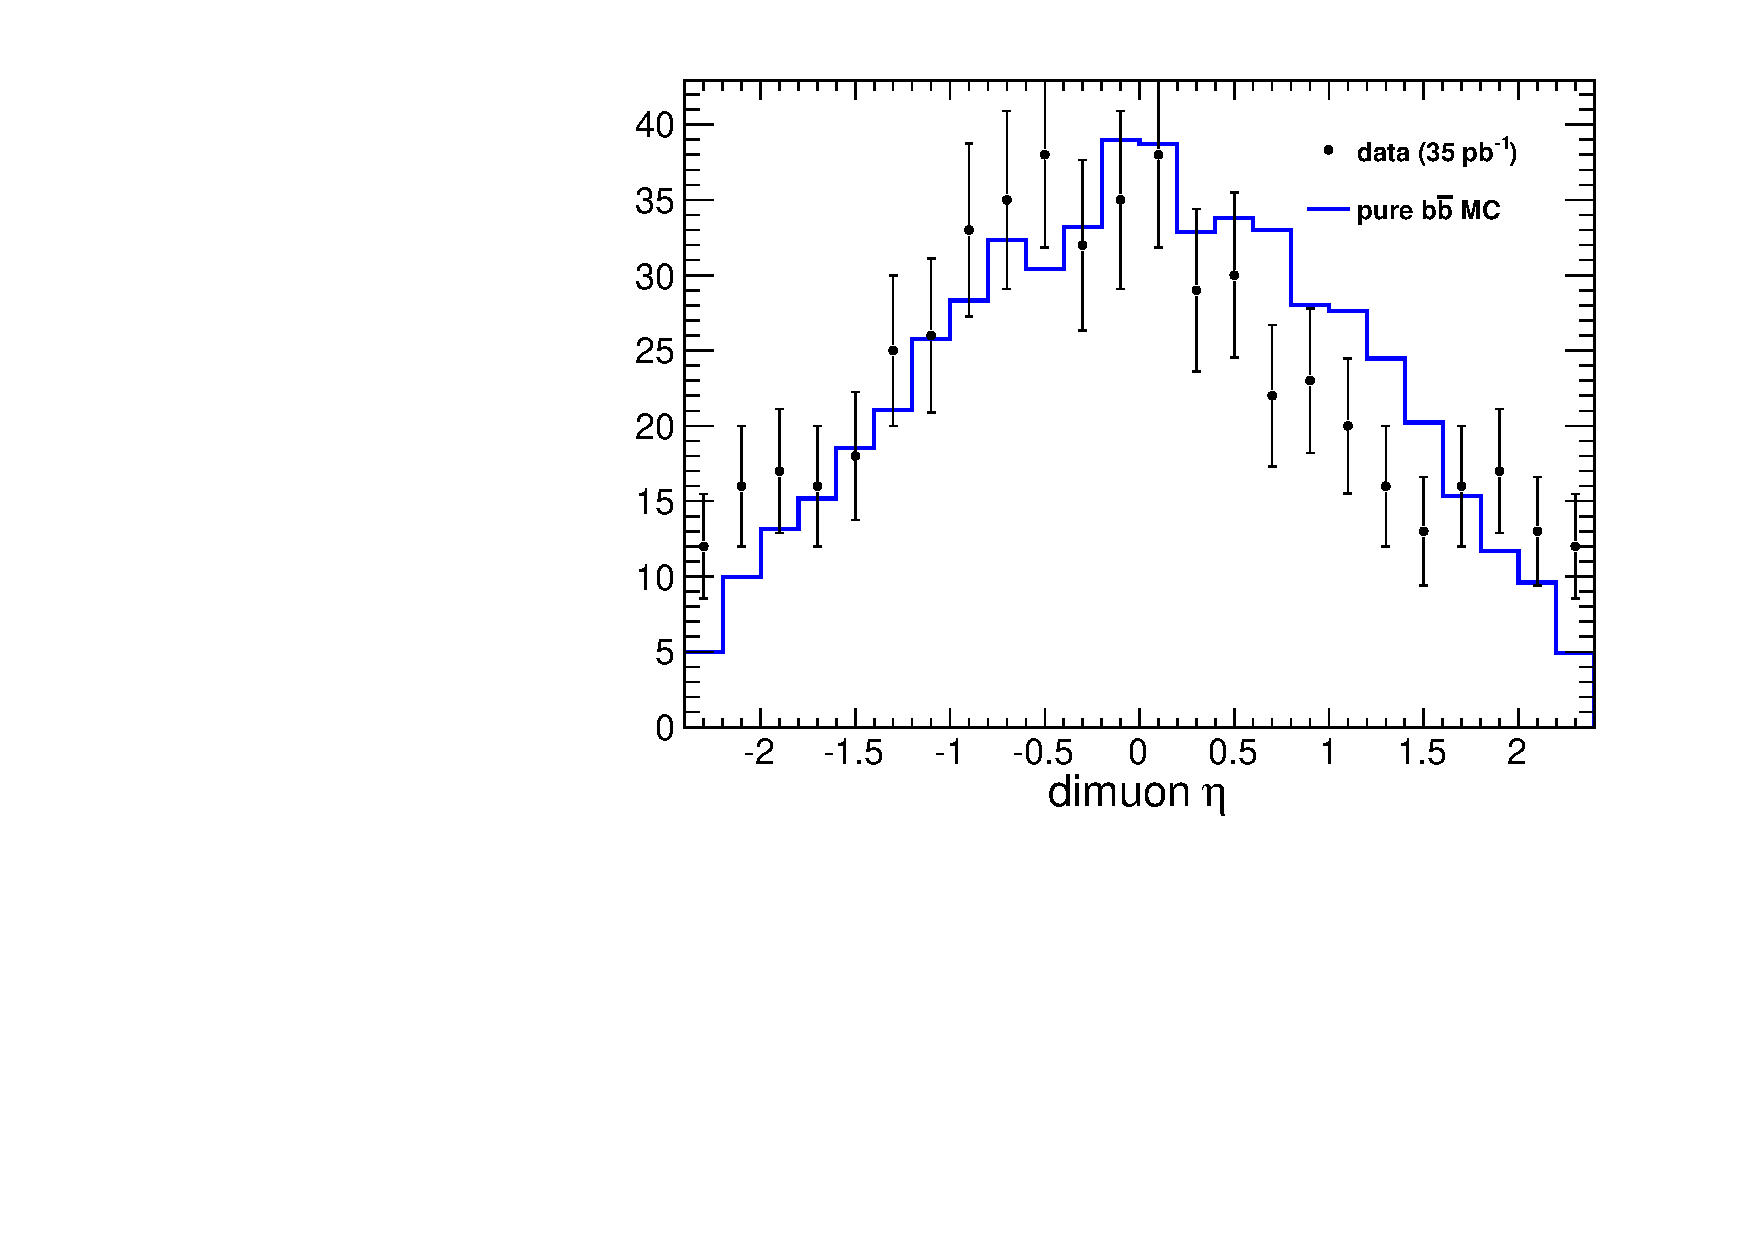
\includegraphics[width=0.33\linewidth]{dimuorphan_eta.pdf}
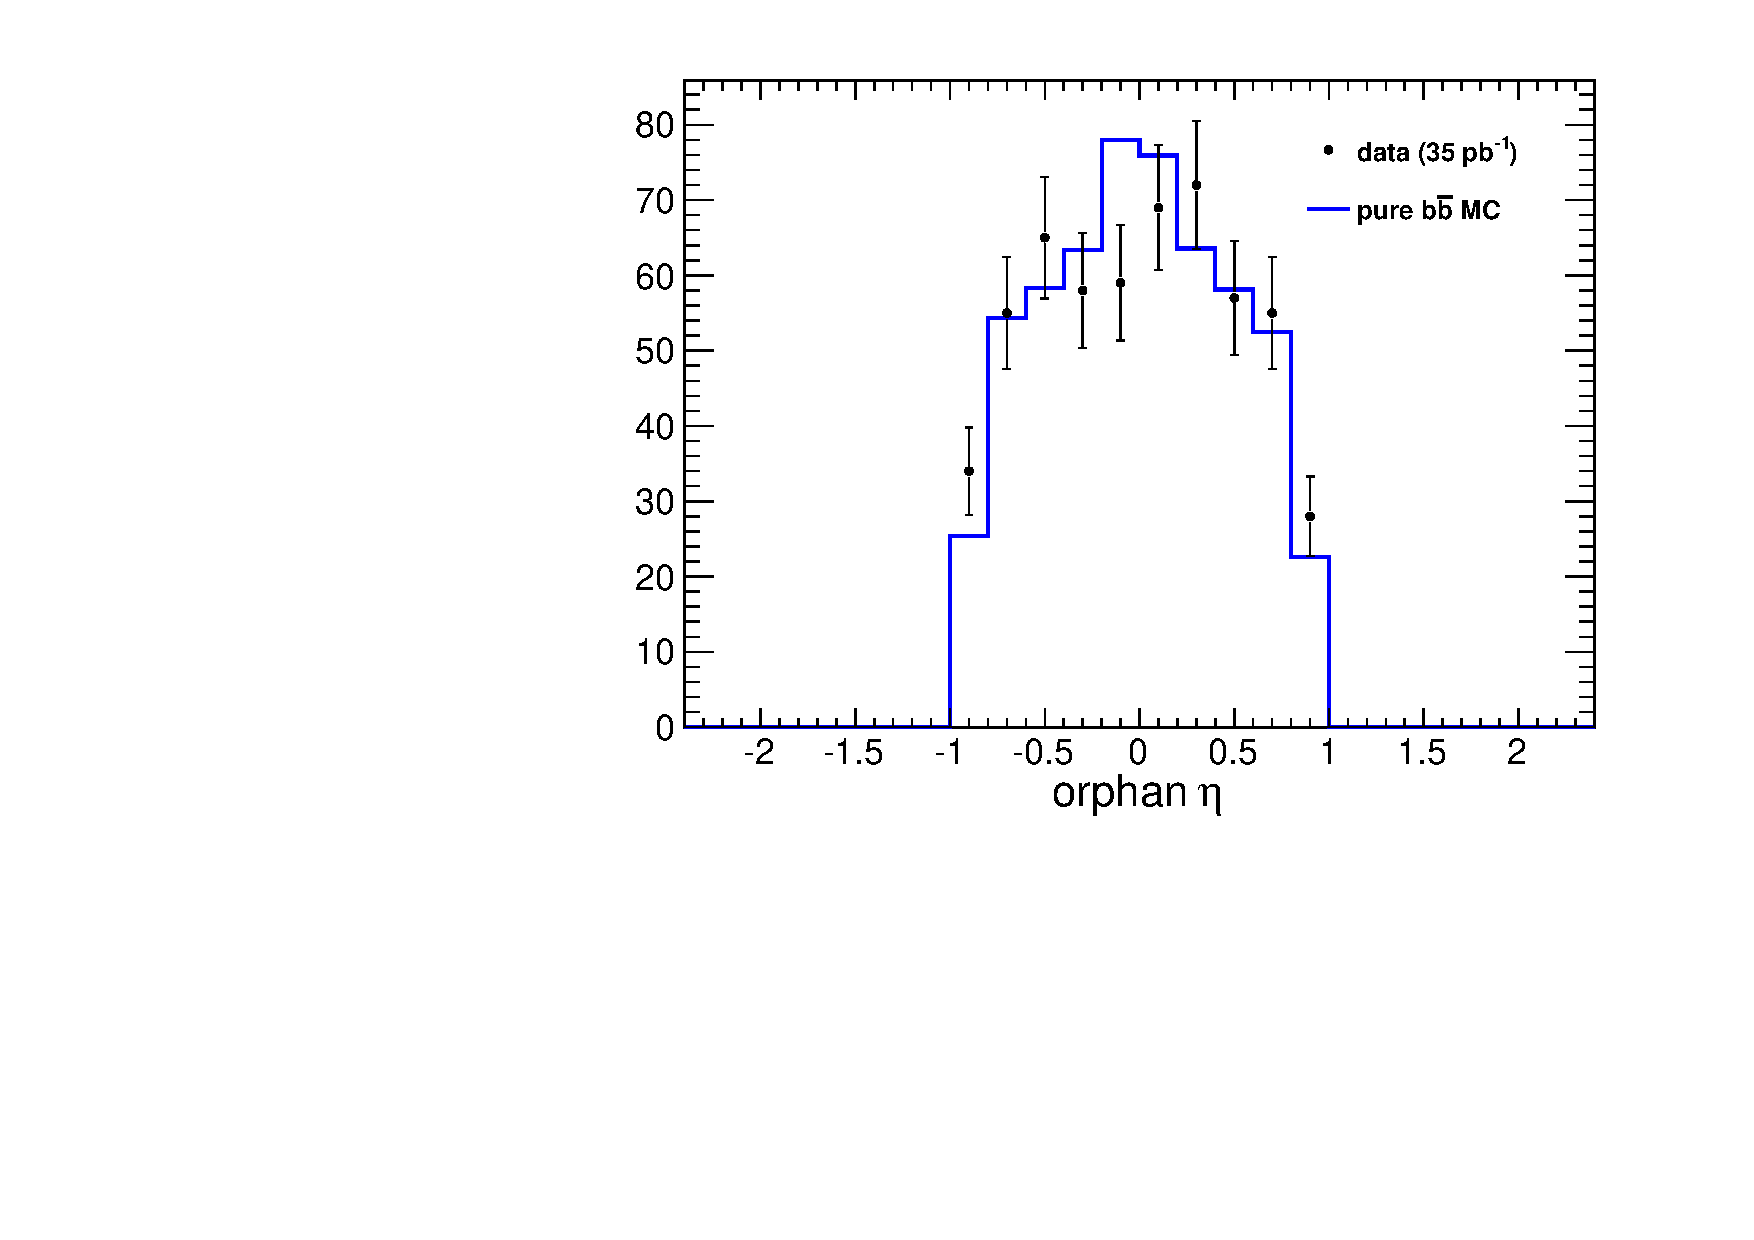
\includegraphics[width=0.33\linewidth]{dimuorphan_orphaneta.pdf}
\end{frame}

\begin{frame}
\frametitle{Diagnostic of $|\Delta\phi| < 1$ events}
\framesubtitle{$|\Delta\phi| < 1$ when the dimuon and the orphan are nearly collinear: \\ something that never happens in the $b\bar{b}$ MC}

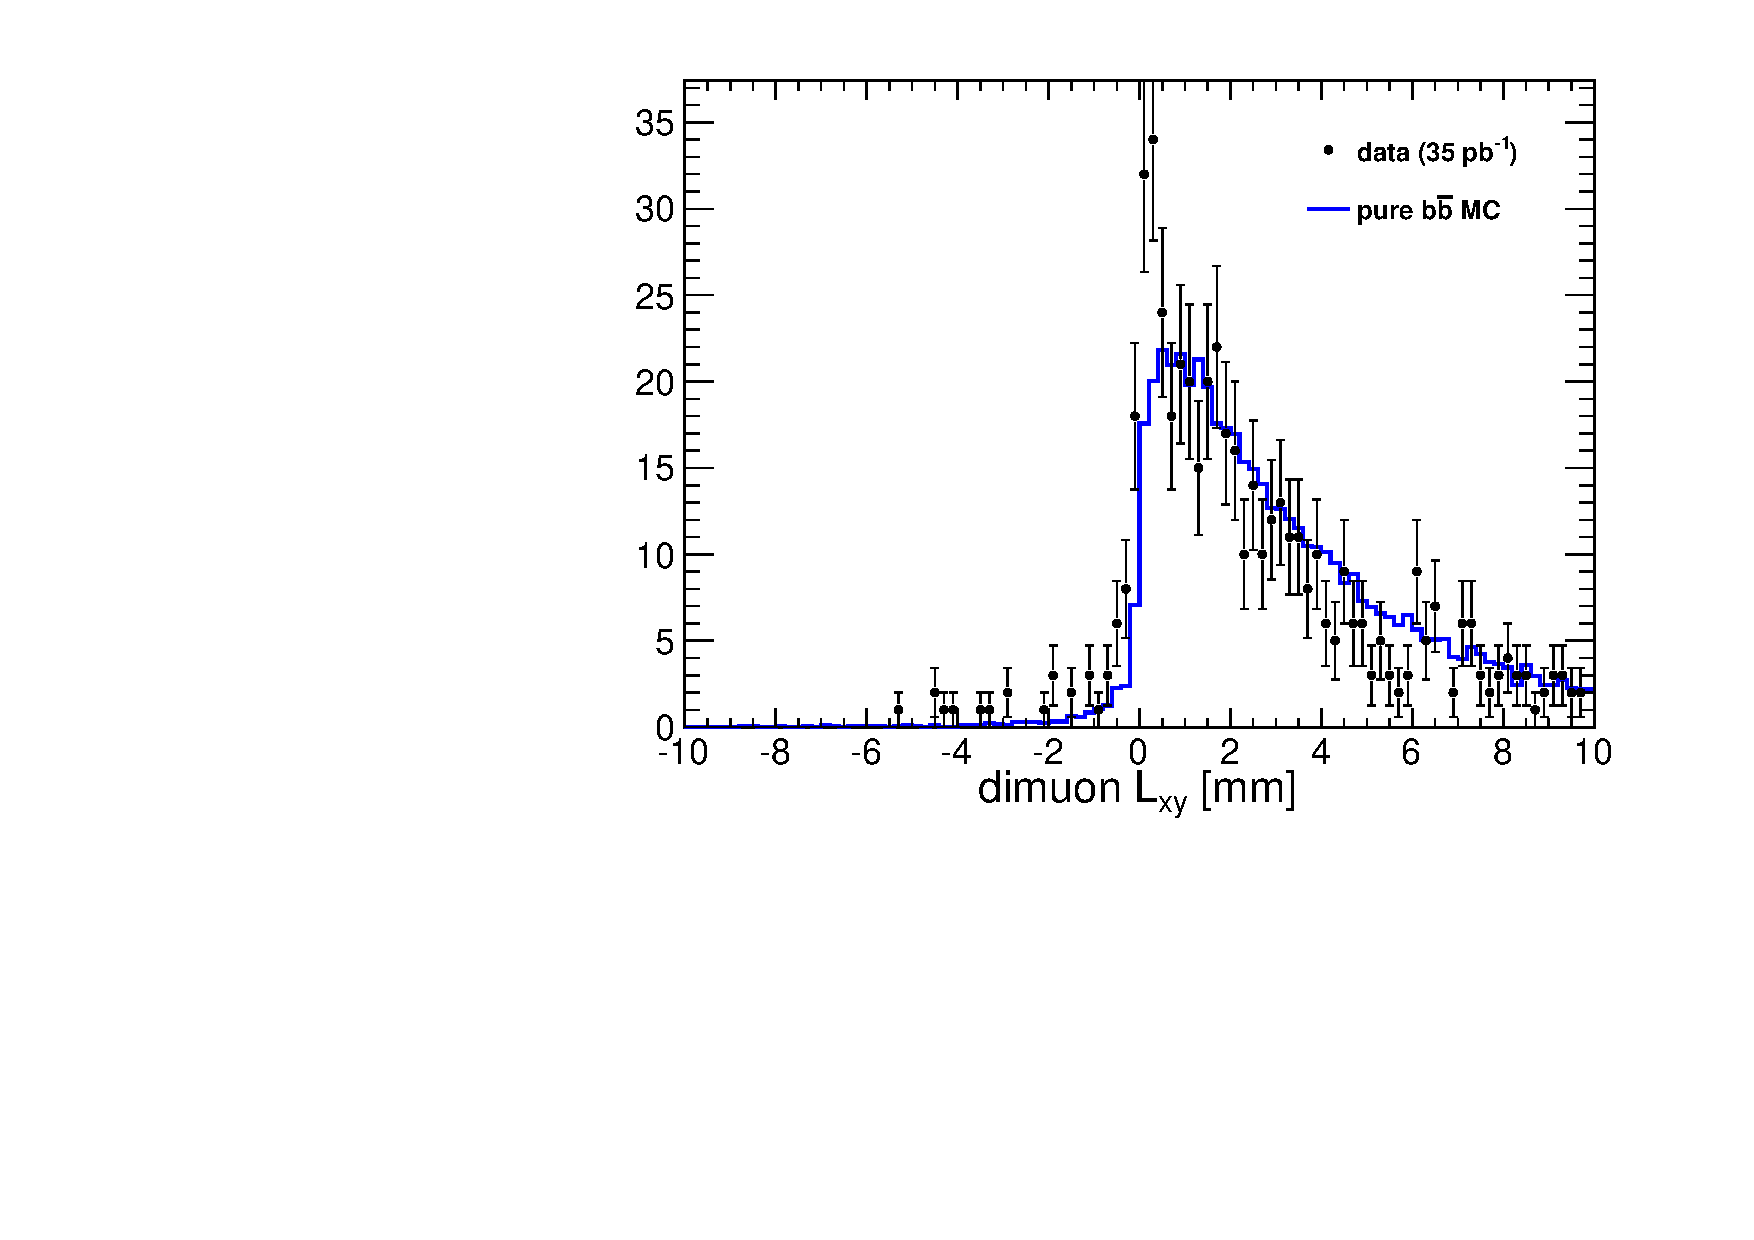
\includegraphics[width=0.5\linewidth]{dimuorphan_lxy.pdf}
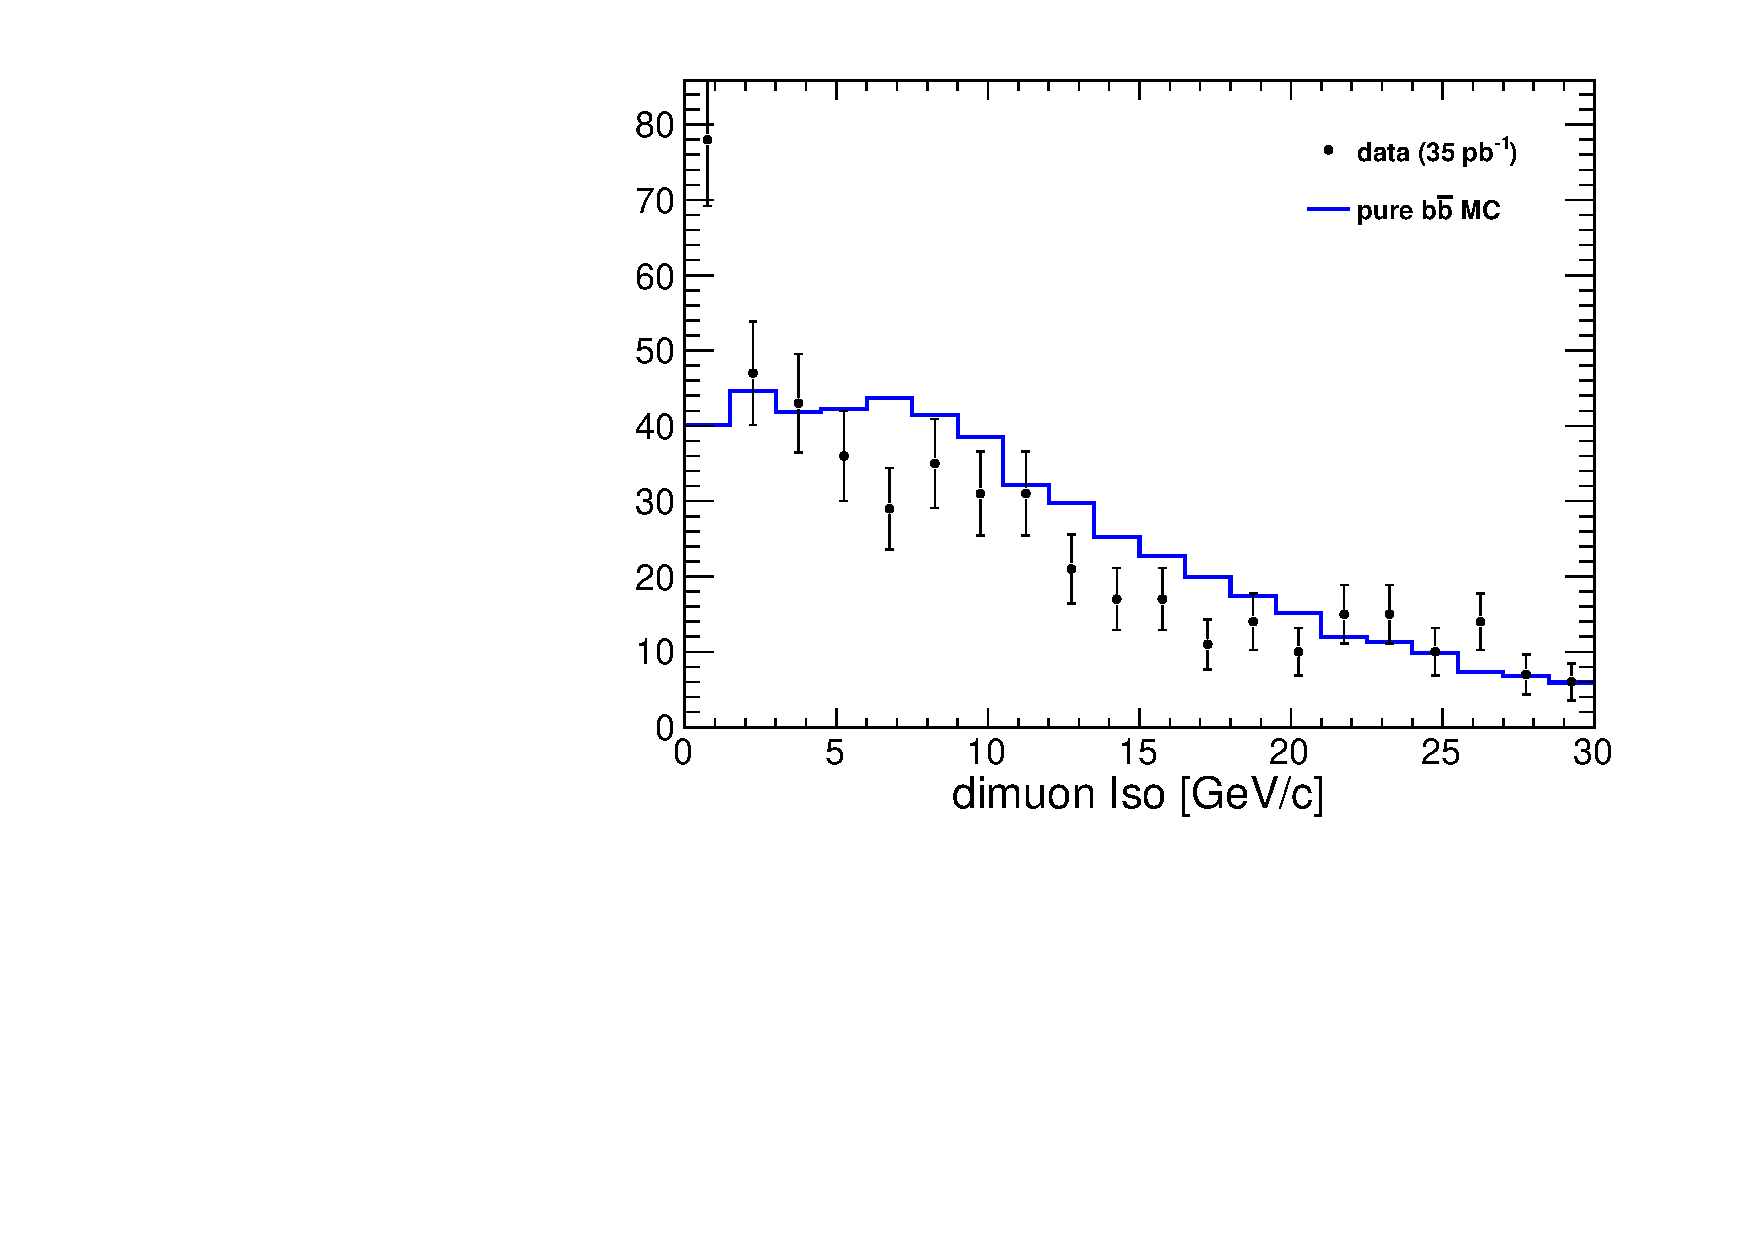
\includegraphics[width=0.5\linewidth]{dimuorphan_iso.pdf}

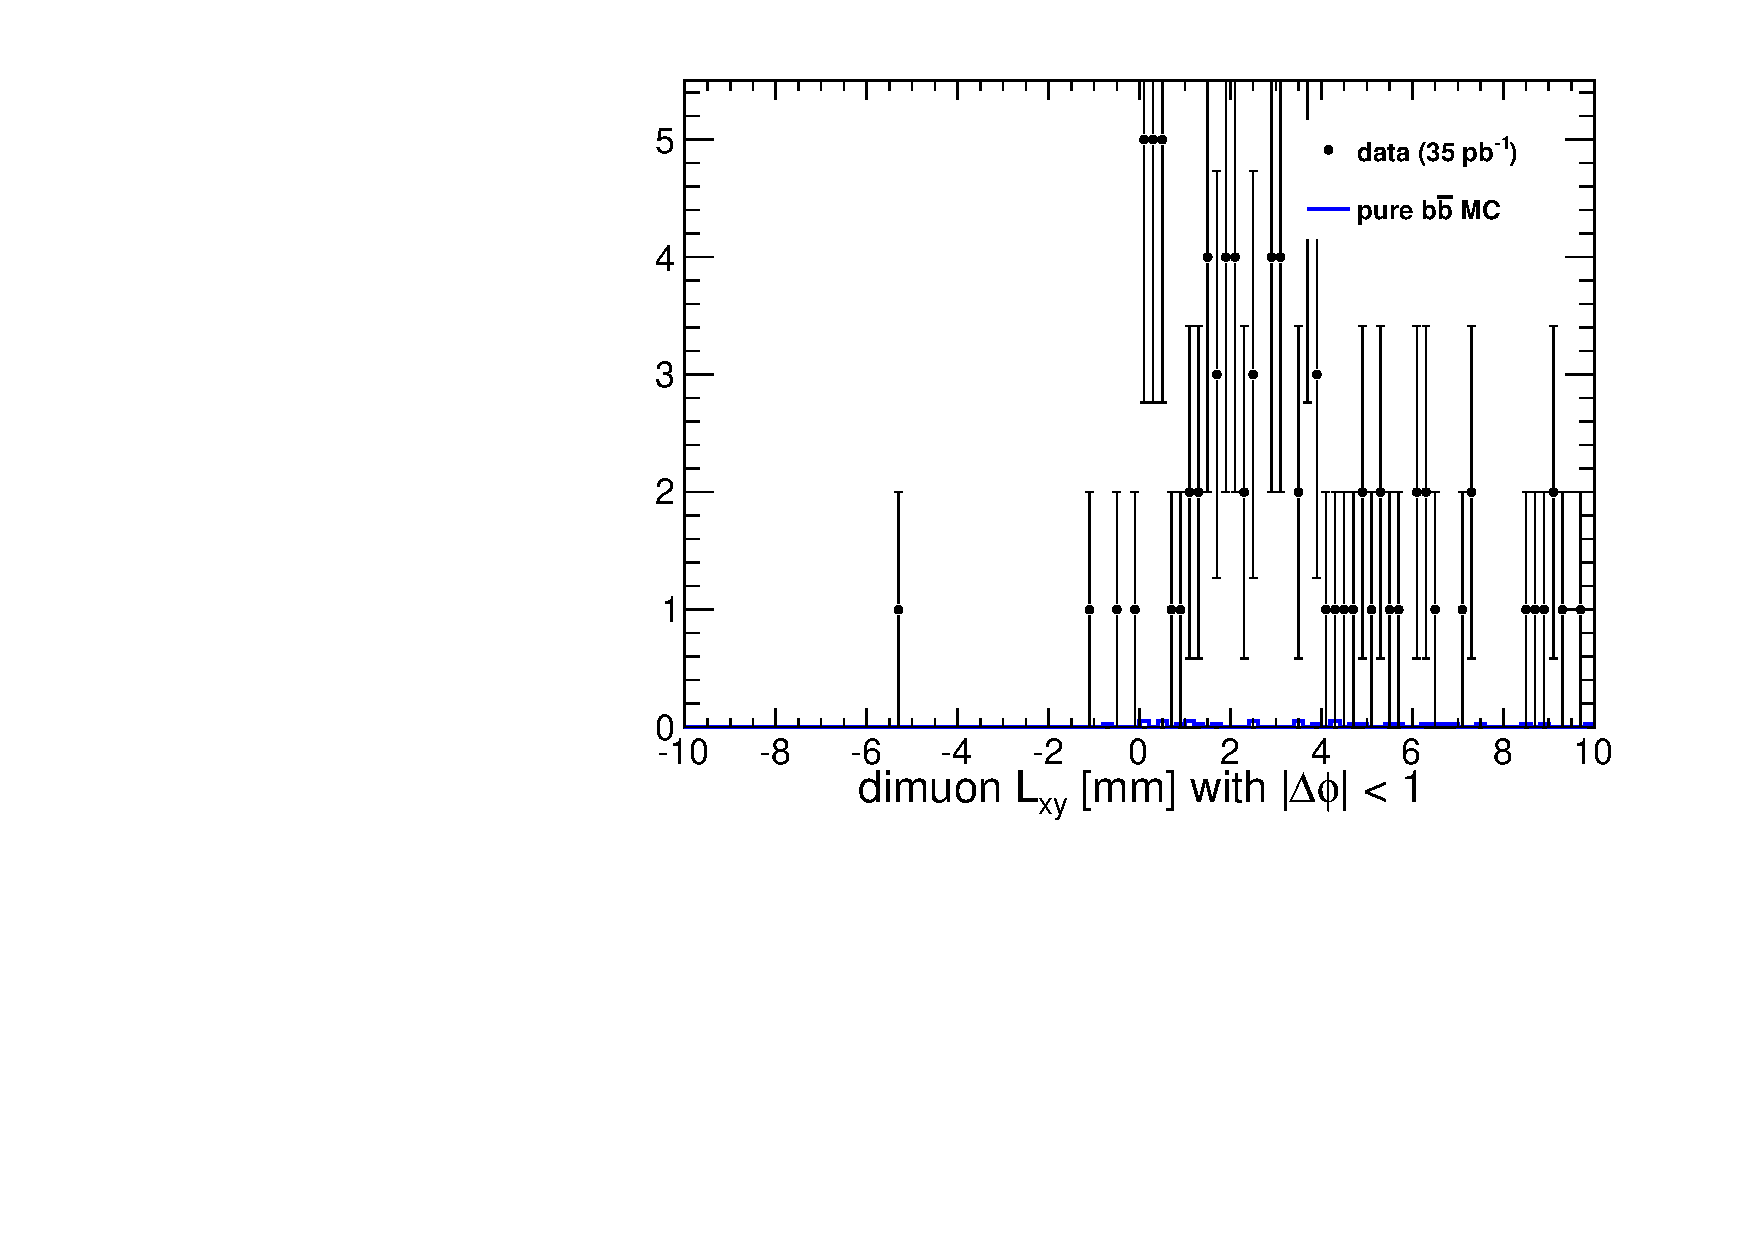
\includegraphics[width=0.5\linewidth]{dimuorphan_lxy_collinear.pdf}
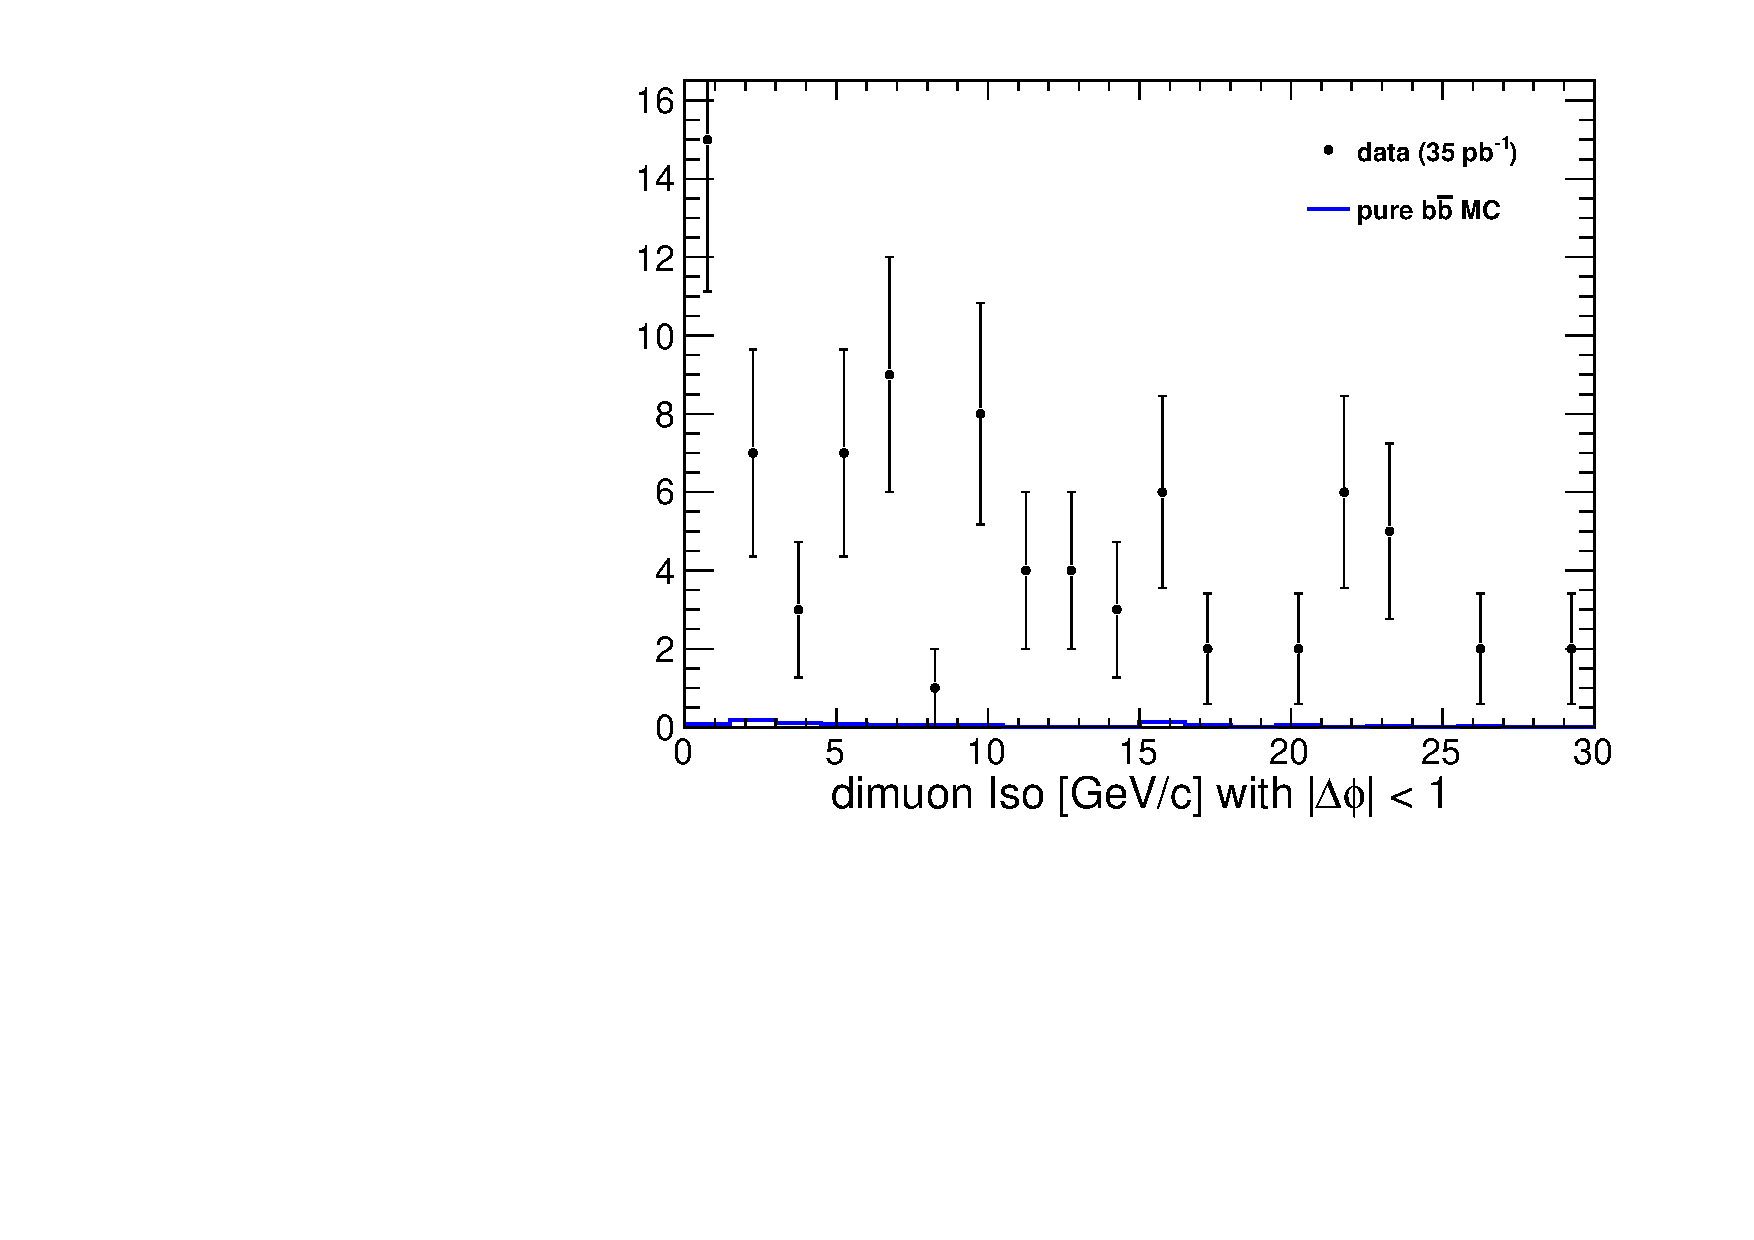
\includegraphics[width=0.5\linewidth]{dimuorphan_iso_collinear.pdf}
\end{frame}

\begin{frame}
\frametitle{Diagnostic of $|\Delta\phi| < 1$ events}
\framesubtitle{$|\Delta\phi| < 1$ when the dimuon and the orphan are nearly collinear: \\ something that never happens in the $b\bar{b}$ MC}

Muon quality plots for the orphan

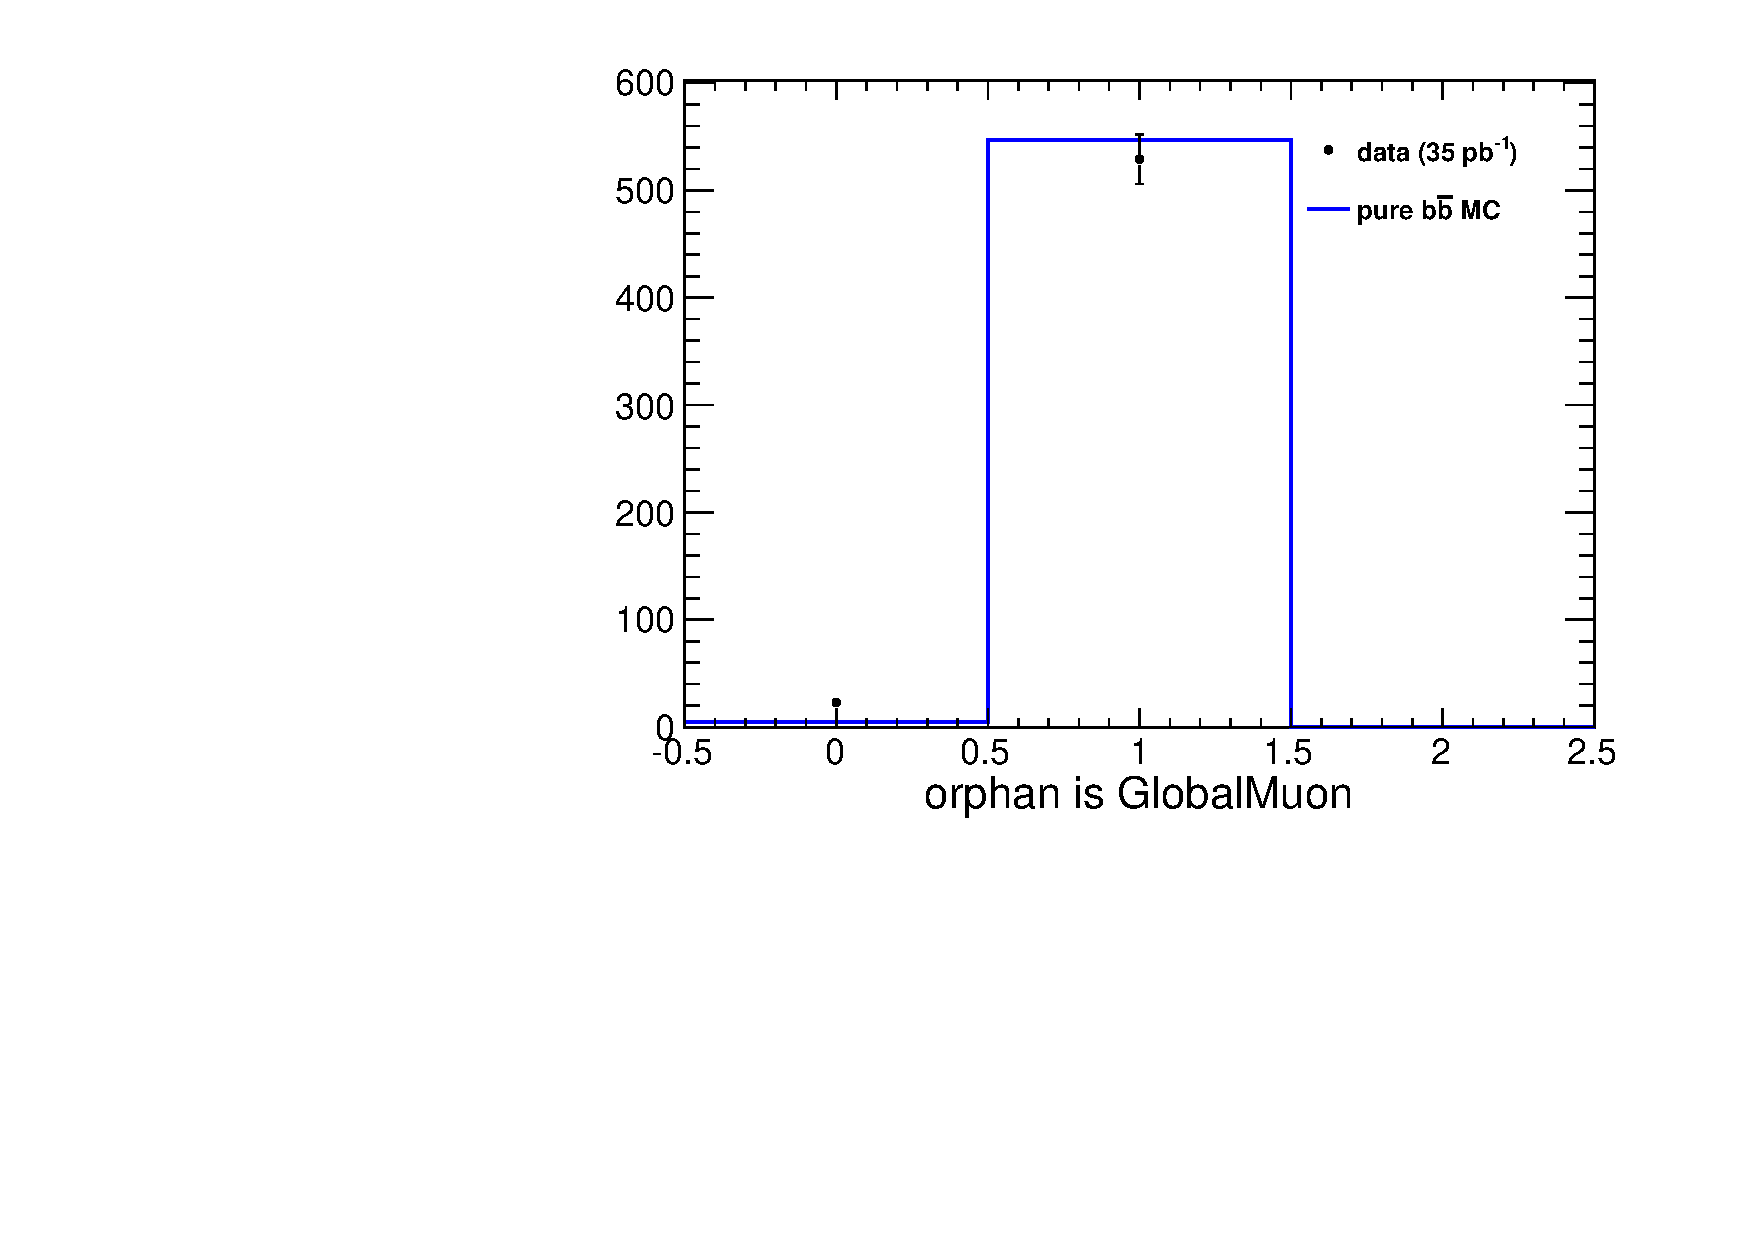
\includegraphics[width=0.45\linewidth]{dimuorphan_isglobal.pdf}
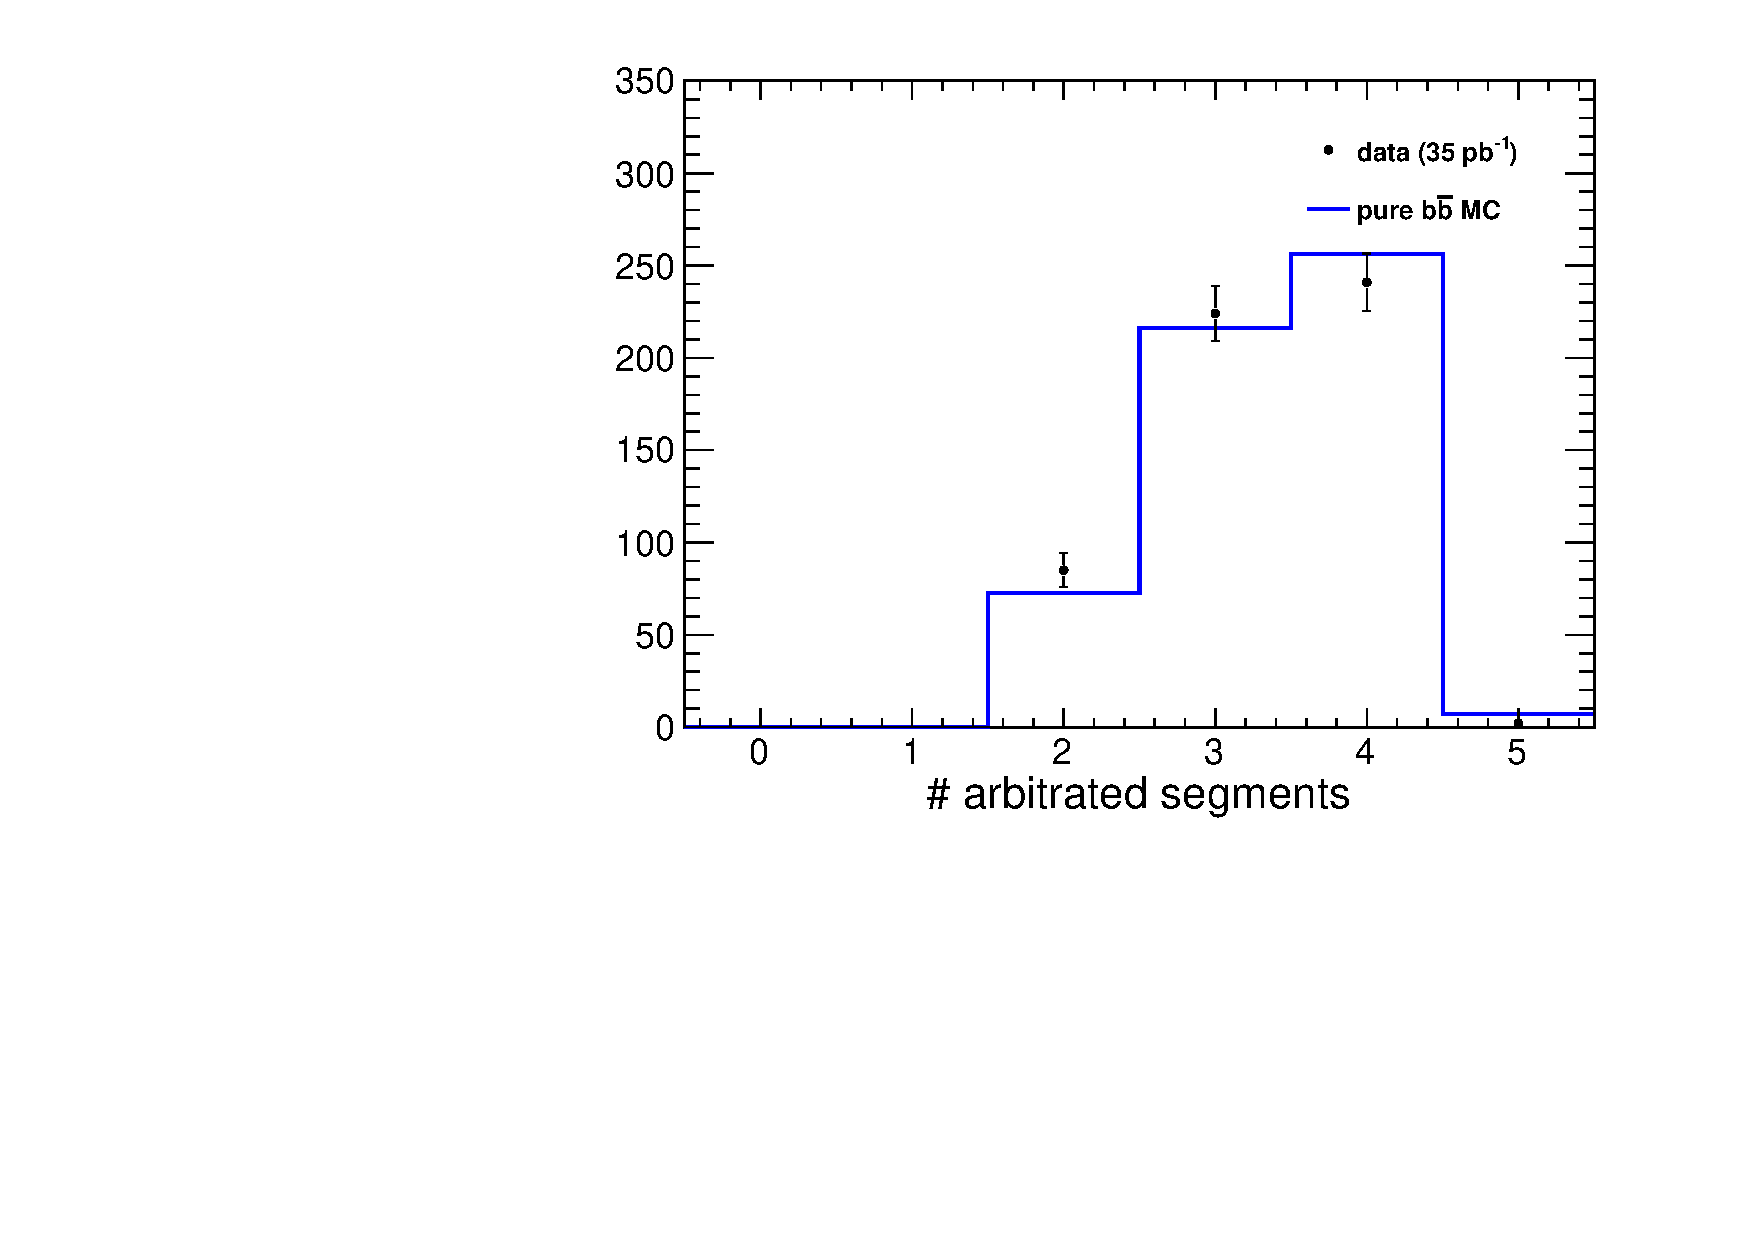
\includegraphics[width=0.45\linewidth]{dimuorphan_orphanmatches.pdf}

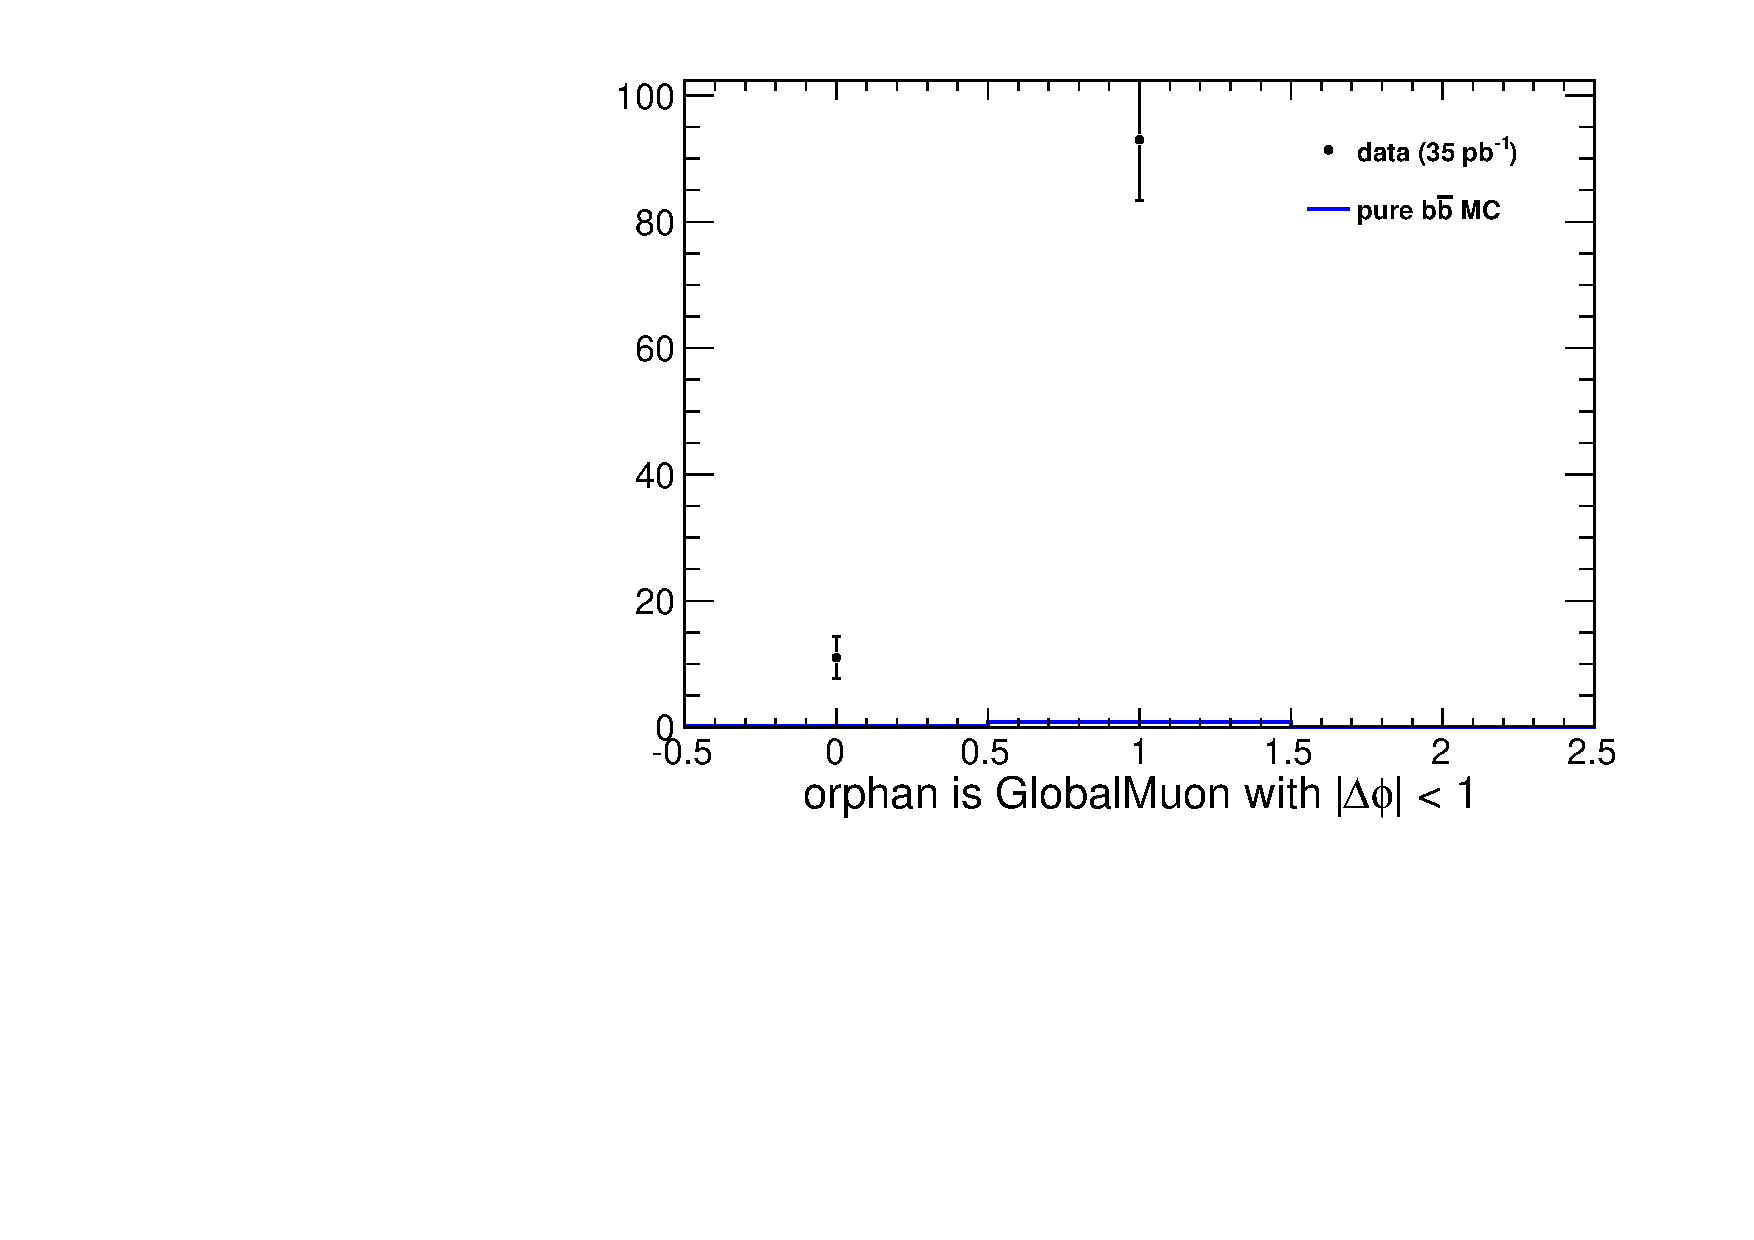
\includegraphics[width=0.45\linewidth]{dimuorphan_isglobal_collinear.pdf}
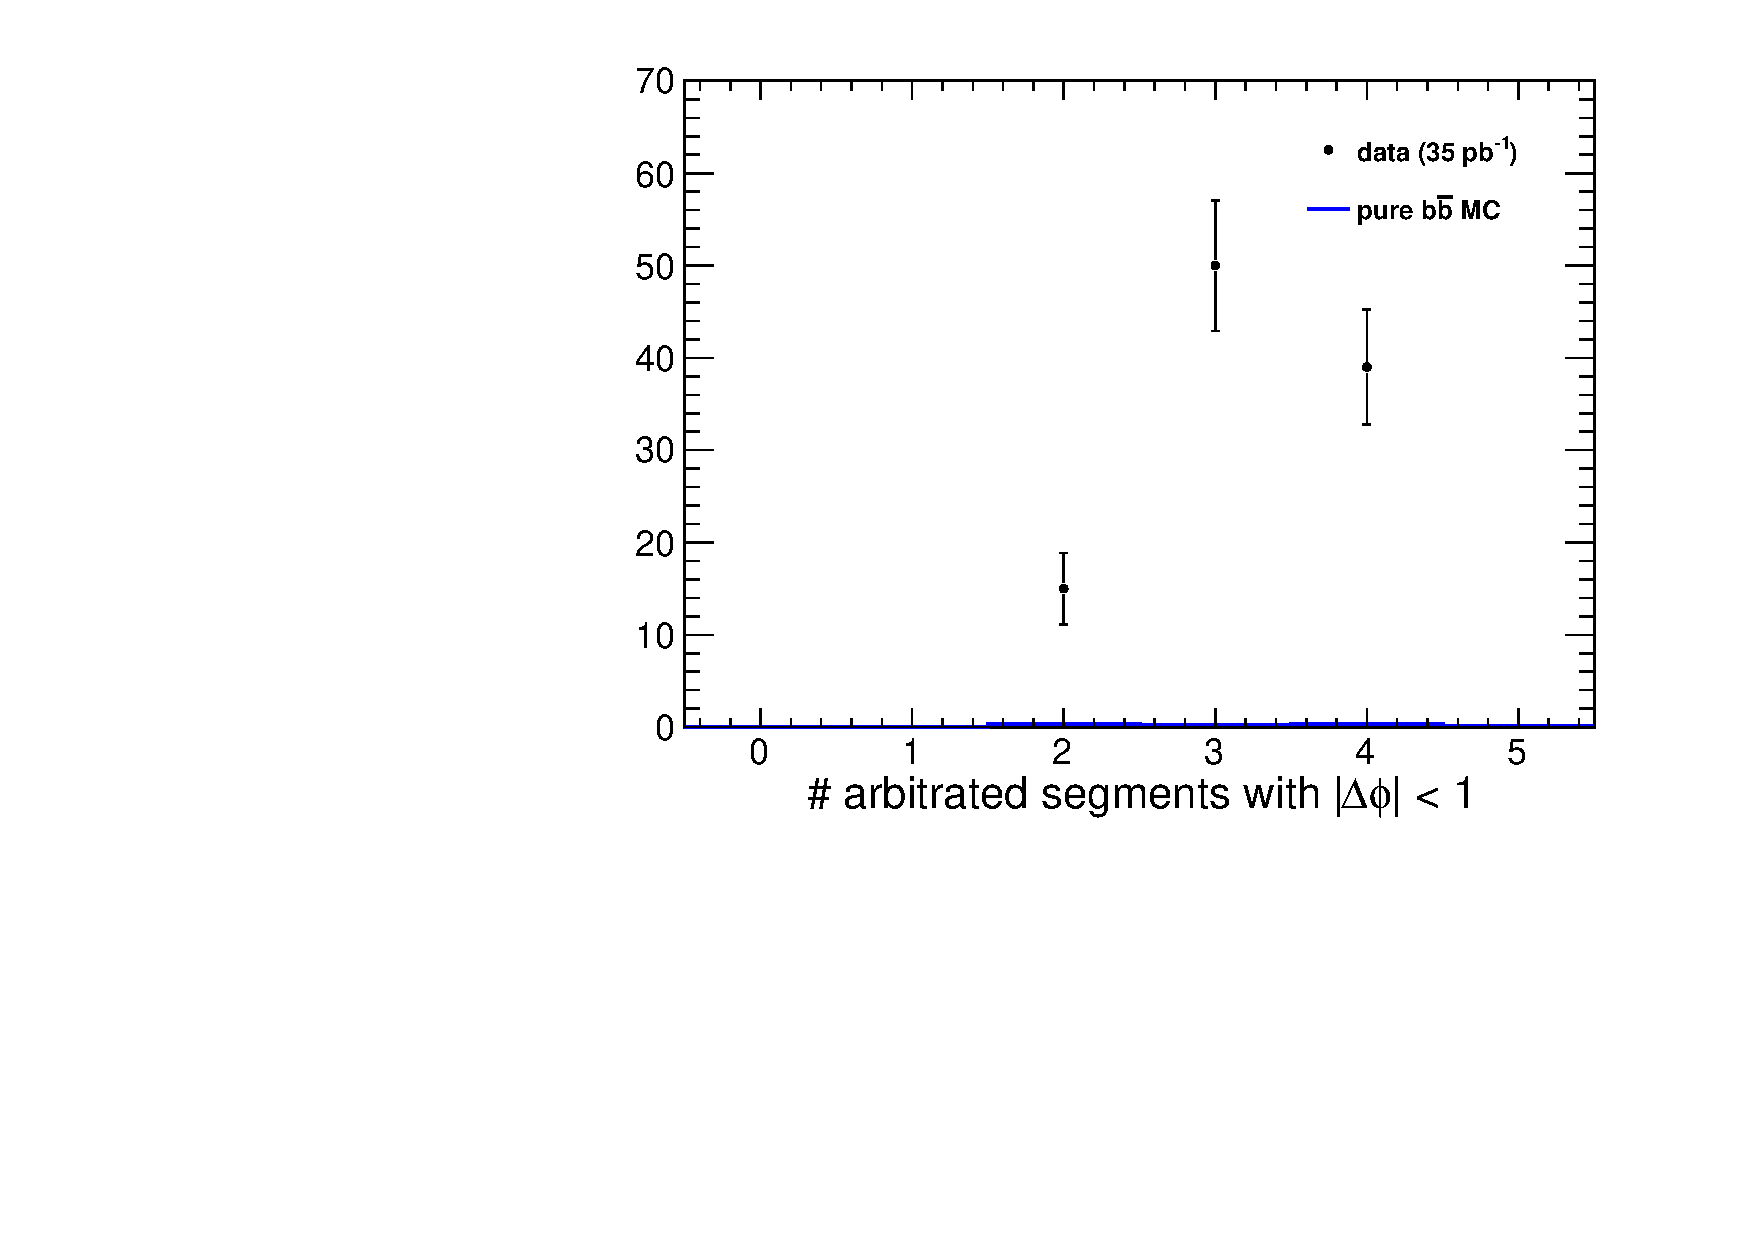
\includegraphics[width=0.45\linewidth]{dimuorphan_orphanmatches_collinear.pdf}
\end{frame}

\begin{frame}
\frametitle{Diagnostic of $|\Delta\phi| < 1$ events}
\framesubtitle{$|\Delta\phi| < 1$ when the dimuon and the orphan are nearly collinear: \\ something that never happens in the $b\bar{b}$ MC}

Tracker-track quality plots for the orphan

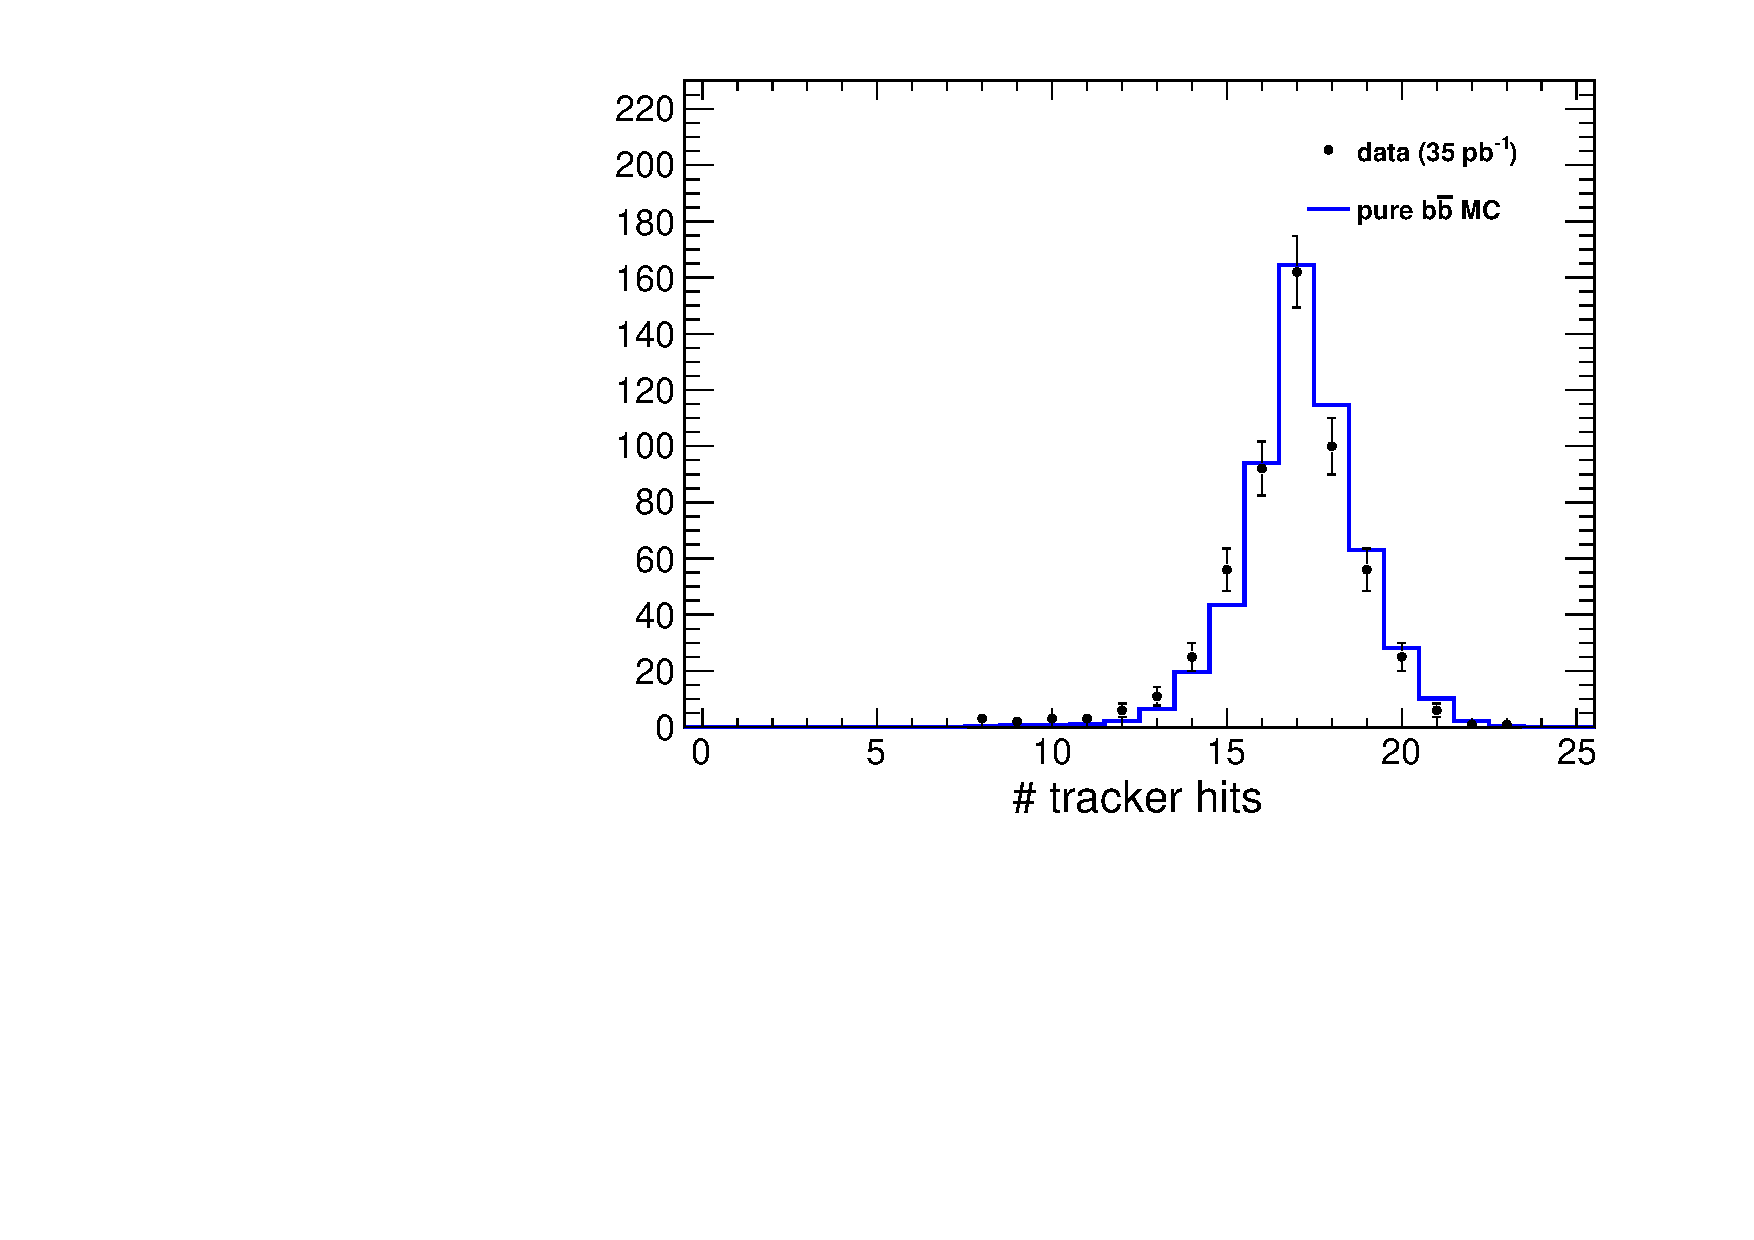
\includegraphics[width=0.43\linewidth]{dimuorphan_orphanhits.pdf}
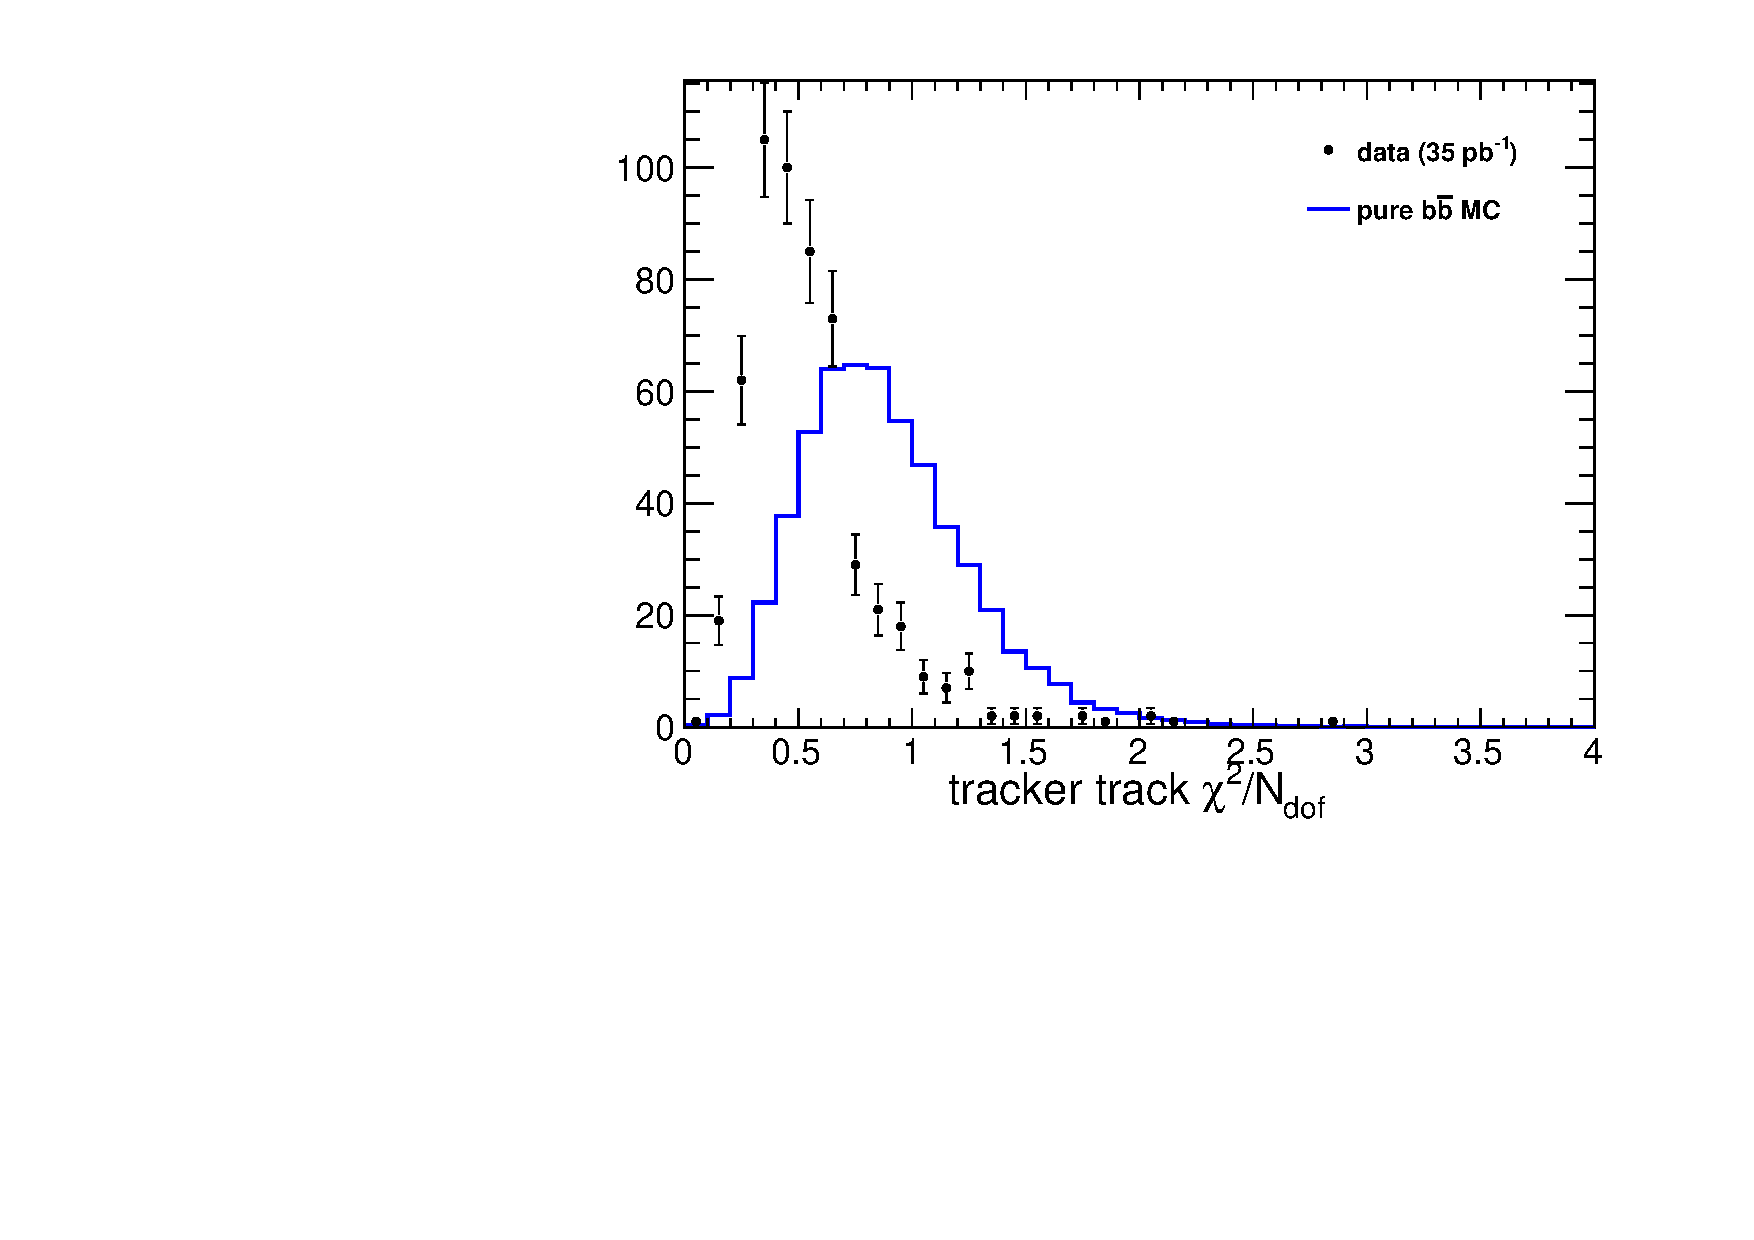
\includegraphics[width=0.43\linewidth]{dimuorphan_orphanchi2.pdf}

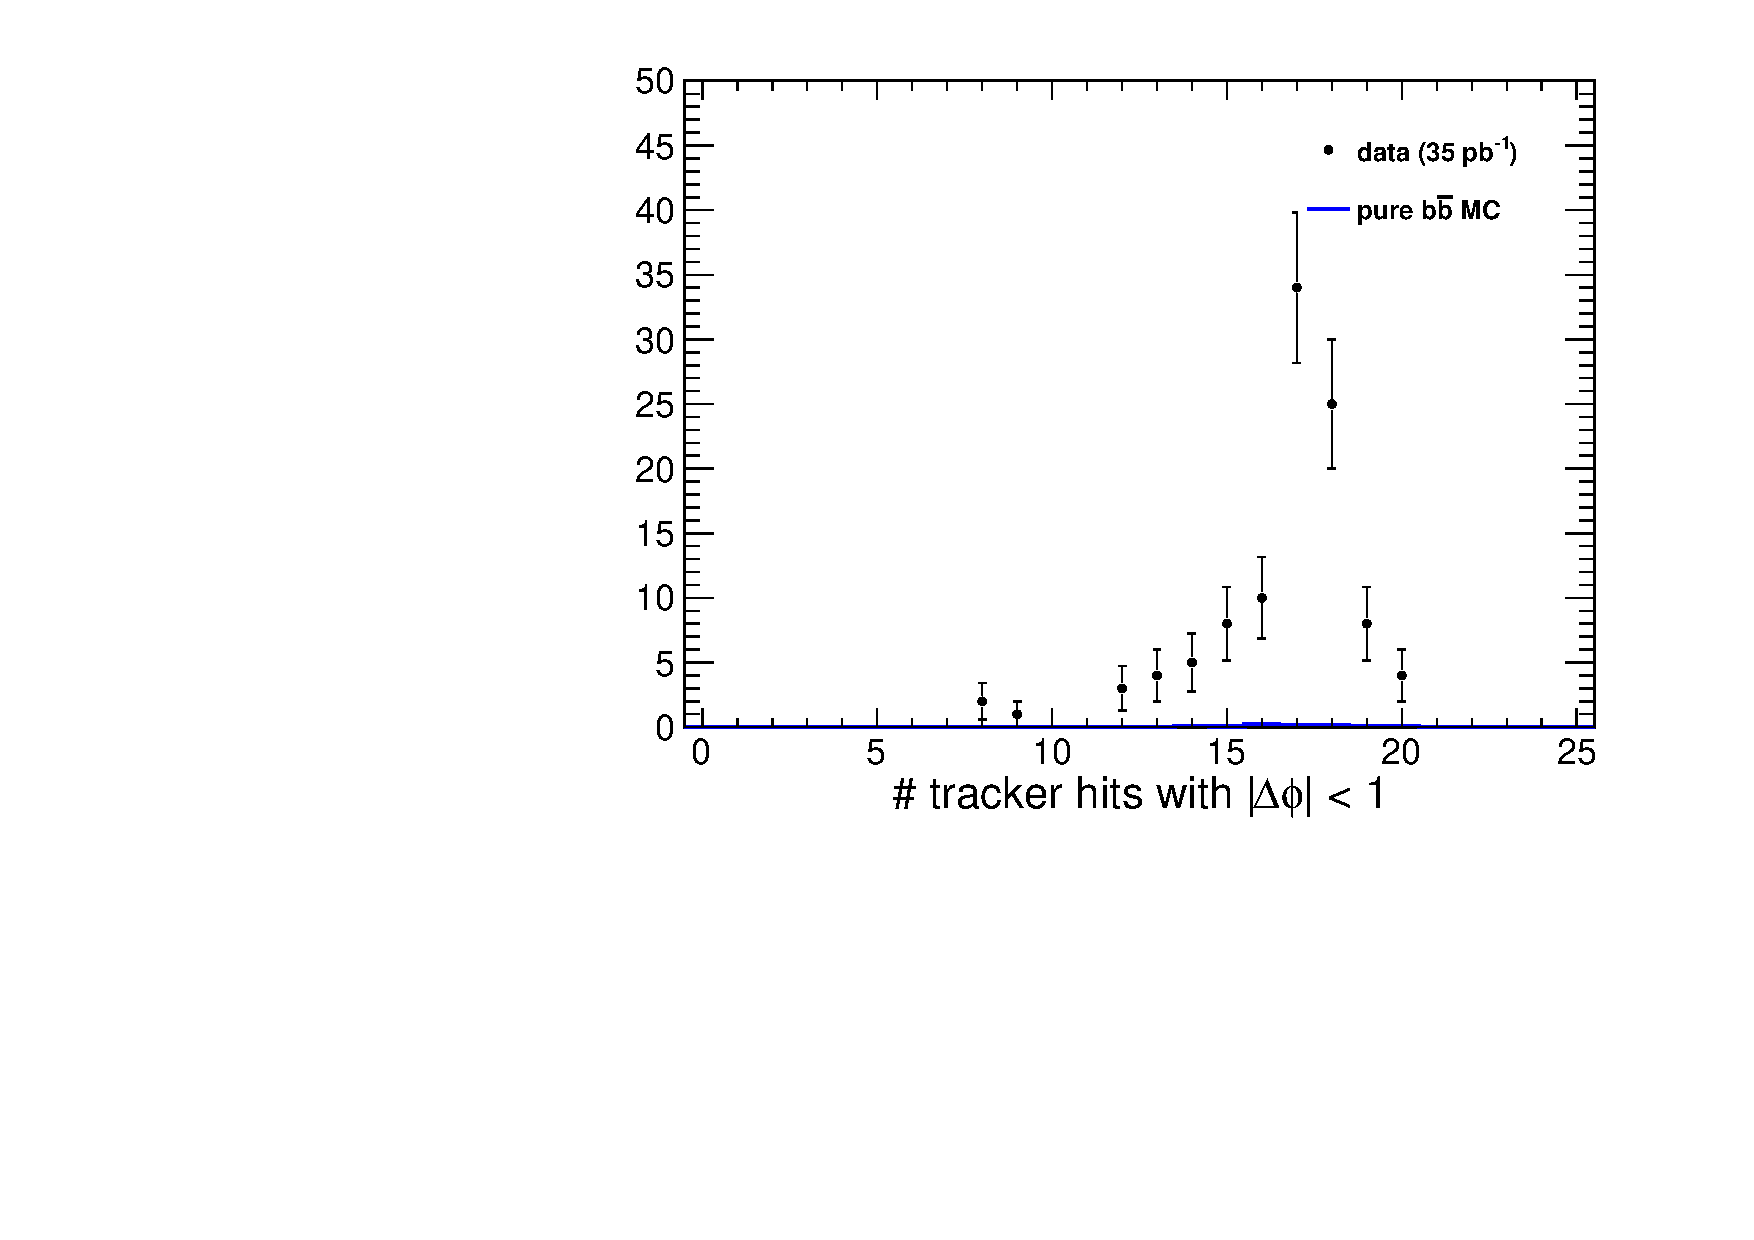
\includegraphics[width=0.43\linewidth]{dimuorphan_orphanhits_collinear.pdf}
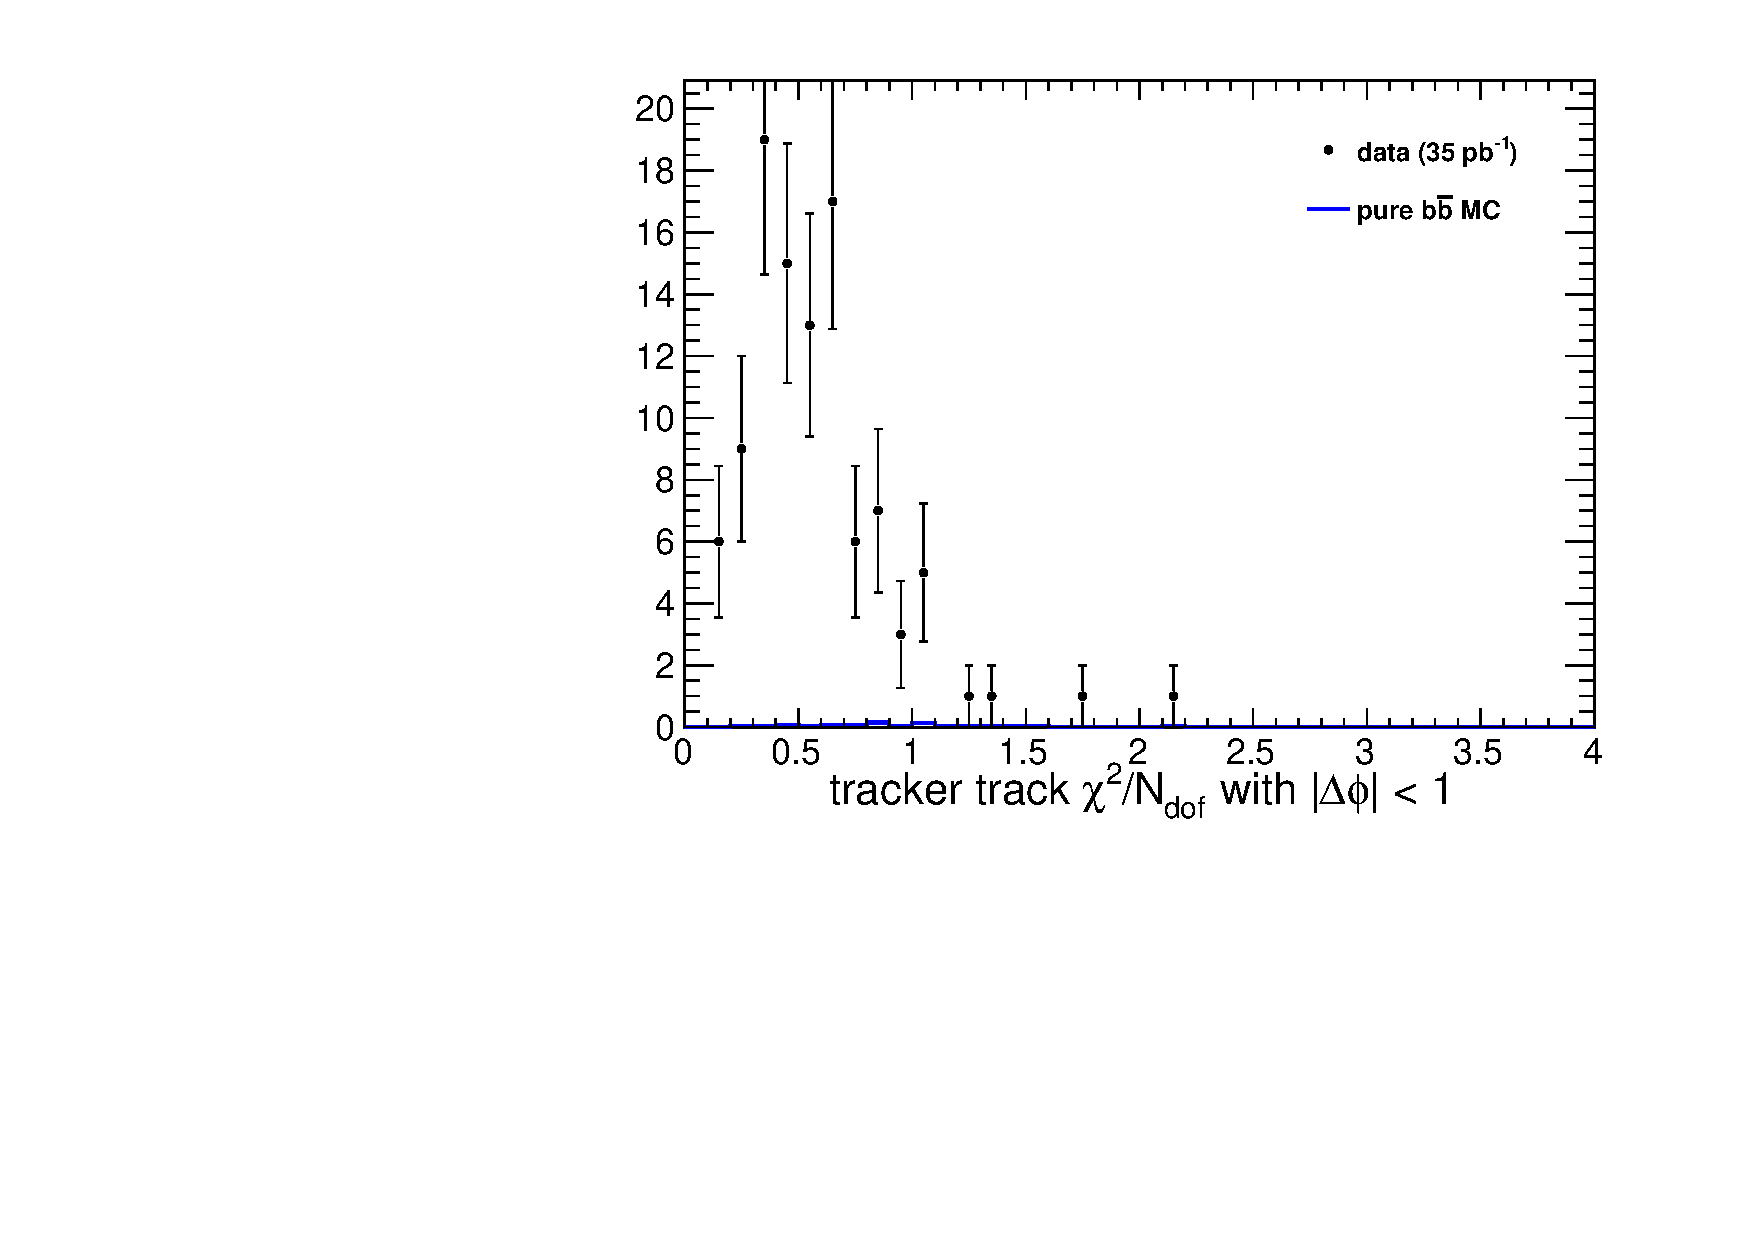
\includegraphics[width=0.43\linewidth]{dimuorphan_orphanchi2_collinear.pdf}

\scriptsize $\chi^2/N_\s{dof} \ll 1$ can happen in data if the APEs are too large (and would cause vertex probabilities to be biased toward 1, something else we've seen).  MC alignment is ideal.
\end{frame}

\begin{frame}
\frametitle{Diagnostic of $|\Delta\phi| < 1$ events}
\framesubtitle{$|\Delta\phi| < 1$ when the dimuon and the orphan are nearly collinear: \\ something that never happens in the $b\bar{b}$ MC}

Station 1 muon residuals ($x$) for the orphan

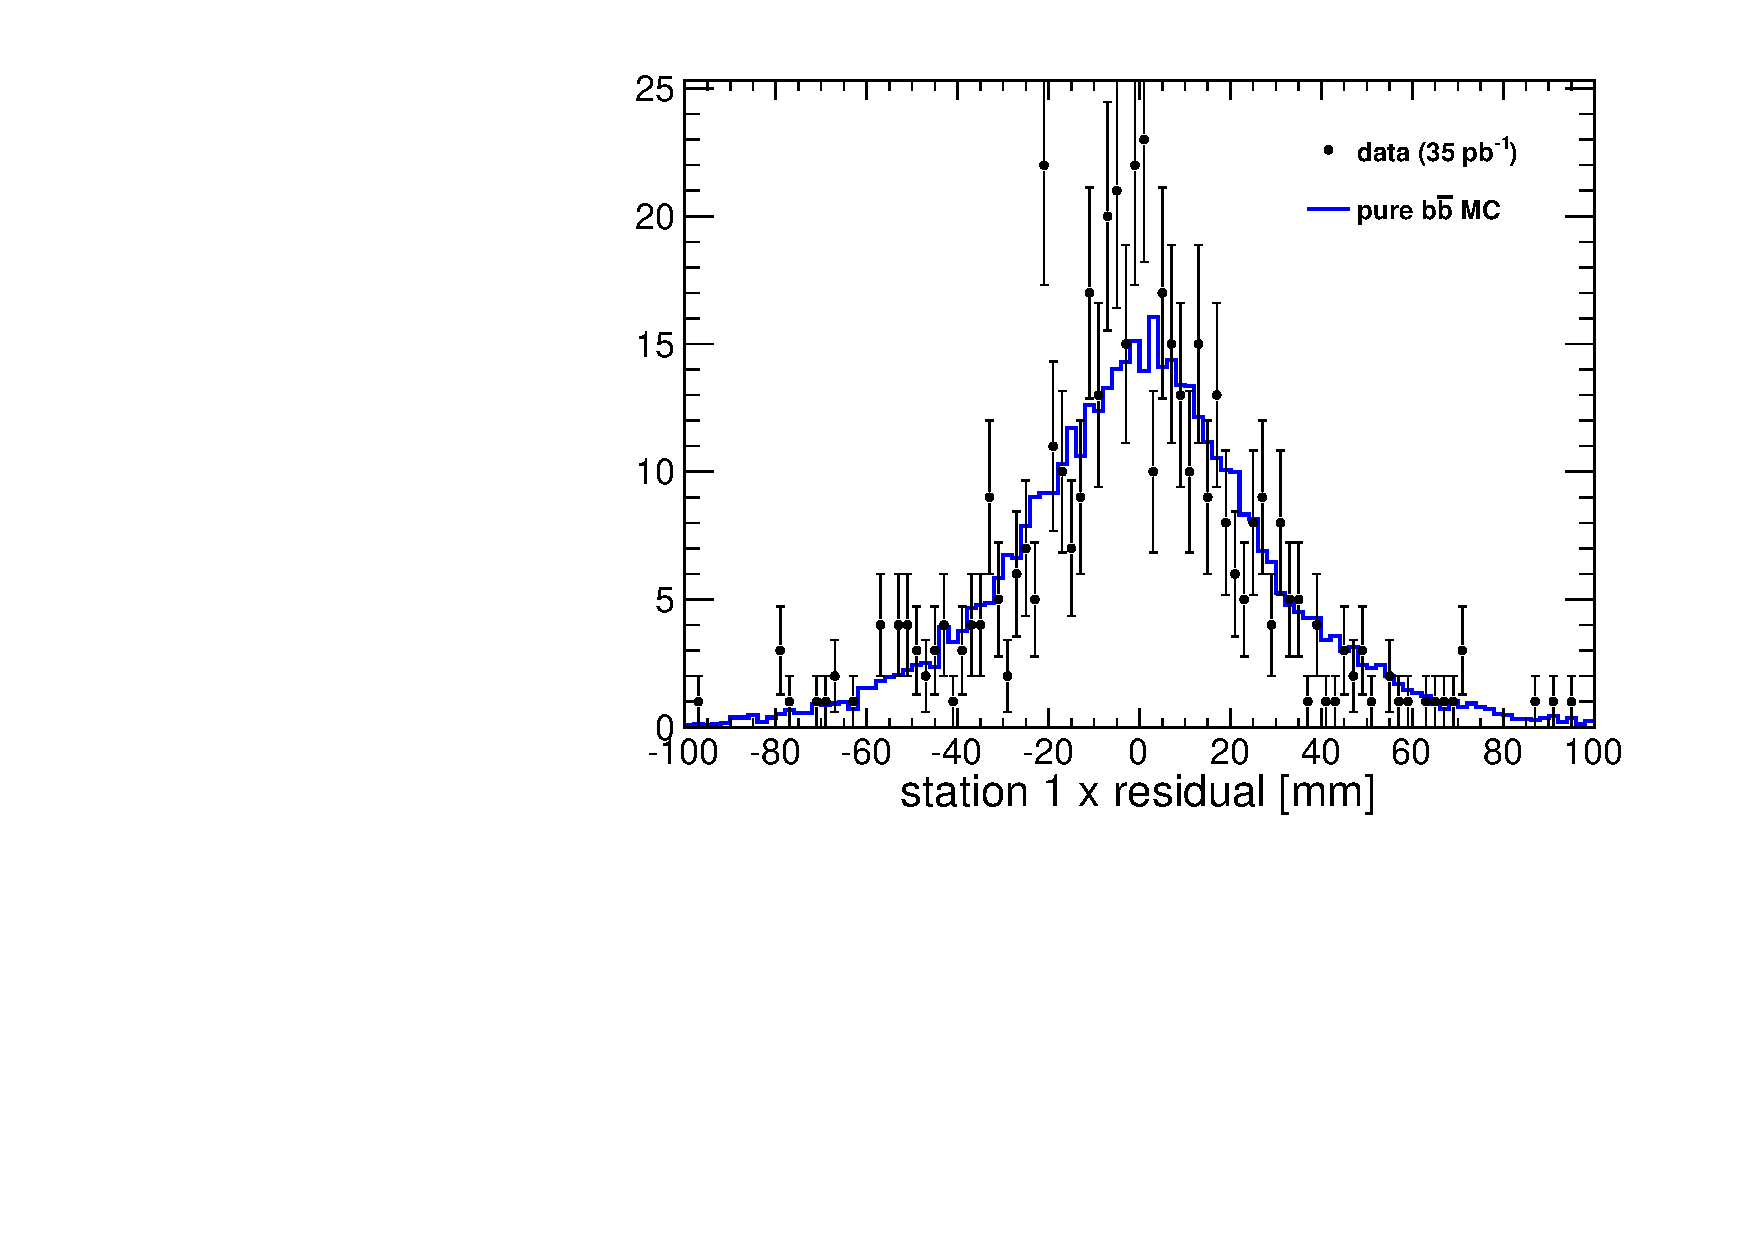
\includegraphics[width=0.45\linewidth]{dimuorphan_orphanst1x.pdf}
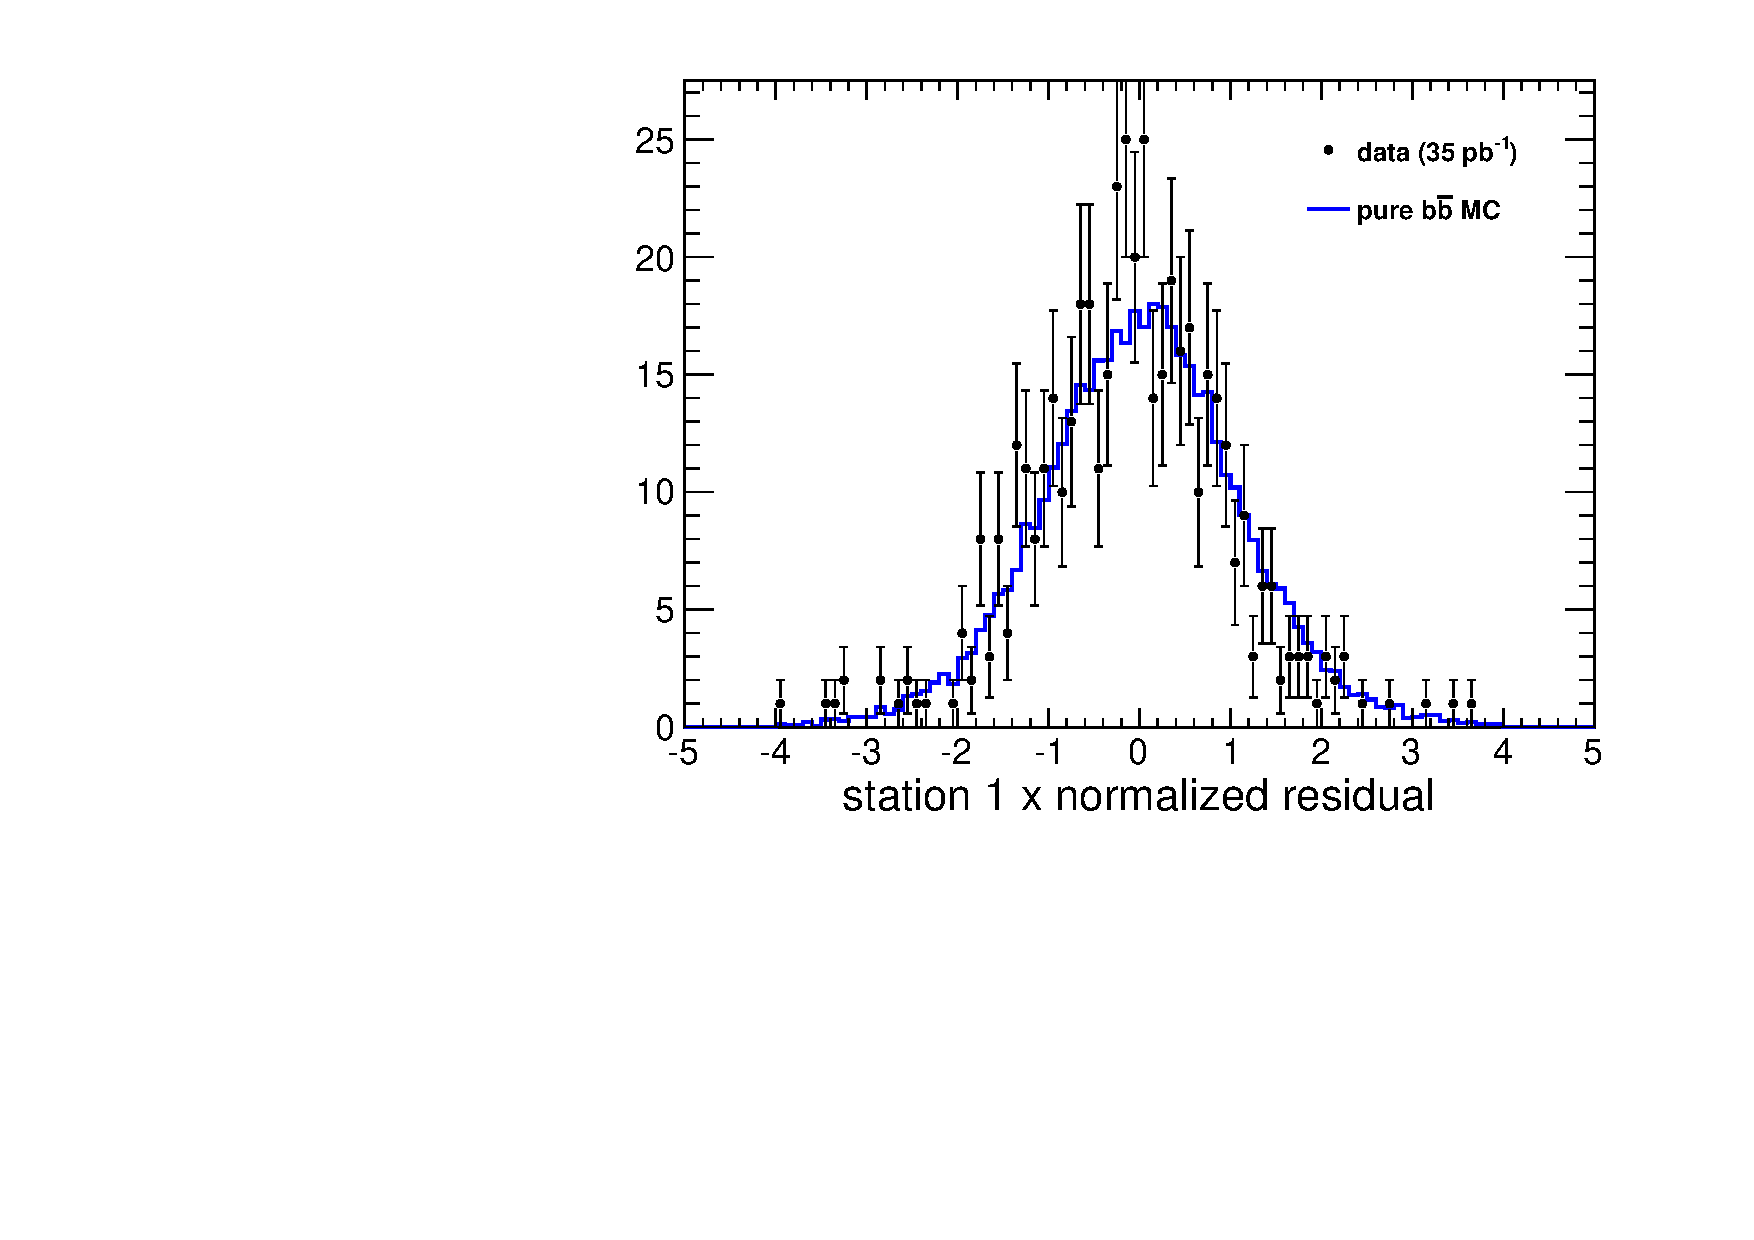
\includegraphics[width=0.45\linewidth]{dimuorphan_orphanst1xsig.pdf}

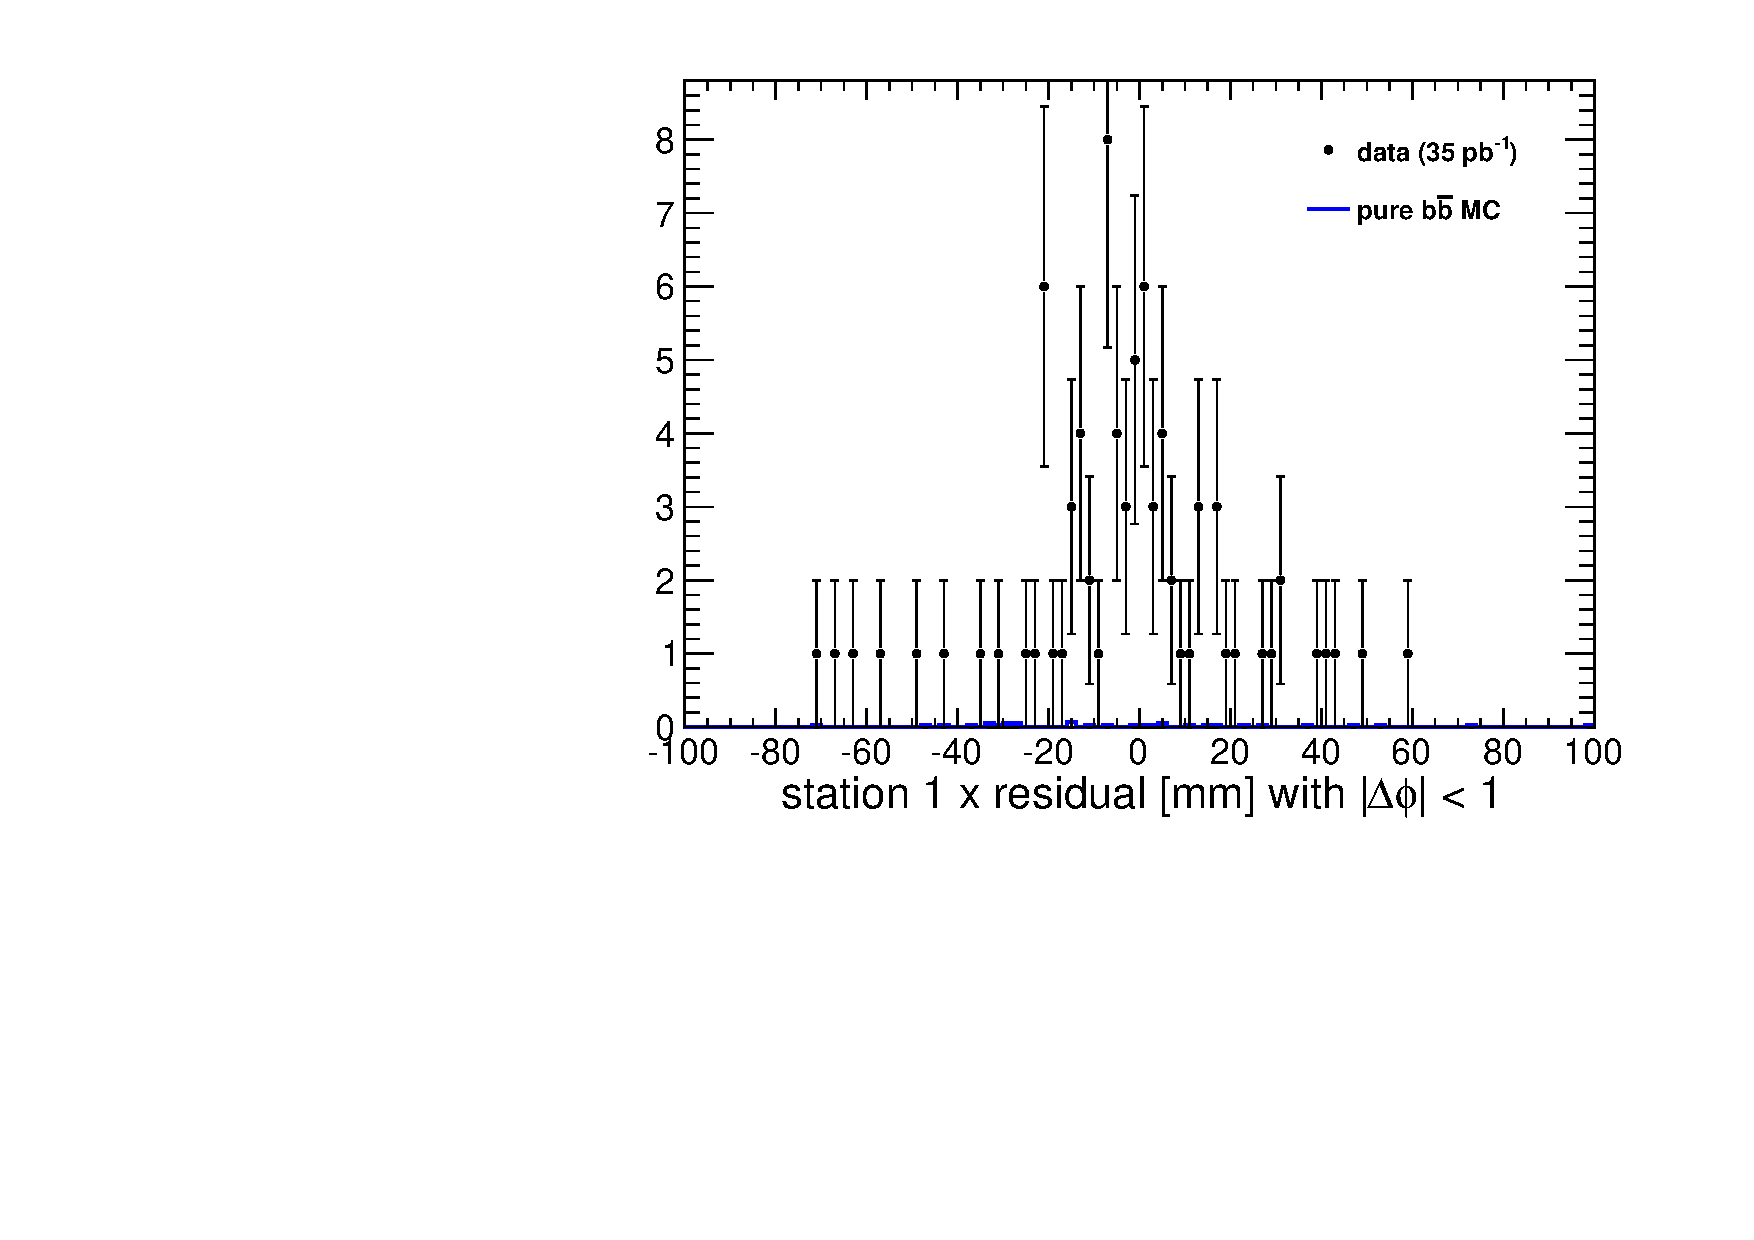
\includegraphics[width=0.45\linewidth]{dimuorphan_orphanst1x_collinear.pdf}
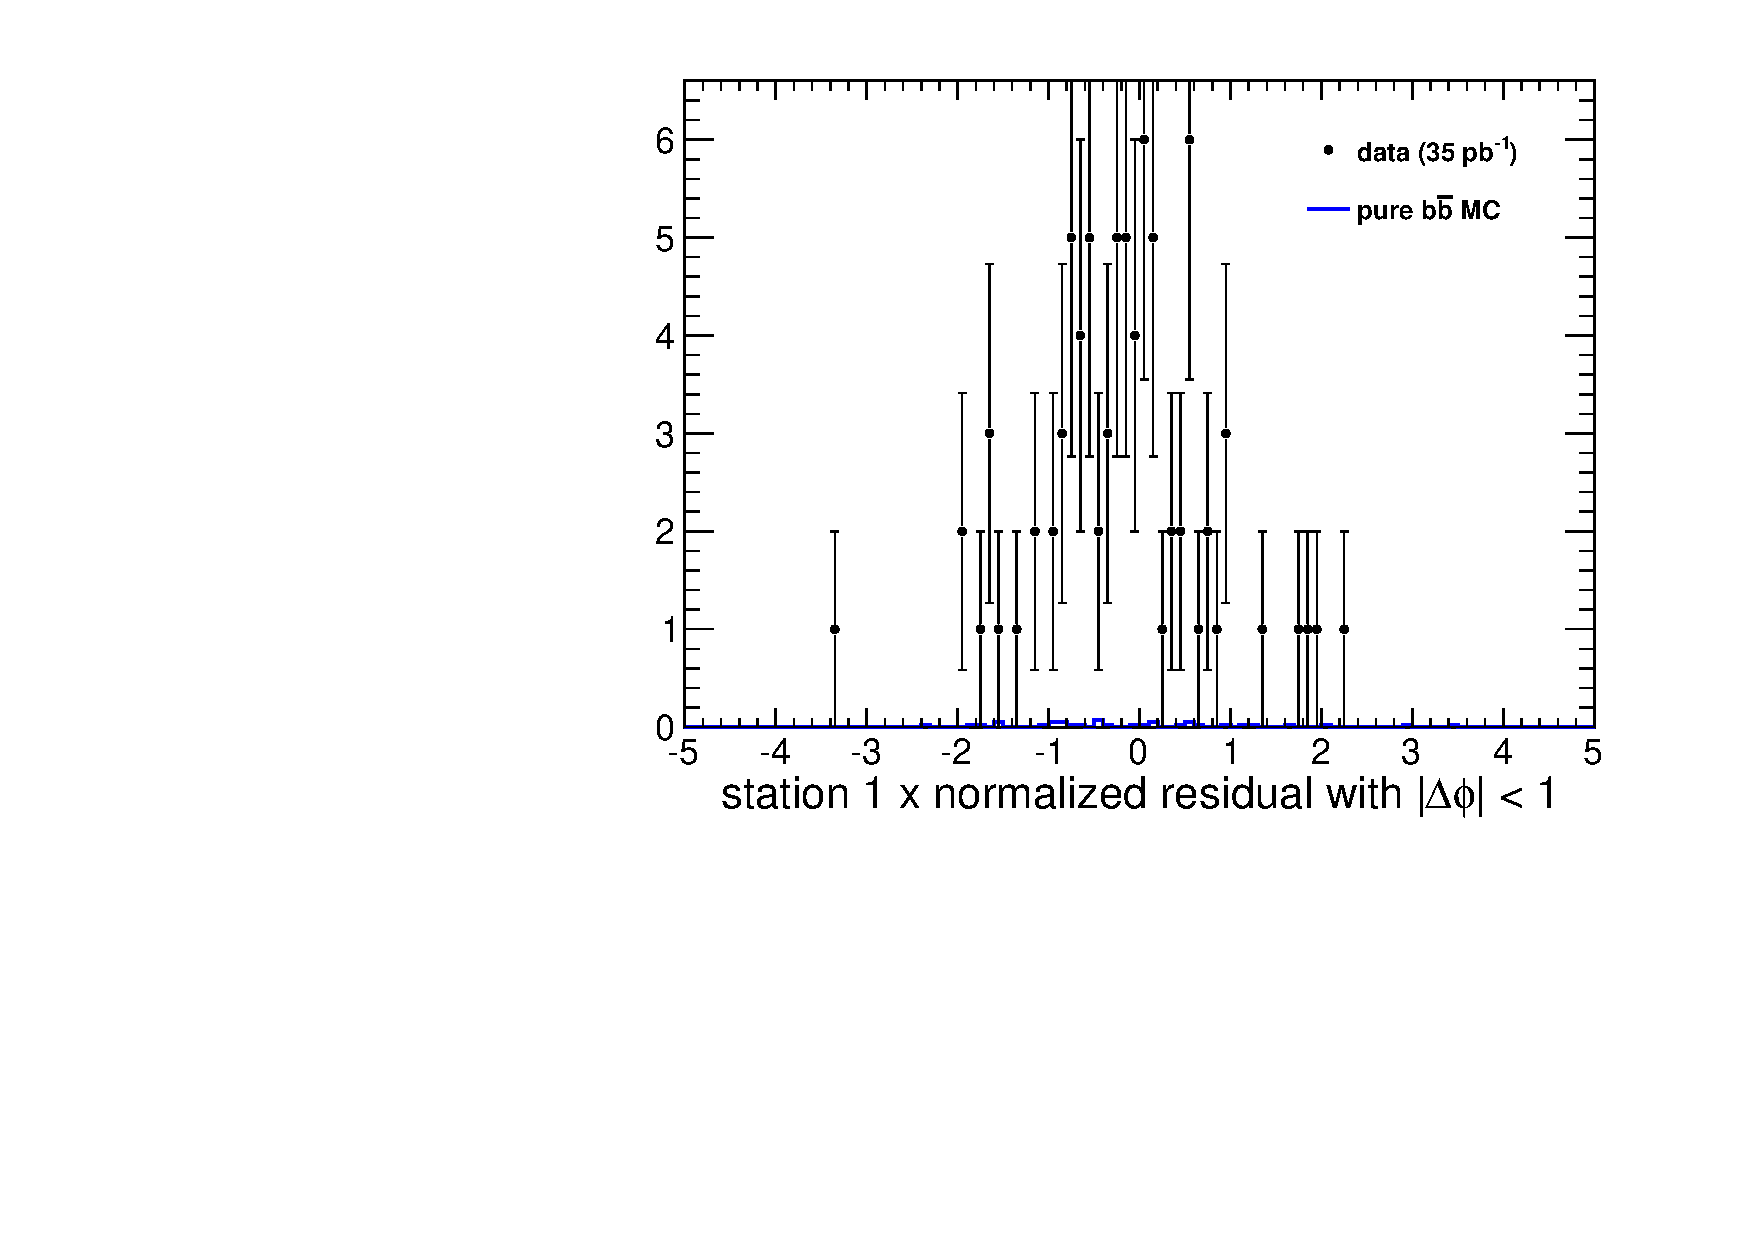
\includegraphics[width=0.45\linewidth]{dimuorphan_orphanst1xsig_collinear.pdf}
\end{frame}

\begin{frame}
\frametitle{Diagnostic of $|\Delta\phi| < 1$ events}
\framesubtitle{$|\Delta\phi| < 1$ when the dimuon and the orphan are nearly collinear: \\ something that never happens in the $b\bar{b}$ MC}

Station 1 muon residuals ($dx/dz$) for the orphan

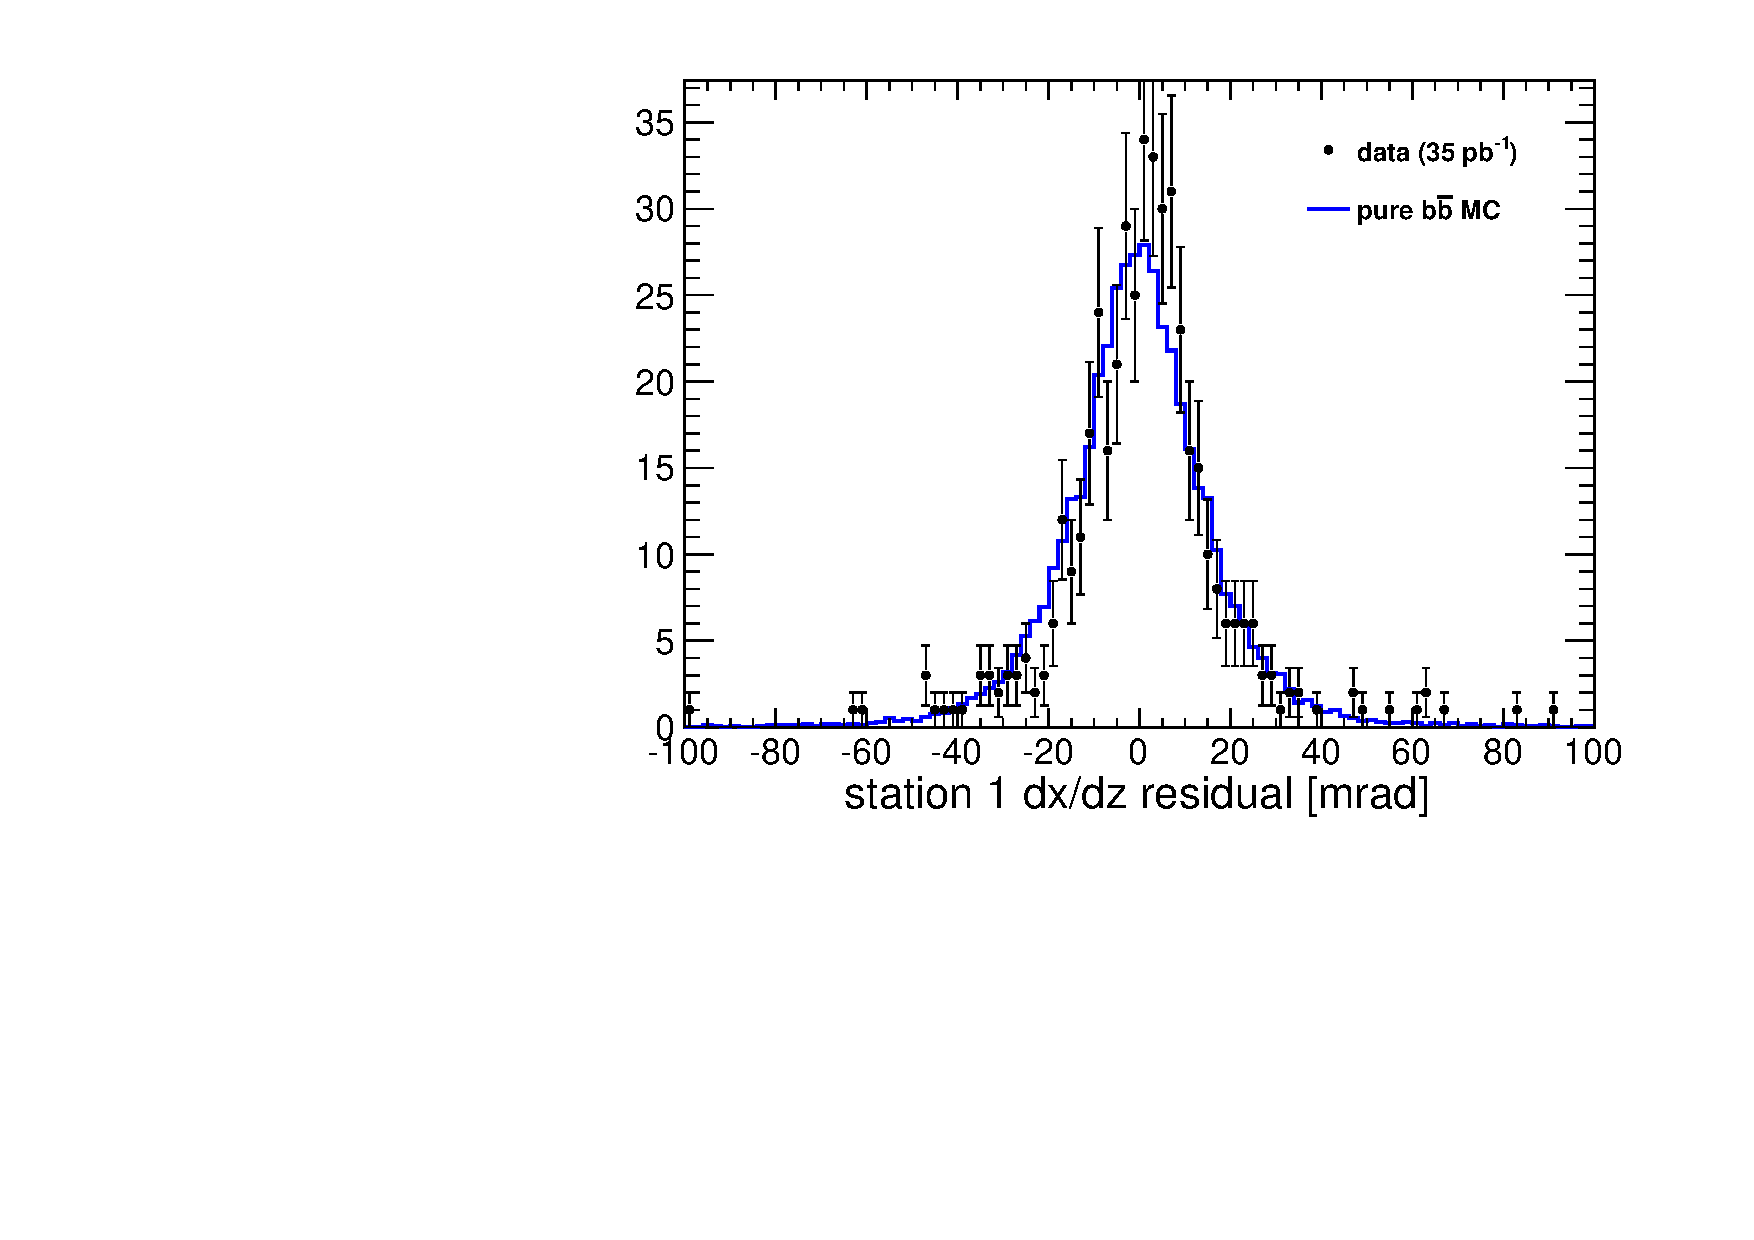
\includegraphics[width=0.45\linewidth]{dimuorphan_orphanst1dxdz.pdf}
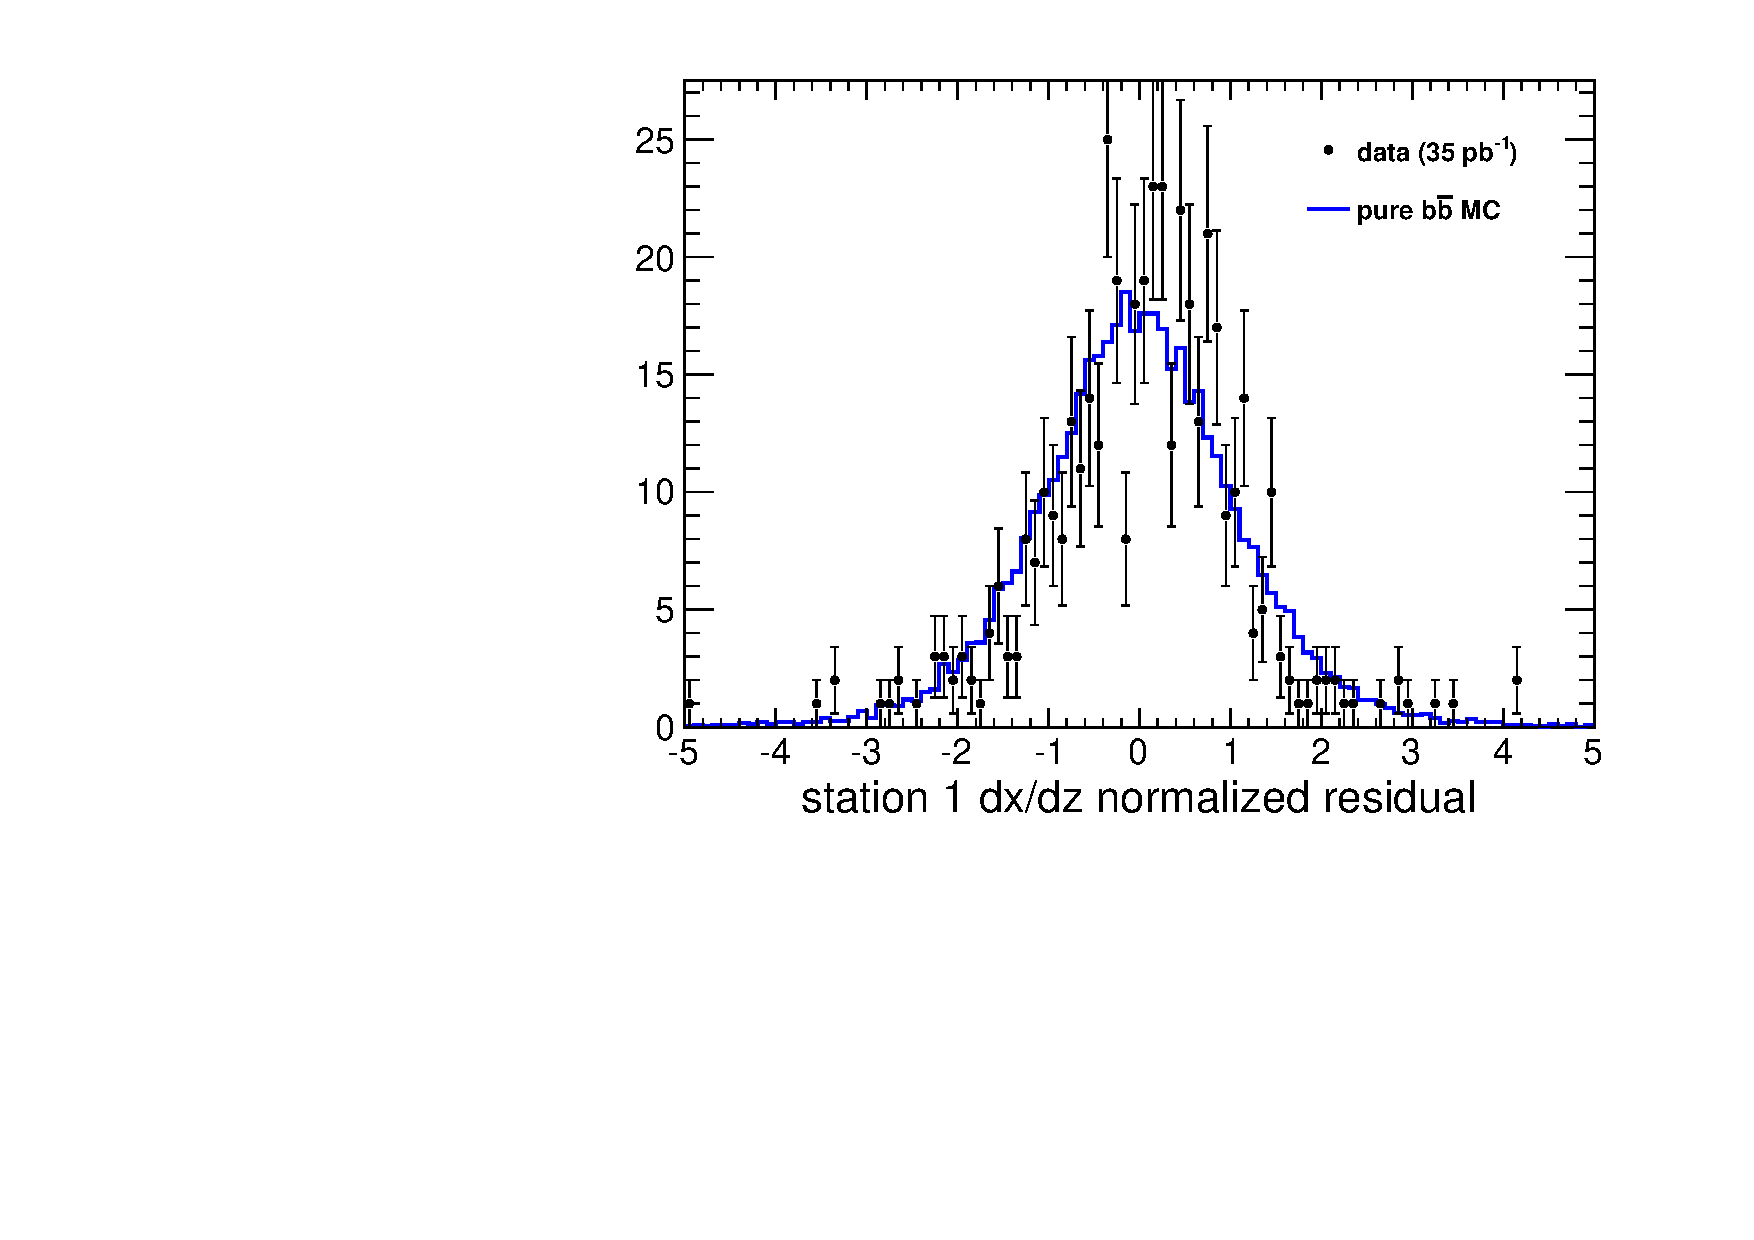
\includegraphics[width=0.45\linewidth]{dimuorphan_orphanst1dxdzsig.pdf}

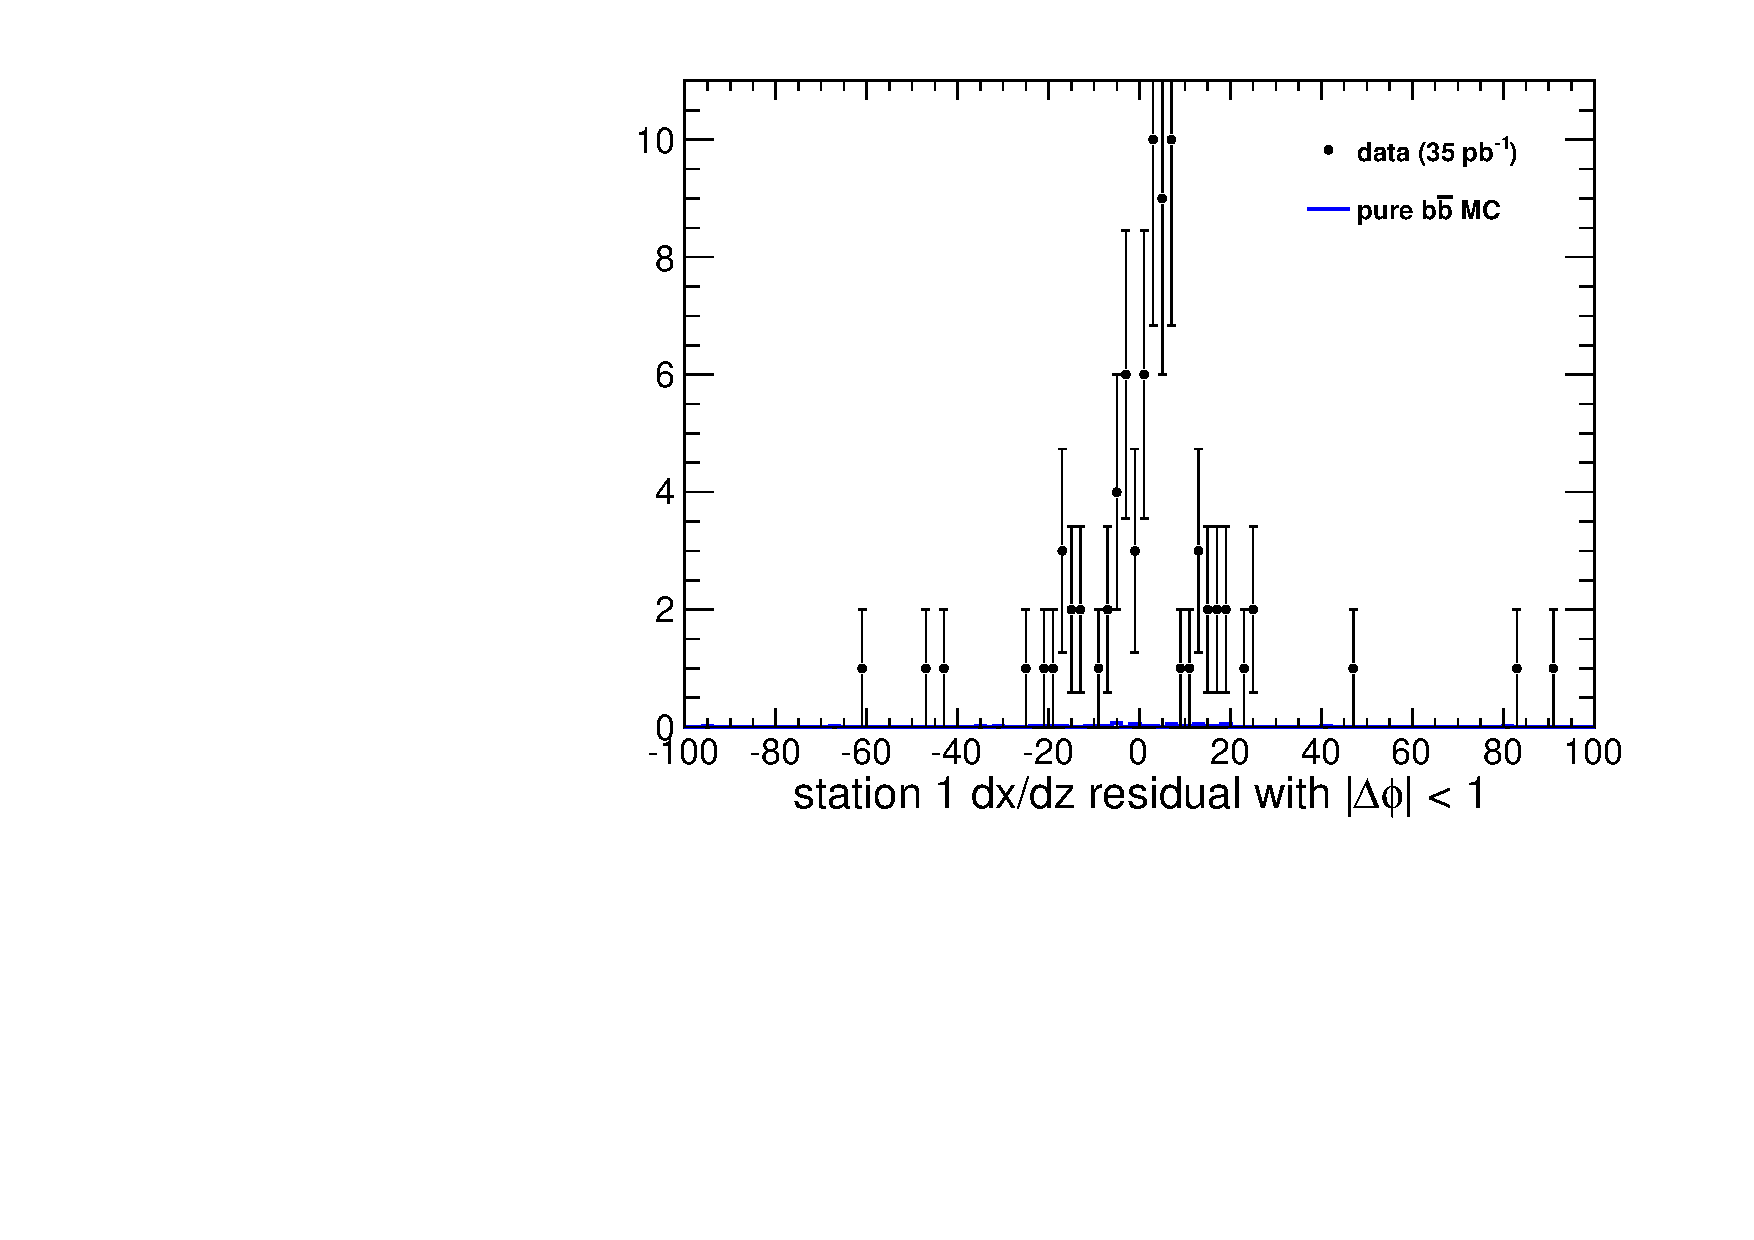
\includegraphics[width=0.45\linewidth]{dimuorphan_orphanst1dxdz_collinear.pdf}
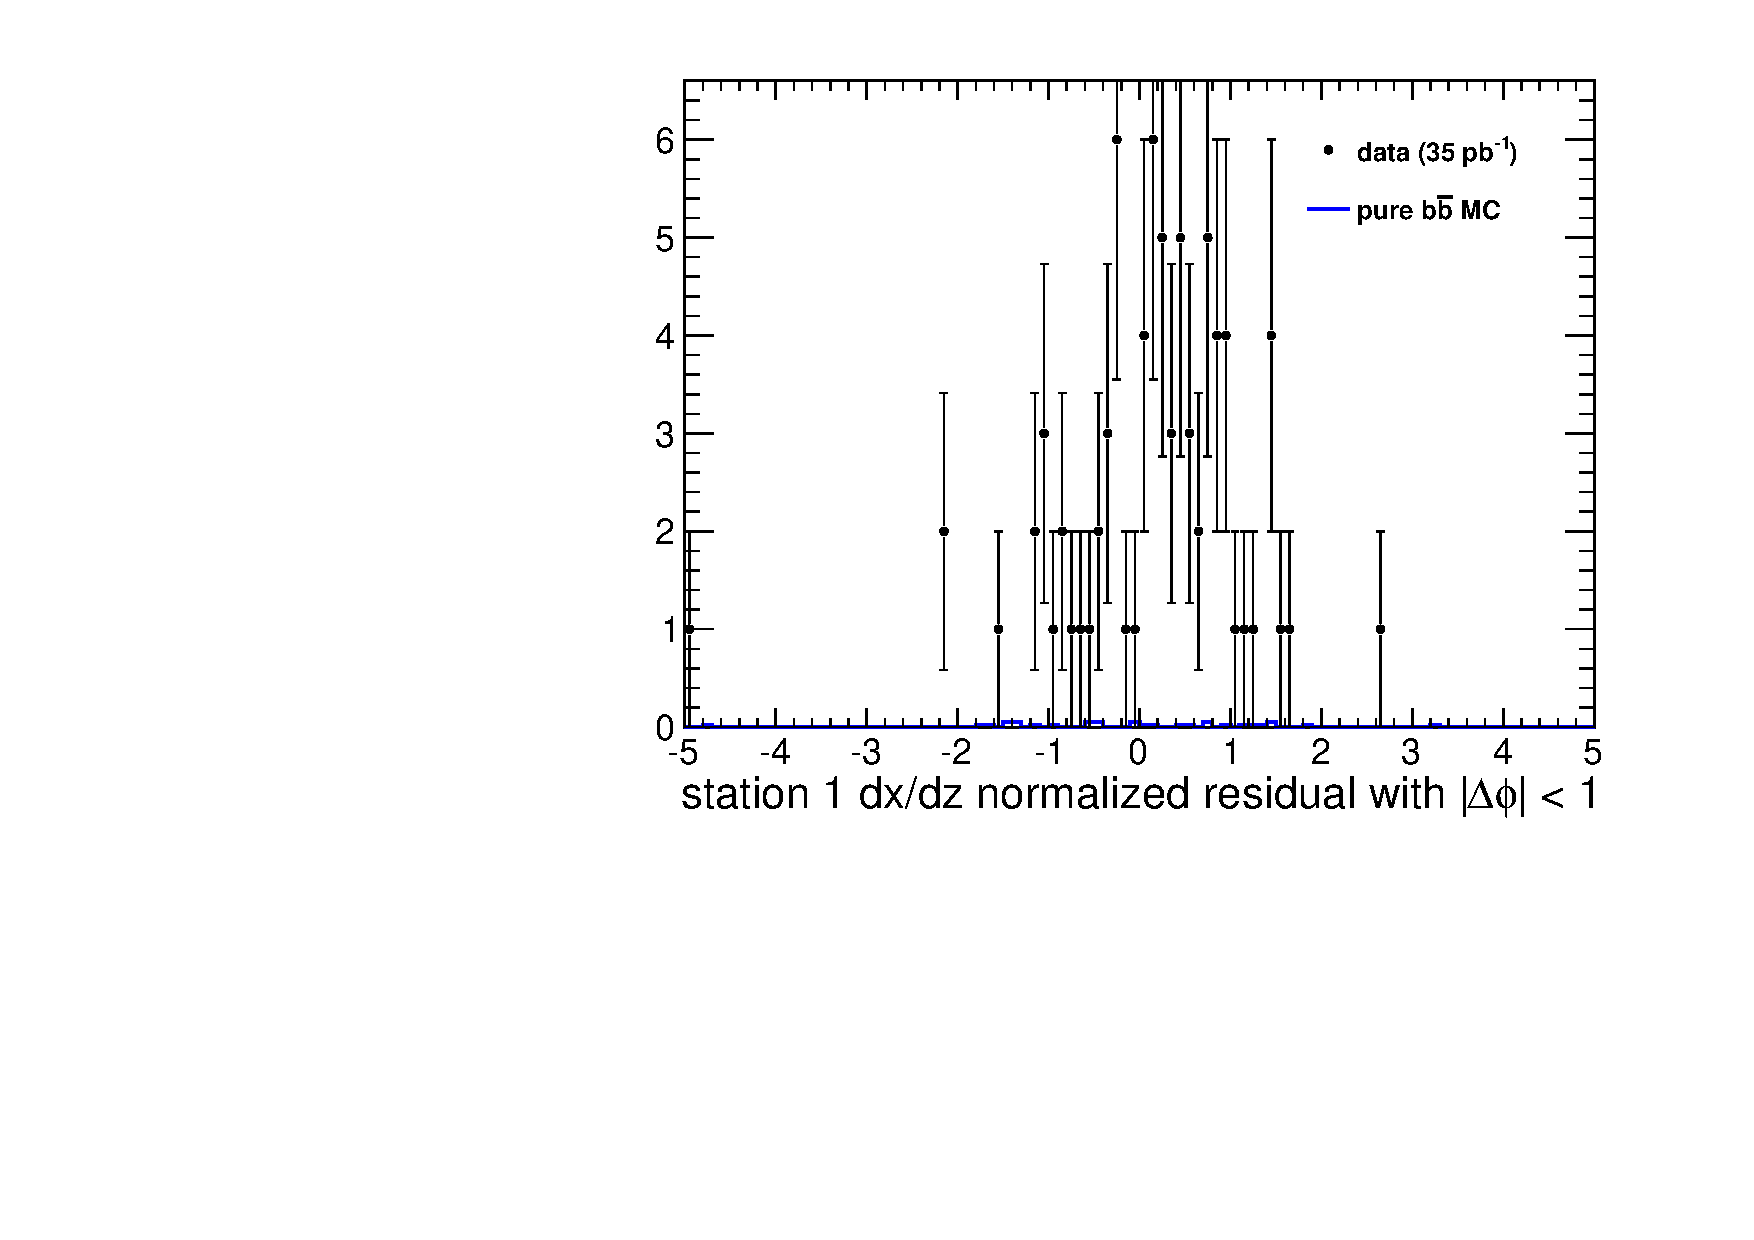
\includegraphics[width=0.45\linewidth]{dimuorphan_orphanst1dxdzsig_collinear.pdf}
\end{frame}

\begin{frame}
\frametitle{Conclusions}

\begin{itemize}
\item Now we have a complete set of background mass templates for the dimuon-dimuon signal region.
\begin{itemize}
\item the dimuon-dimuon signal region should have the ``central dimuon'' on the vertical axis (which contains the $p_T > 12$~GeV/$c^2$, $|\eta| < 1$ muon we used to satisfy the trigger) and the ``other dimuon'' on the horizontal axis
\item the background mass template for the ``central dimuon'' comes from the single-dimuon control sample (sent last time)
\item the background mass template for the ``other dimuon'' comes from this study with dimuon + orphan, allowing for unknown contributions from Standard Model resonances
\end{itemize}

\item The data and MC differ in how much boost the $b$-quarks get, but
\begin{itemize}
\item the orphan is always a good muon, even in these cases
\item the dimuon looks like a $b$-quark decay; it just looks like the whole event is boosted by other hadronic jets
\item invariant mass is insensitive to boosts
\end{itemize}

\item Moving on\ldots
\end{itemize}

\label{numpages}
\end{frame}

\end{document}
